\svnidlong
{$HeadURL$}
{$LastChangedDate$}
{$LastChangedRevision$}
{$LastChangedBy$}
\svnid{$Id$}


% preamble

In this Chapter we review 
models that yield $X$+\MET{} signatures,
where $X$ is a QCD parton or $\gamma, W, Z$ or $h$.

The primary simplified models for Dirac fermion DM studied and recommended by this Forum 
for early LHC Run-2 searches are detailed in this Chapter, 
comprising \spinzero and \spinone mediators. Section~\ref{sec:monojet_V} covers the
\schannel exchange of a vector mediator~\footnote{Colored vector mediators 
can be exchanged in the \tchannel, but there are no examples in literature so far.}, 
while we consider both \schannel and \tchannel exchange for scalar mediators in
Section~\ref{sec:monojet_scalar} and~\ref{sec:monojet_t_channel} respectively. 
\Spintwo mediators are briefly mentioned in Section~\ref{sec:spintwo}.
While these models are general and cover a broad set of signatures,
the discussion and studies are focused on the monojet final state. 
Details on final states with electroweak (EW) boson radiation and with heavy flavor quarks 
from diagrams arising within these models are also discussed in this Chapter.
%In the following paragraphs we present the peculiarities of these models that arise in the case of
%boson radiation, and present some examples of the relevant distributions for these final states.

A summary of the state of the art calculations and implementations for these models 
is provided in Table~%\ref{tab:summaryModels} % hardwire, because we don't use real caption on that table.
6.1. Section~\ref{app:MonojetLikeModels_Appendix}
details the implementation of these models that
have been used for the studies in this Chapter and that will be employed
for the simulation of early Run-2 benchmark models for LHC DM searches. 

%%%%%%%%%%%%%%%
%%%%%%%%%%%%%%%
%%%%%%%%%%%%%%%
% V/A SIMPLIFIED MODELS%
%%%%%%%%%%%%%%%
%%%%%%%%%%%%%%%
%%%%%%%%%%%%%%%

\section{Vector and axial vector mediator, \schannel exchange}
\label{sec:monojet_V}

A simple extension of the Standard Model (SM) is an
additional $U(1)$ gauge symmetry, where a Dark Matter
candidate particle has charges only under this new group.
Assuming that some SM particles are also charged under
this group, a new gauge boson can mediate interactions
between the SM and DM.   

%Lagrangian
We consider the case of a DM particle \chiDM of mass \mdm that is a Dirac fermion and where the production 
proceeds via the exchange of a \spinone mediator of mass \mMed in
the \schannel, illustrated in Fig.~\ref{fig:OP}.

\begin{figure}[h!]
\centering
  \unitlength=0.005\textwidth
  \vspace{0.5\baselineskip}
  \begin{feynmandiagram}[modelVmonojetParameters]
    \fmfleft{i1,i2}
    \fmfright{o1,o2}
    \fmftop{isr}
    \fmfbottom{pisr}
    % \fmf{dashes,tension=0.6,label={$\substack{{\Large V,,A}\\(m_{med},,\Gamma_{min,,med})}$}}{v1,v2}
    \fmf{wiggly,tension=0.6,label={\Large $V,,A(\mMed)$}}{v1,v2}
    \fmf{fermion}{o2,v2,o1}
    \fmf{fermion}{i2,visr,v1}
    \fmf{plain}{v1,pvisr,i1}
    \fmf{fermion,tension=0}{v1,i1}
    \fmfdot{v1,v2}
    \fmflabel{\Large ${g_q}$}{v1}
    \fmflabel{\Large ${g_{DM}}$}{v2}
    \fmflabel{\Large ${\bar{q}}$}{i1}
    \fmflabel{\Large ${q}$}{i2}
    \fmflabel{\Large ${\bar{\chiDM}(\mDM)}$}{o1}
    \fmflabel{\Large ${\chiDM(\mDM)}$}{o2}
    \fmf{gluon,tension=0}{visr,isr}
    \fmf{phantom,tension=0}{pvisr,pisr}
    \fmflabel{\Large ${g}$}{isr}
  \end{feynmandiagram}
%\caption[][\baselineskip]{Representative Feynman
\caption{Representative Feynman
diagram showing the pair production of Dark Matter particles in association with a parton from the initial state via a vector or axial-vector mediator.
The cross section and kinematics depend upon
the mediator and Dark Matter masses, and the mediator couplings to Dark Matter and quarks respectively: ($\mMed ,\, \mDM ,\, \gDM ,\, \gq)$. }
\label{fig:OP}
\setfloatalignment{t}
  \vspace{0.5\baselineskip}
\end{figure}

We consider two models with vector and axial-vector couplings
between the \spinone mediator $\Zprime$ and SM and DM fields, with
the corresponding interaction Lagrangians:

\begin{align}
\label{eq:AV} 
\mathcal{L}_{\mathrm{vector}} &= \gq \sum_{q={u,d,s,c,b,t}}  \Zprime_{\mu} \bar{q}\gamma^{\mu}q + \gDM \Zprime_{\mu} \bar{\chiDM}\gamma^{\mu}\chiDM \\
\mathcal{L}_{\rm{axial-vector}} &= \gq \sum_{q={u,d,s,c,b,t}}  \Zprime_{\mu} \bar{q}\gamma^{\mu}\gamma^5q + \gDM \Zprime_{\mu} \bar{\chiDM}\gamma^{\mu}\gamma^5\chiDM.
\end{align}
The coupling \gq is assumed to be universal to all quarks.
It is also possible to consider other models in which mixed vector and axial-vector couplings are considered, 
for instance the couplings to the quarks are axial-vector whereas those to DM are vector. 
%We recommend the models with
%pure vector couplings or pure axial-vector couplings.
%\Todo{Studies have been performed to see if the case of a mixed coupling can be simply extracted from the other models by some reweighting procedure to take account of the difference in cross section. This would assume that the difference between the pure and mixed couplings case does not affect the kinematics of the event. Note, though, that in the mediator rest frame, the angular distribution of the DM relative to the mediator direction of motion has the form: $1+z^2+2*C*z$ ($z=\cos\theta$), with the second term only present in the mixed case. This may lead to acceptance differences.}
%Definition of minimal width
As mentioned in the Introduction, when no additional visible or invisible decays contribute to the width of the mediator, 
the minimal width is fixed by the choices of couplings \gq and \gDM. The effect of larger 
widths is discussed in Section~\ref{paragraph:nonminimalwidth}. 
For the vector and axial-vector models, the minimal width is:

\begin{align}
\label{eq:monojet_min}
\Gamma^{\textrm{V}}_\textrm{min} &= 
\frac{\gDM^2 \mMed}{12\pi}\left(1+\frac{2 \mDM^2}{\mMed^2} \right)\beta_{DM} \theta(\mMed-2\mDM)\\\nonumber
 &+ \sum_q \frac{3 \gq^2 \mMed}{12\pi}\left(1+\frac{2 m_q^2}{\mMed^2} \right)\beta_q \theta(\mMed-2m_q),\\
\Gamma_{\textrm{min}}^{\rm{A}}&=\frac{\gDM^2 \mMed}{12\pi} \beta_{DM}^{3} \theta(\mMed-2\mDM)\\\nonumber
   &+ \sum_q \frac{3 \gq^2 \mMed}{12\pi}\beta_q^{3} \theta(\mMed-2m_q)\;.
\end{align}
$\theta(x)$ denotes the Heaviside step function, and
$\beta_f=\sqrt{1-\frac{4 m_f^2}{\mMed^2}}$ is the velocity of the
fermion $f$ with mass $m_f$  in the mediator rest frame.
Note the color factor 3 in the quark terms.
Figure\,\ref{fig:monojet_width_V} shows the minimal width as a function of mediator mass for both vector and axial-vector mediators assuming
$\gq=\gDM=1$. With this choice of the couplings, the dominant contribution to the minimal width comes from the quarks, due 
to the combined quark number and color factor enhancement. %CD: before was:"and the large number of them."
We specifically assume that the vector mediator does not couple to leptons.  If such a coupling were present, it would have a minor effect in increasing the mediator width, but it would also bring in constraints from measurements of the Drell-Yan process that would unnecessarily restrict the model space.

\begin{figure}
\centering
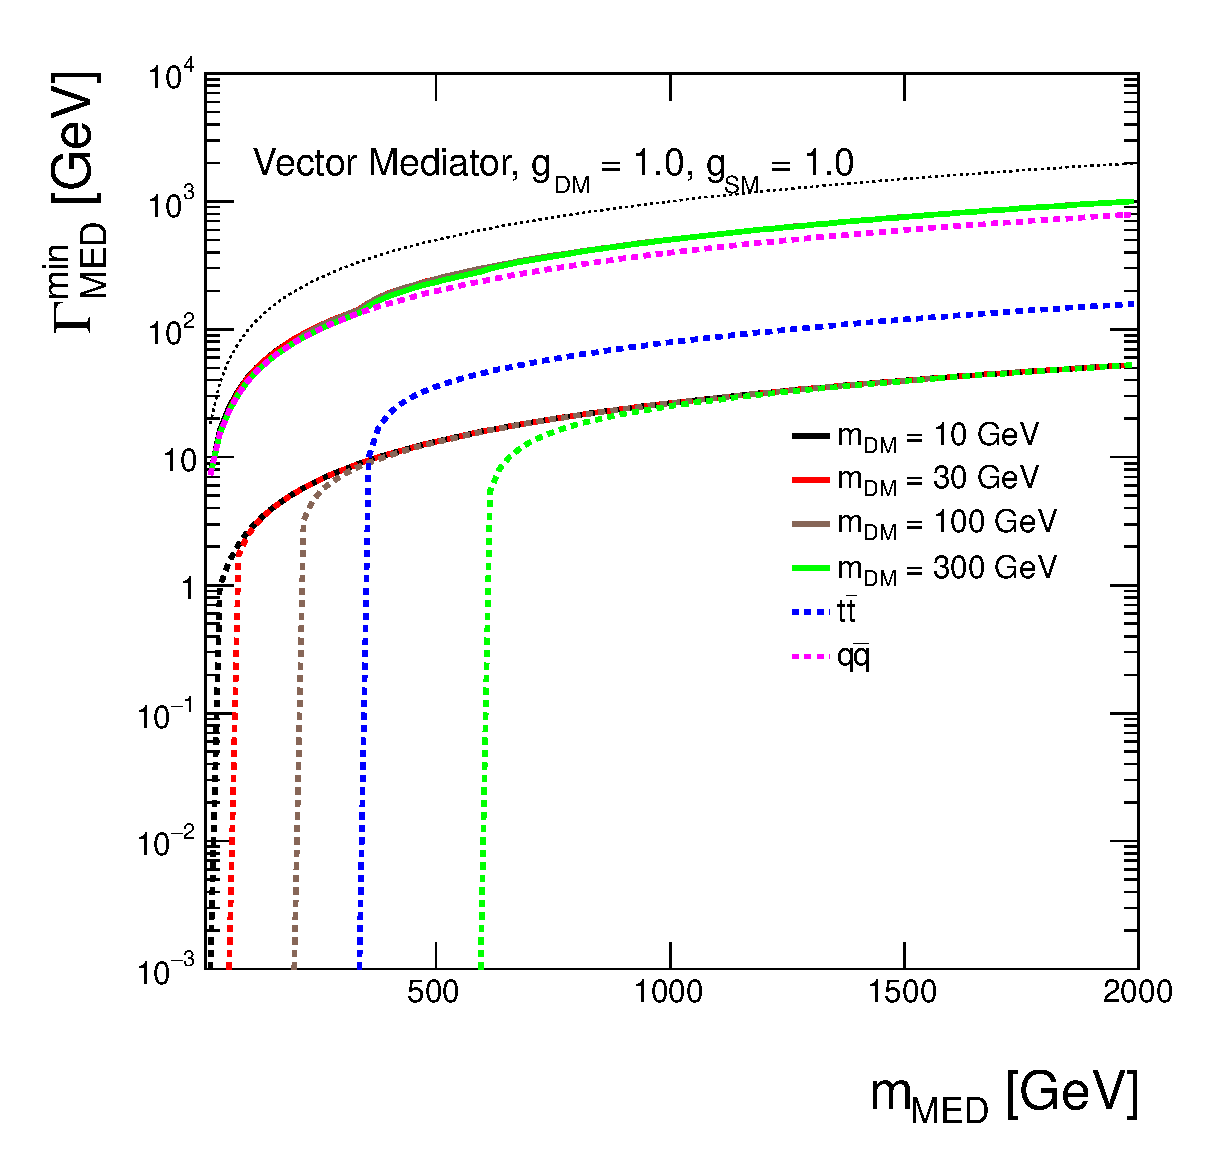
\includegraphics[width=0.95\textwidth]{figures/monojet/width_V.eps}
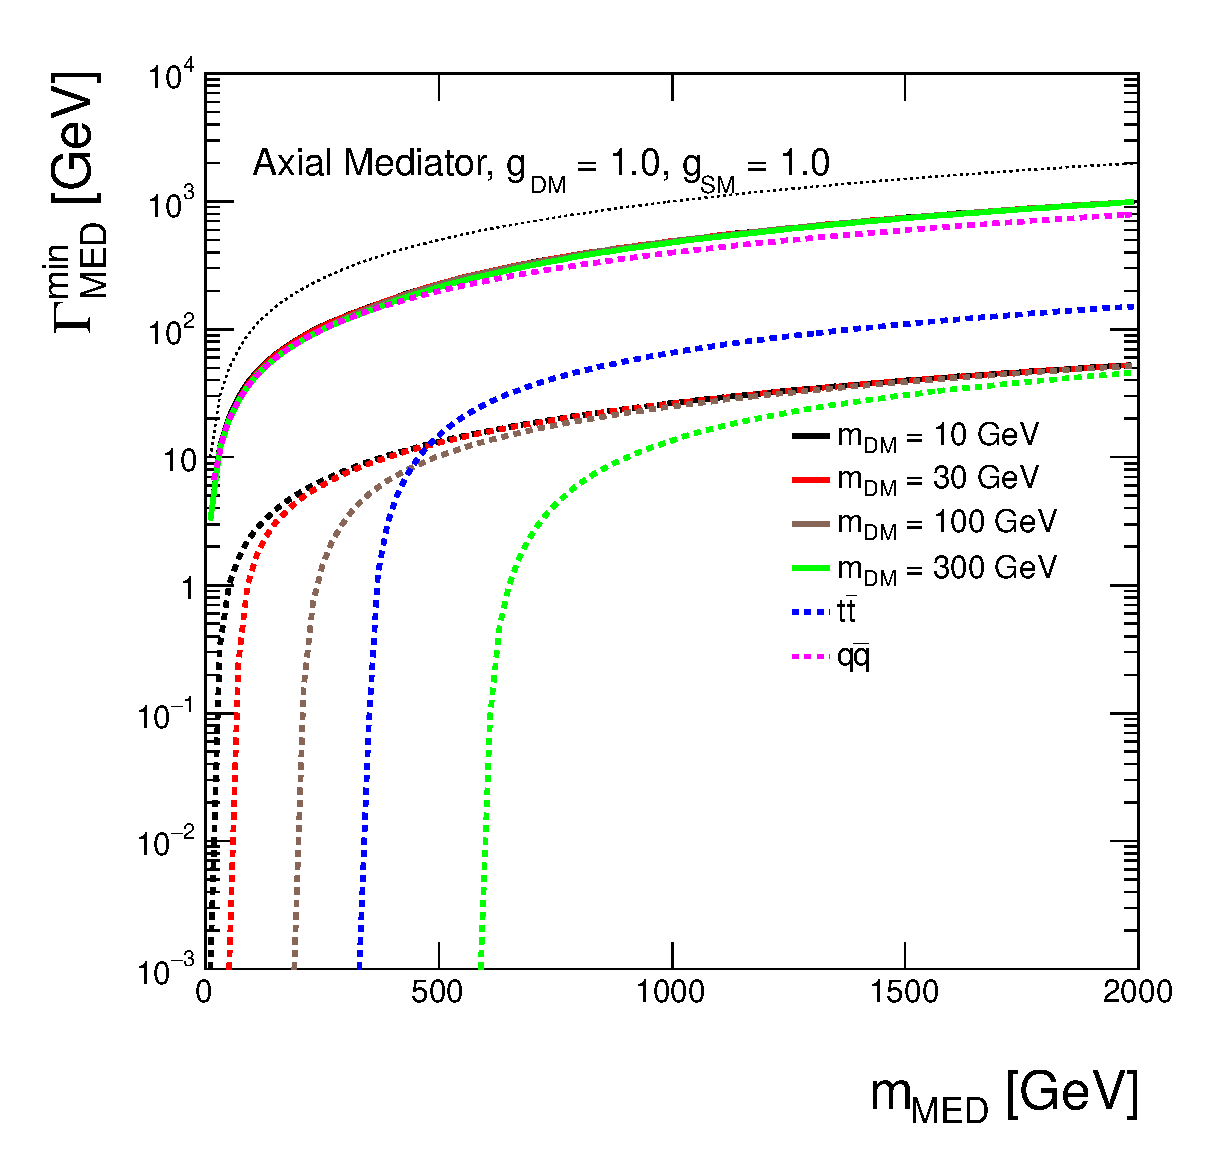
\includegraphics[width=0.95\textwidth]{figures/monojet/width_A.eps}
\caption{Minimal width as a function of mediator mass for vector and axial-vector mediator assuming couplings of 1. The total width is shown as solid lines for Dark Matter masses of 10~\gev, 30~\gev, 100~\gev and 300~\gev in black, red, brown and green, respectively. The individual contributions from Dark Matter are indicated by dotted lines with the same colors. The contribution from all quarks but top is shown as magenta dotted line and the contribution from top quarks only is illustrated by the dotted blue line. The dotted black line shows the extreme case $\Gamma_{\rm{min}}=\mMed$.}
\label{fig:monojet_width_V}
\end{figure}

Therefore, the minimal set of parameters under consideration for these two models is
\bea
\left\{~\gq, ~ \gDM, ~\mDM,~\mMed,\right\} \,.
\eea
together with the spin structure of their couplings. 

A thorough discussion of these models and their parameters can also be found in~\cite{Buchmueller:2014yoa}.
 
%The two simplified models described here have four free parameters: mediator mass $\mMed$, Dark Matter mass $\mDM$, coupling of the mediator to quarks $\gq$ and coupling of the mediator to Dark Matter $\gDM$,

These simplified models are known and available in event generators at NLO + PS accuracy, as detailed in Section~\ref{sec:monojet_implementation}. 
Results in this Section have been obtained using the model implementation within the \powheg generator (\textsc{v3359}) \cite{Haisch:2013ata}.

In addition, for the vector models considered, initial and final state radiation of a $Z'$ can occur which can appear as a narrow jet if it decays hadronically and may not be distinguishable from a QCD jet, thus accounting for some fraction of the monojet signal. The ISR and FSR of $Z'$ becomes more important at large values of the couplings~\cite{Bai:2015nfa}. 

\subsection{Parameter scan}
\label{sub:parameter_scan_monojet}

In order to determine an optimal choice of the parameter grid for the simulation of early Run-2 benchmark models, dependencies of the kinematic quantities and cross sections on the model parameters have been studied. Only points that are kinematically distinct will be fully simulated, while instructions on how to rescale the results according to models with different cross sections are presented in Section~\ref{sec:monojet_scaling}. The following paragraphs list the main observations from the scans over the parameters that support the final proposal for the benchmark signal grid.

\subsubsection{Scan over the couplings}

To study the dependence of kinematic distributions on the coupling strength, samples were generated where a pair of $\mDM=10$~\gev Dark Matter particles is produced on-shell from the mediator of $\mMed=1$~\tev. 
Figure~\ref{fig:monojet_scan_V_g} compares the shapes of the \MET distribution for the different choices of the coupling strength. This is a generator-level prediction with no kinematic selections or detector simulation. Coupling values in the scan range 0.1--1.45, fixing $\gq=\gDM$, correspond to a rough estimate of the lower sensitivity of mono-jet analyses and a maximum coupling value such that $\Gamma_{\rm{min}} < \mMed$. We observe that the shapes of the \MET or jet \pT distributions do not depend on the couplings (and consequently the width) in the ranges considered. A large width of the mediator implies a broad integral over the contributing parton distributions, which might not be well approximated by the midpoint of this integral.  This study shows that the effect, in the \pT distribution of the observed gluon, is not important.

Based on similar findings for different choices of
\mMed and \mDM, we conclude that the shapes of
kinematic distributions are not altered
by coupling variations, neither for the on-shell Dark Matter production where $\mMed>2\mDM$,
nor for the off-shell DM production where $\mMed<2\mDM$. Only the production cross sections change.
Differences in kinematic distributions are expected only close to the transition region where both on-shell and off-shell decays occur.

\begin{figure*}
\centering
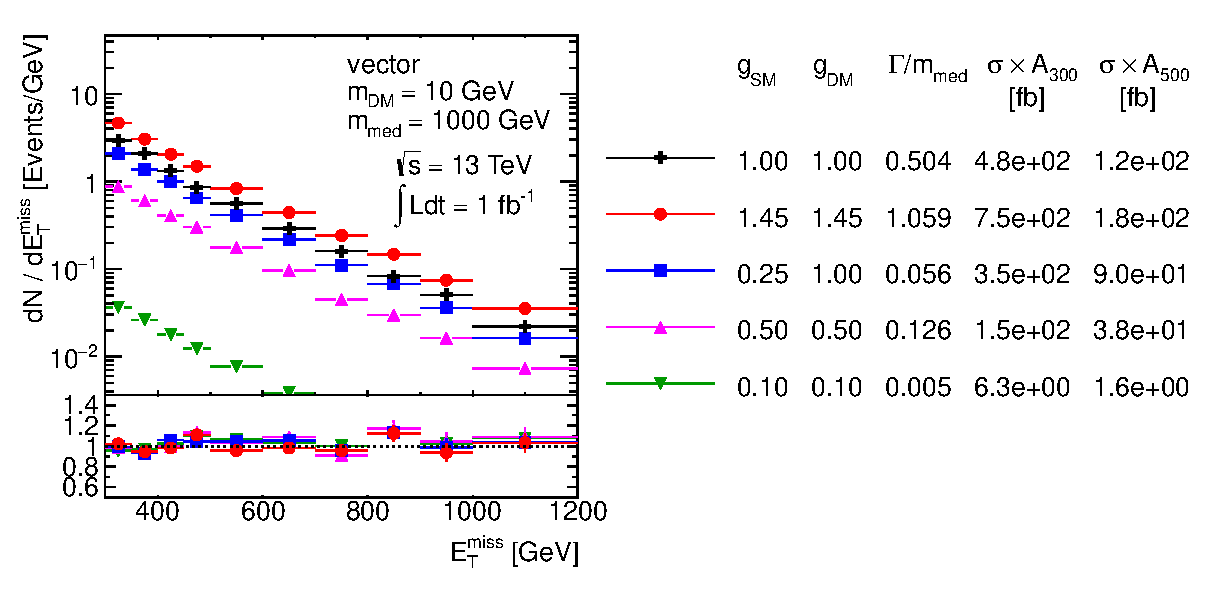
\includegraphics[width=0.95\textwidth]{figures/monojet/scan_g_V_10_1000.eps}
\caption[][-28pt]{Scan over couplings. The $\MET$ distribution is compared for the vector mediator models using the parameters as indicated. Ratios of the normalized distributions with respect to the first one are shown. $A_{300}$ and $A_{500}$ in the table denote the acceptance of the $\MET>300$~\gev and $\MET>500$~\gev cut, respectively.}
\label{fig:monojet_scan_V_g}
\end{figure*}

%When small coupling strengths are combined with extremely heavy mediators, one must take particular care to integrate over all values of the Dark Matter pair invariant mass, down to the lowest values for which the \MET satisfies threshold requirements. See the Appendix \ref{sec:monojet_implementation} page \pageref{thought:heavynarrowmediators} for details.

Special care needs to be taken when coupling strengths are combined with extremely heavy mediators.
Figure\,\ref{fig:monojet_narrow} suggests a change in the shape of the
\MET distribution for a $\mMed=5$~\tev mediator
once $\Gamma_{\rm{min}}/\mMed$ is of the order of a percent or lower.
Such heavy mediators, although inacessible by the LHC data, are interesting since they provide a good approximation for benchmark EFT models.
The observed difference among the simplified models in the plot arises from the fact that the region of low invariant masses of the Dark Matter pair, $m_{\bar{\chiDM}\chiDM}$, is suppressed due to narrow Breit-Wigner peak that only probes a narrow window of parton distribution functions. For wider mediators, the low mass region is significantly enhanced by parton distribution functions at low Bjorken $x$, as illustrated in Fig.\,\ref{fig:monojet_mchichi}(a).
This explains why the sample with the narrowest mediator in Fig.\,\ref{fig:monojet_narrow} is heavily suppressed in terms of production cross section and also gives different \MET shape.
%In general, for such extreme parameter choices the EFT model should give the correct answer.
Furthermore, Fig.\,\ref{fig:monojet_narrow} compares the vector model with 5~\tev mediator to the D5 EFT sample and reveals that the simplified models with larger mediator widths (e.g. for couplings of 1 where $\Gamma_{\rm{min}}/\mMed\sim0.5$) are the ones resembling the kinematics of contact interactions. This is because the production in the EFT model is always off-shell, i.e. no peak in the $m_{\bar{\chiDM}\chiDM}$ distribution is present.
In case of narrow width mediators, e.g. $\Gamma_{\rm{min}}/\mMed\sim0.05$, even larger mediator masses need to be chosen in order to significantly suppress the peak in the $m_{\bar{\chiDM}\chiDM}$ distribution and reproduce the kinematic shapes of an EFT model. Figure\,\ref{fig:monojet_mchichi}(b) verifies that the choice of 10~\tev mediator mass is sufficient to achieve that.


%\Todo{Refer to results of ongoing study in Section 6.}
%CD: commented out, we have to ask for having 7 TeV mediators
% In case the simplified model calculation does not reproduce the EFT result, the phase space generation of the simplified model has to be carefully examined in order to understand the cause of the problem. Fortunately, this is a rather academic discussion as such extreme corners of the parameter space are not going to be considered for presentation of Run-2 results.

%Uli: as fabio says, increasing bwcutoff might improve things in the case you are considering
%
%for a mediator with mass M = 7~\tev and width Gamma = 36~\gev, i think the correct way to do this calculation is to work in an EFT; this should give you the correct result
%
%in fact, if your simplified model calculation does not reproduce the EFT result for such extreme parameter choices, you have to carefully look at the phase-space generation of the simplified model calculation (as you did). at the end you probably have to tailor the phase-space generator of \madgraph, \powheg, etc. to get it right; this will be non-trivial since phase-space generation is an art! furthermore, one has to do this process 
%by process and the difficulties will increase from mono-jet to ttbar + \MET, etc. 

%\begin{figure}
%\centering
%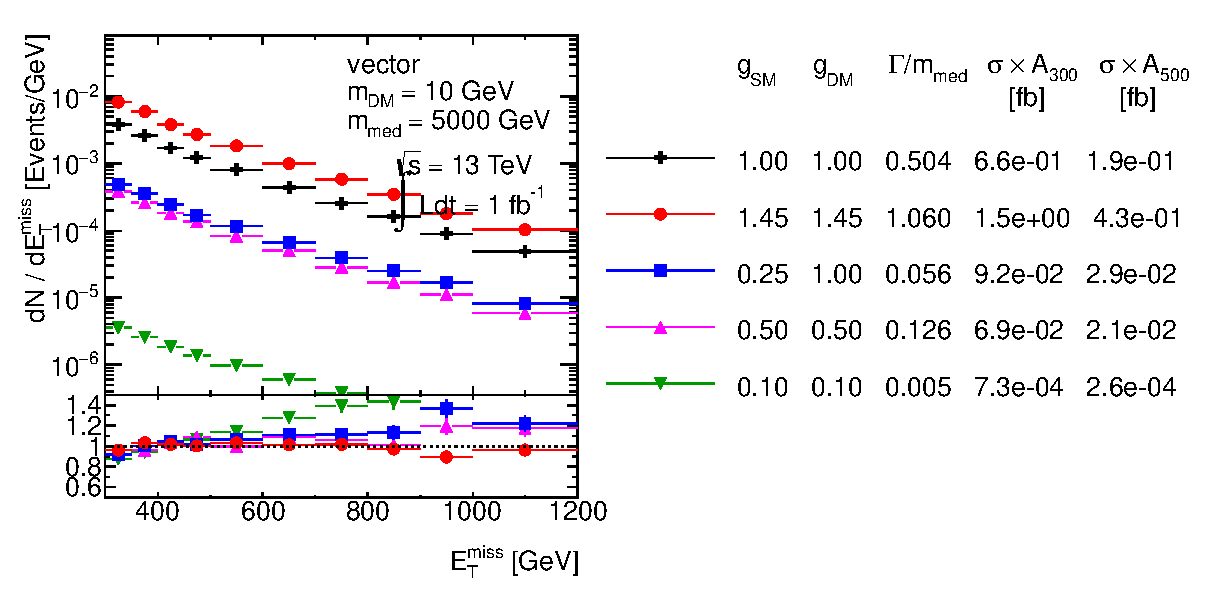
\includegraphics[width=0.95\textwidth]{figures/monojet/scan_g_V_10_5000.eps}
%\caption{Scan over couplings. The $\MET$ distribution is compared for the vector mediator models using the parameters as indicated. Ratios of the normalized distributions with respect to the first one are shown. $A_{300}$ and $A_{500}$ in the table denote the acceptance of the $\MET>300$~\gev and $\MET>500$~\gev cut, respectively.}
%\label{fig:monojet_narrow}
%\end{figure}

\begin{figure*}
\centering
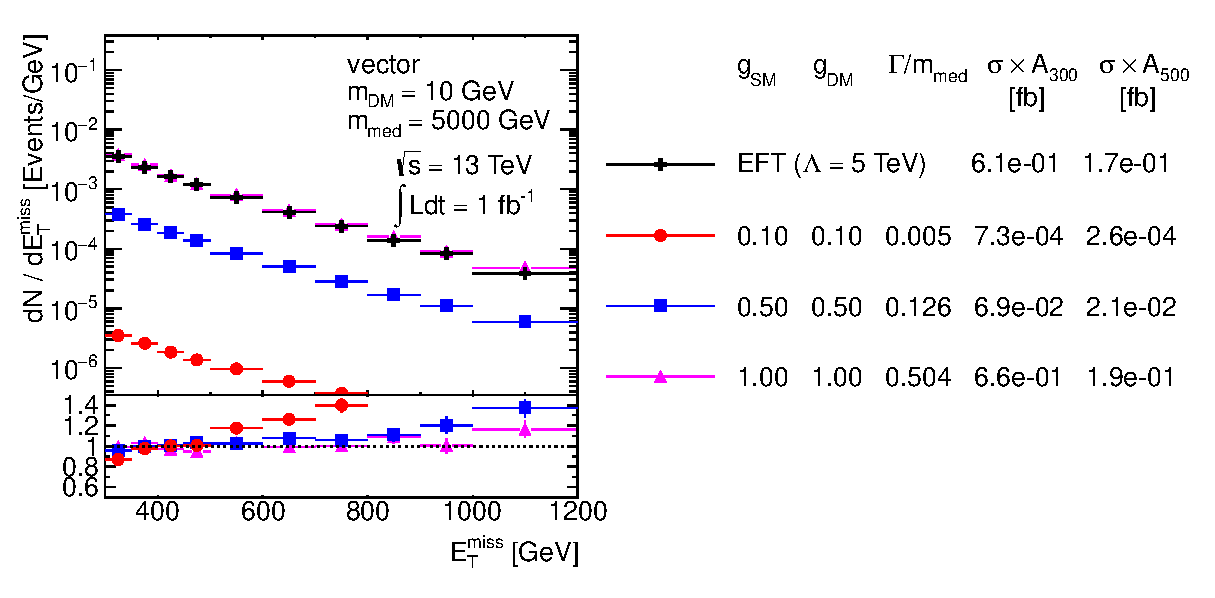
\includegraphics[width=0.95\textwidth]{figures/monojet/scan_g_EFT_10_5000.eps}
\caption[][-28pt]{Comparison of the $\MET$ distributions from the D5 EFT sample and the vector models with 5~\tev heavy mediator of various widths. Ratios of the normalized distributions with respect to the first one are shown. $A_{300}$ and $A_{500}$ in the table denote the acceptance of the $\MET>300$~\gev and $\MET>500$~\gev cut, respectively.}
\label{fig:monojet_narrow}
\end{figure*}

\begin{figure}
\centering
\subfloat[]{
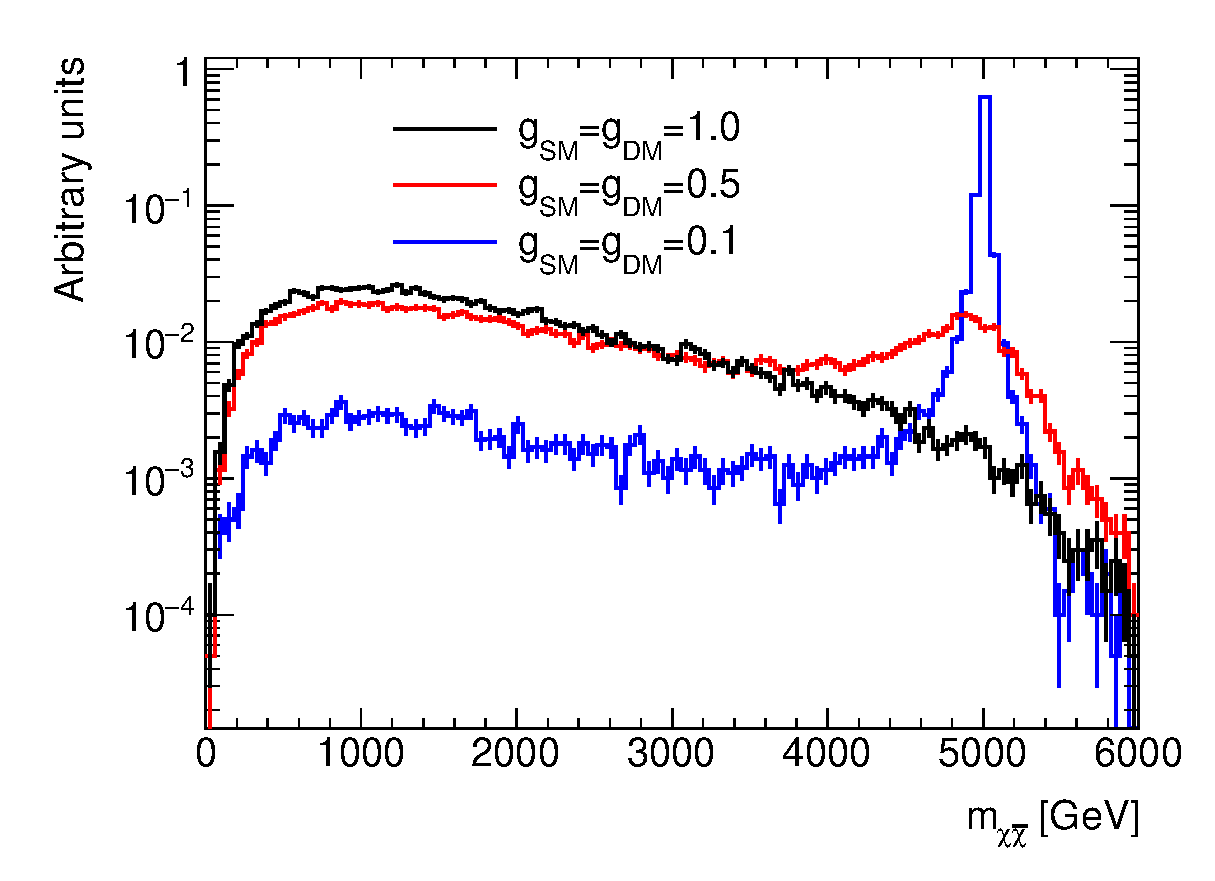
\includegraphics[width=0.8\textwidth]{figures/monojet/mxx.eps}% width = 0.73 => regular textwidth of figure environment. figure* used to avoid overlapping captions.
\label{fig:monojet_mchichi_a}}
\hfill
\subfloat[]{
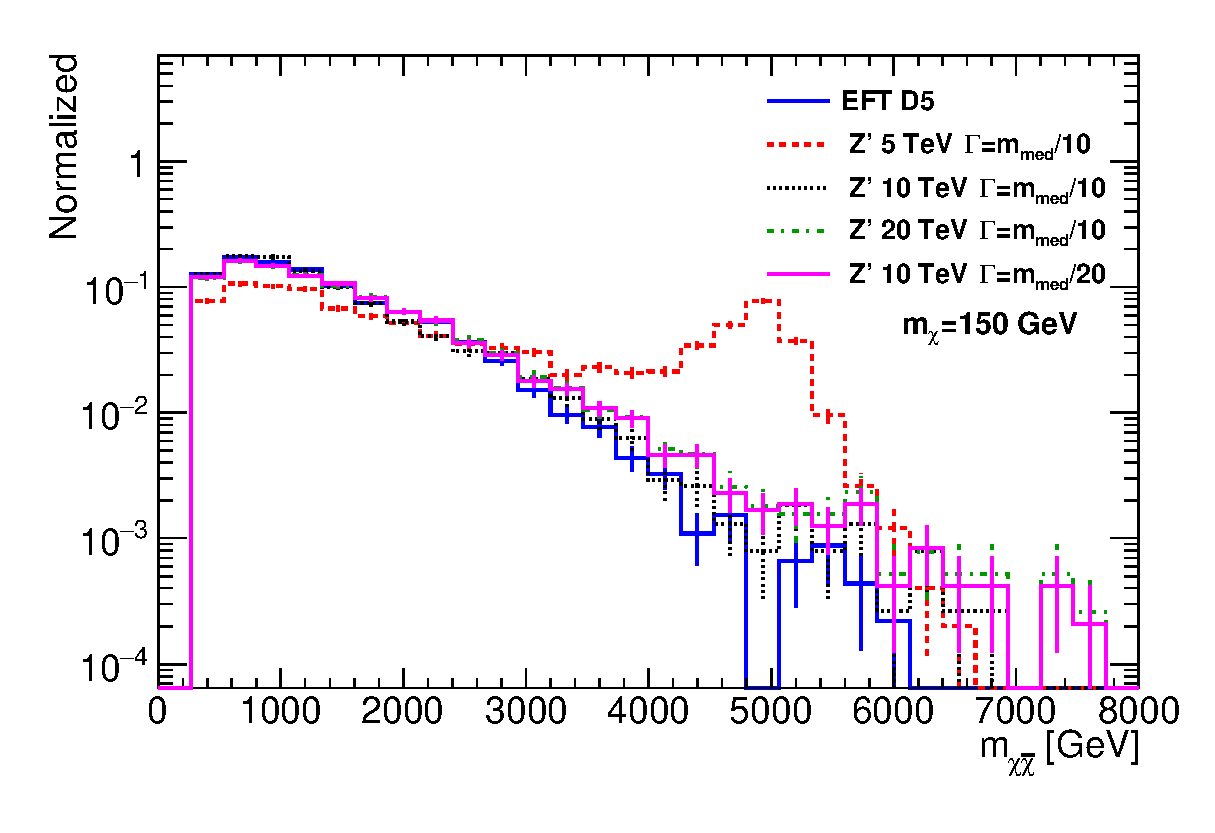
\includegraphics[width=0.8\textwidth]{figures/EFT/TruthShat3_compEFTvsZprime_DM150_narrow_new.eps}
\label{fig:monojet_mchichi_b}}
\caption[][14pt]{Invariant mass of the Dark Matter pair in the vector mediator samples with $\mDM=10$~\gev, $\mMed=5$~\tev and different coupling strengths (a).
Similar comparison is shown for the samples with different mediator masses considering $\Gamma_{\rm{min}}/\mMed=0.05$ and $0.1$ (b).
An EFT sample is also displayed in the latter case. The distributions are normalised to unit area.}
\label{fig:monojet_mchichi}
\end{figure}


Since kinematic distributions are robust to
changes in the specific values of coupling as long as heavy narrow mediators are generated correctly (see Appendix~\ref{thought:heavynarrowmediators} for discussion), 
the choice of $\gq=\gDM$ is reasonable 
to reduce the parameter space to be scanned. 
There are no complications associated
with small couplings, but, also, the early part of Run~2 will not be
sensitive to them.  The range of couplings we recommend limit the
calculated width of the mediator to be near or below \mMed.

For direct mediator searches, such as $q\bar q\to Z^\prime \to q\bar q$, asymmetric couplings ($\gq \ne \gDM$)
might also be considered. A scan in \gDM vs \gq can then be performed for a fixed mediator mass. Such searches
%such as those for
%dijet resonances,
may restrict \gq to a greater degree than
\gDM.

\subsubsection{Scan over \mDM}

For a fixed mediator mass \mMed and couplings, the Dark Matter mass falls into three regimes:
\begin{itemize}
\item[On-shell:] When $\Mmed \gg 2 \mDM$, most mediators are produced on-shell. The hardness of the ISR is set by \Mmed, and the kinematic distributions do not strongly depend on \mDM. This is illustrated in Fig.~\ref{fig:monojet_scan_V_mDM1000} for an example of \mMed=1~\tev 10~\gev $<\mDM<$ 300~\gev. The cross section decreases as the \mDM approaches $\mMed/2$. A coarse binning along $\mDM$ is sufficient.
\item[Threshold:] When $\Mmed \approx 2\mDM$, the production is resonantly enhanced, and both the cross section and kinematic distributions change more rapidly as a function of the two masses, and finer binning is needed in order to capture the changes.
\item[Off-shell:] When $\Mmed \ll 2 \mDM$, the Dark Matter pair is produced off-shell. The mediator propagator gives an explicit suppression of $(\Mmed/Q)^2$ that suppresses hard ISR. The $\mDM=1$~\tev case, shown in Fig.~\ref{fig:monojet_scan_V_mDM1000}, and Figure\,\ref{fig:monojet_scan_V_mDM100} demonstrates that the \MET spectrum hardens with increasing \mDM, accompanied by the gradual decrease of the cross section. Due to the significant cross section suppression, it is not necessary to fully populate the parameter space. Imminent LHC searches are not expected to be sensitive to these signals.
\end{itemize}

\begin{figure*}
\centering
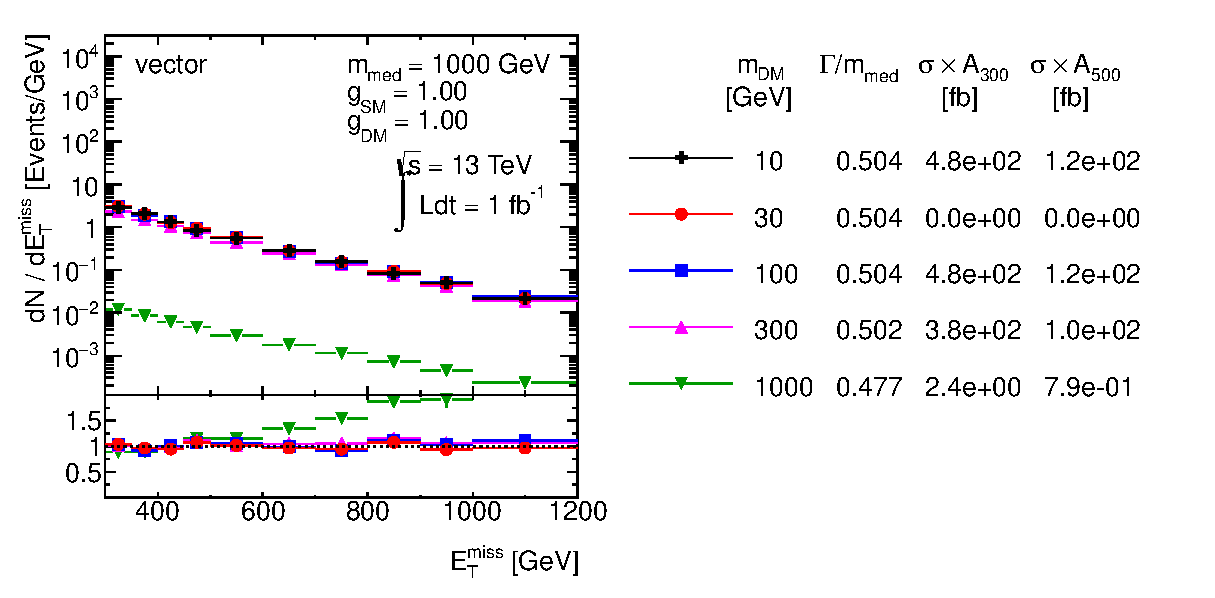
\includegraphics[width=0.95\textwidth]{figures/monojet/scan_mDM_V_1000.eps}
\vspace{4\baselineskip}
\caption[][-84pt]{Scan over Dark Matter mass. The $\MET$ distribution is compared for the vector mediator models using the parameters as indicated. Ratios of the normalized distributions with respect to the first one are shown. $A_{300}$ and $A_{500}$ in the table denote the acceptance of the $\MET>300$~\gev and $\MET>500$~\gev cut, respectively.}
\label{fig:monojet_scan_V_mDM1000}
\end{figure*}

\begin{figure*}
\centering
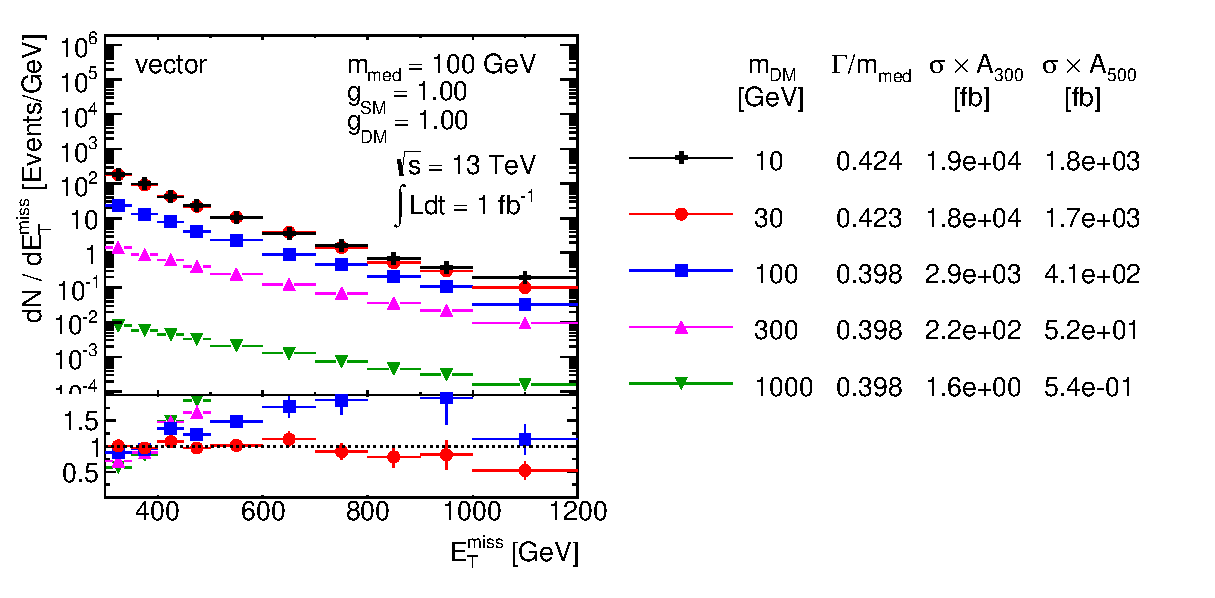
\includegraphics[width=0.95\textwidth]{figures/monojet/scan_mDM_V_100.eps}
\vspace{4\baselineskip}
\caption[][-84pt]{Scan over Dark Matter mass. The $\MET$ distribution is compared for the vector mediator models using the parameters as indicated. Ratios of the normalized distributions with respect to the first one are shown. $A_{300}$ and $A_{500}$ in the table denote the acceptance of the $\MET>300$~\gev and $\MET>500$~\gev cut, respectively.}
\label{fig:monojet_scan_V_mDM100}
\end{figure*}

\subsubsection{Scan over the mediator mass}

Changing the mediator mass for fixed Dark Matter mass and couplings leads to significant differences in cross section and shapes of the kinematic variables for on-shell production, as shown in Fig.\,\ref{fig:monojet_scan_V_mMed10}. As expected, higher mediator masses lead to harder $\MET$ spectra.
On the other hand, the $\MET$ shapes are similar in the off-shell Dark Matter production regime.  This
is illustrated in Fig.\,\ref{fig:monojet_scan_V_mMed1000}. Therefore, a coarse binning in \mMed is sufficient in the off-shell regime.

\begin{figure*}
\centering
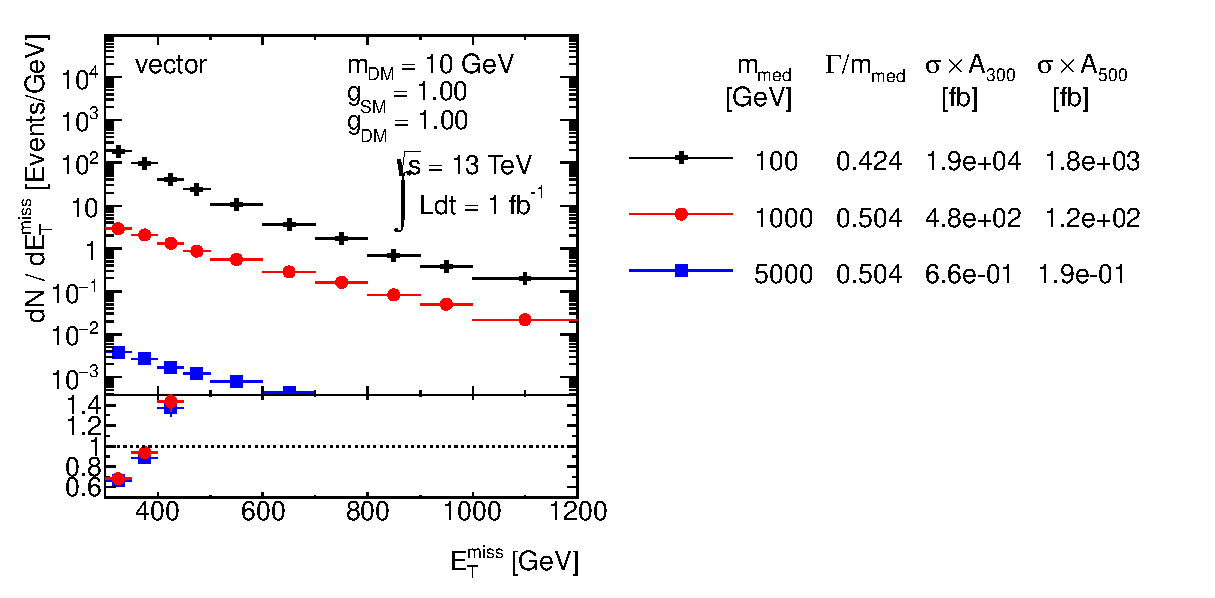
\includegraphics[width=0.95\textwidth]{figures/monojet/scan_mMed_V_10.eps}
\vspace{4\baselineskip}
\caption[][-84pt]{Scan over mediator mass. The $\MET$ distribution is compared for the vector mediator models using the parameters as indicated. Ratios of the normalized distributions with respect to the first one are shown. $A_{300}$ and $A_{500}$ in the table denote the acceptance of the $\MET>300$~\gev and $\MET>500$~\gev cut, respectively.}
\label{fig:monojet_scan_V_mMed10}
\end{figure*}

\begin{figure*}
\centering
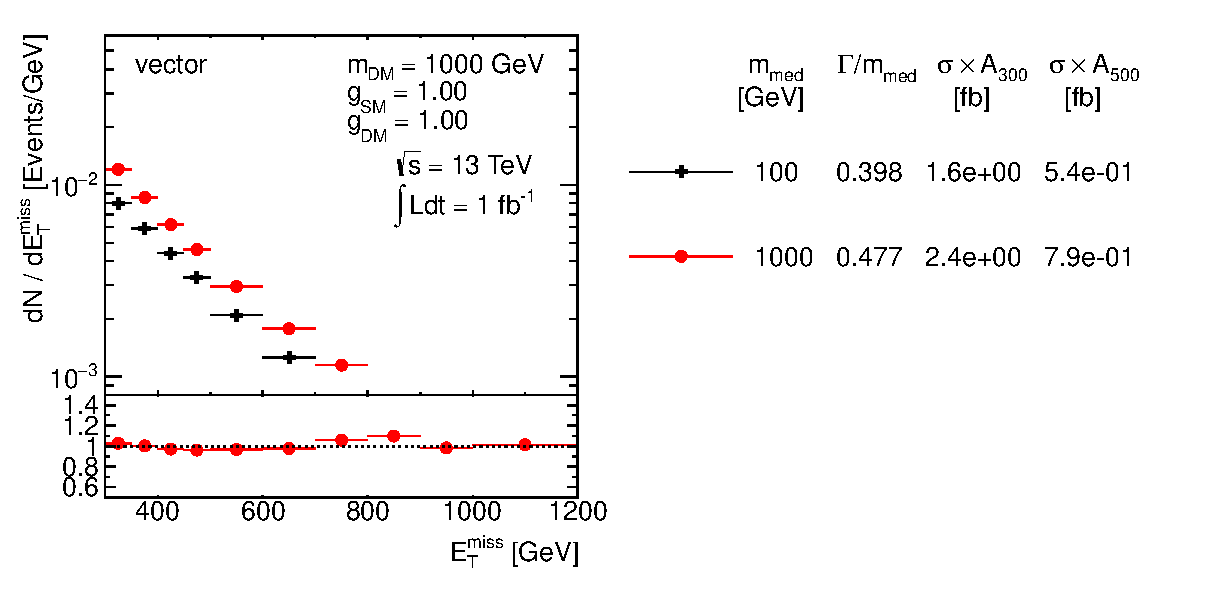
\includegraphics[width=0.95\textwidth]{figures/monojet/scan_mMed_V_1000.eps}
\caption[][-28pt]{Scan over mediator mass. The $\MET$ distribution is compared for the vector mediator models using the parameters as indicated. Ratios of the normalized distributions with respect to the first one are shown. $A_{300}$ and $A_{500}$ in the table denote the acceptance of the $\MET>300$~\gev and $\MET>500$~\gev cut, respectively.}
\label{fig:monojet_scan_V_mMed1000}
\end{figure*}

%% new section by DS, moved in parameter scan by CD
\subsubsection{Spin structure of the couplings}
\label{sec:monojet_spin}

This section compares the kinematic properties of vector, axial-vector and mixed vector/axial-vector models.
The samples with pure vector and pure axial-vector couplings are compared for $\mMed=100$~\gev and different 
Dark Matter masses in Fig.\,\ref{fig:monojet_VAmodels}. %The minimal width between the samples with the same Dark Matter and mediator masses differ only at the percent level.
No differences in the shape of the \MET distributions are observed between the samples with coincident masses. 
%\Todo{Do we want to propose to generate one model only and refer to the cross section tables in HEPData repository for the other?}
In the case of the on-shell Dark Matter pair production where $2\mDM\ll\mMed$, the cross sections of the pure vector and pure axial-vector models are similar. With increasing Dark Matter mass towards the $2\mDM=\mMed$ transition and beyond into the off-shell production regime, the relative difference between the cross sections of the two samples is increasing, with the vector samples having larger cross sections. 
%{This can be understood in the eikonal approximation since the A terms have an additional $v^2$ in front.}

\begin{figure*}
	\centering
	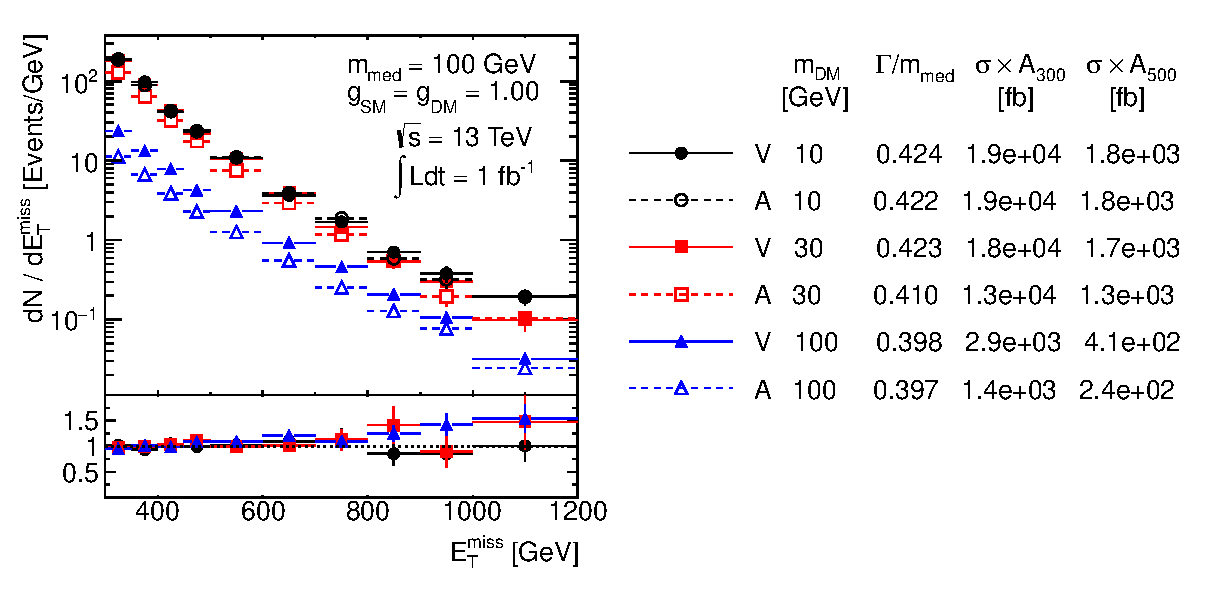
\includegraphics[width=0.95\textwidth]{figures/monojet/compareModels_VA_100.eps}
	\caption[][-28pt]{Comparison of the pure vector and pure axial-vector couplings. The $\MET$ distribution is shown for the samples generated with $\mMed=100$~\gev and different Dark Matter masses. Ratios of the normalized distributions are shown for between the samples with coincident masses. $A_{300}$ and $A_{500}$ in the table denote the acceptance of the $\MET>300$~\gev and $\MET>500$~\gev cut, respectively.}
	\label{fig:monojet_VAmodels}
\end{figure*}

Figure\,\ref{fig:monojet_scan_VA_mMed1000} shows the samples generated with pure and mixed couplings for $\mDM=100$~\gev and $\mMed=1\,\tev$, i.e. where the Dark Matter pair is produced on-shell. The mediator width between the pure vector and pure axial-vector couplings differ only by 2\% in this case, and $<10\%$ agreement between the cross sections is found. The mediator widths for the samples with the same type coupling to quarks agree at better than 1\% since the width is dominated by the quark contribution, as expected from
Eq.\,\ref{eq:monojet_min}.
%In the mediator rest frame, the angular distribution of the DM relative to the mediator direction of motion has the form $1+z^2+2*C*z$, where $z=\cos\theta$, with the second term only present in the mixed case, which may lead to acceptance differences.
No significant differences between the samples with same type Dark Matter coupling are seen, given the statistical precision of the generated samples. This is expected since the mediator is produced on-shell, and the details of the invisible decay are unimportant in cut-and-count searches.

For the off-shell Dark Matter pair production, shown in Fig.\,\ref{fig:monojet_scan_VA_mMed100} for $\mDM=100$~\gev and $\mMed=100$~\gev,
there is approximately a factor 2 difference
between the cross-sections of the samples with pure couplings is observed. As in the previous case, the samples with the same type coupling to Dark Matter are similar both in terms of cross sections and \MET shape. Since the contribution to the mediator width from Dark Matter is closed in this case, only the quark couplings define the width. Only couplings to light quarks are opened in the case of $\mMed=100$~\gev for which the differences between the partial widths of vector and axial-vector couplings are marginal. This explains the similar minimal widths for all four samples stated in Fig.\,\ref{fig:monojet_scan_VA_mMed100}.

In general, the coupling to quarks is not expected to play an important role in the kinematics as it is only needed to produce the mediator which is confirmed by the observations above. 
%For scalar and pseudoscalar mediators, the coupling to Dark Matter determines the form of the matrix element which explains the similarity of the samples with the same type Dark Matter couplings. 
Based on this argument and on the observations above, we recommend to consider only the models with pure vector couplings or pure axial-vector couplings for simulation.

\begin{figure*}
	\centering
	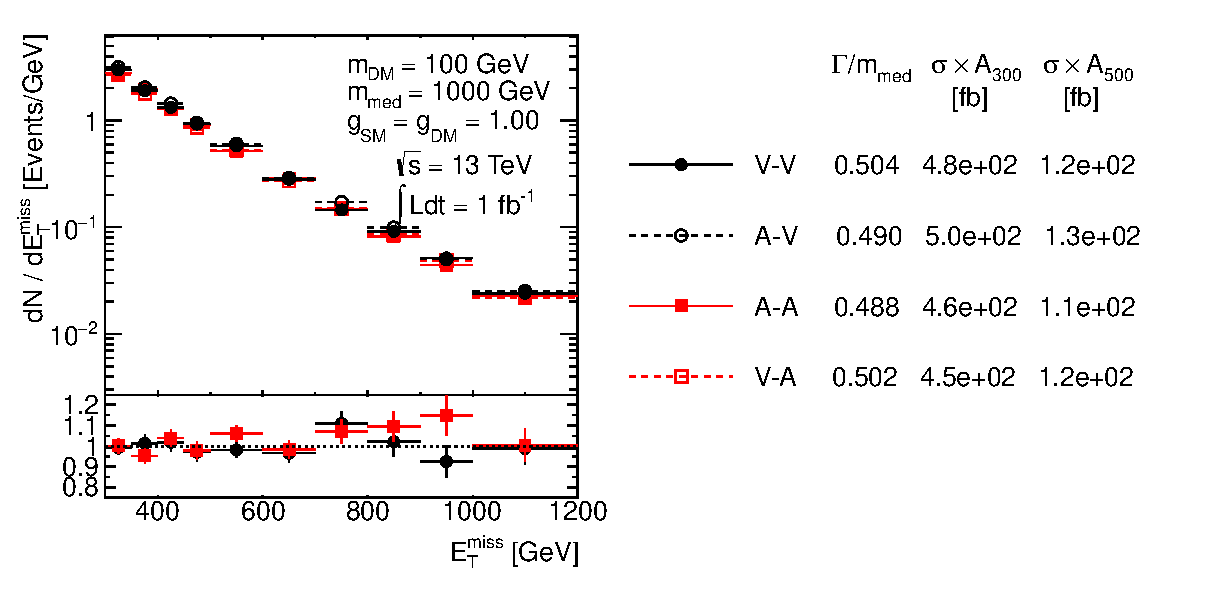
\includegraphics[width=0.95\textwidth]{figures/monojet/compareVA_100_1000.eps}
	\caption[][-28pt]{Comparison of the pure vector, V-V, and pure axial-vector, A-A, couplings with mixed couplings, A-V and V-A where the first (second) letter indicates the Standard Model (Dark Sector) vertex. The $\MET$ distribution is shown for the samples generated with $\mDM=100$~\gev and $\mMed=1$~\tev. Ratios of the normalized distributions are shown for A-V over V-V and for V-A over A-A. $A_{300}$ and $A_{500}$ in the table denote the acceptance of the $\MET>300$~\gev and $\MET>500$~\gev cut, respectively.}
	\label{fig:monojet_scan_VA_mMed1000}
\end{figure*}

\begin{figure*}
	\centering
	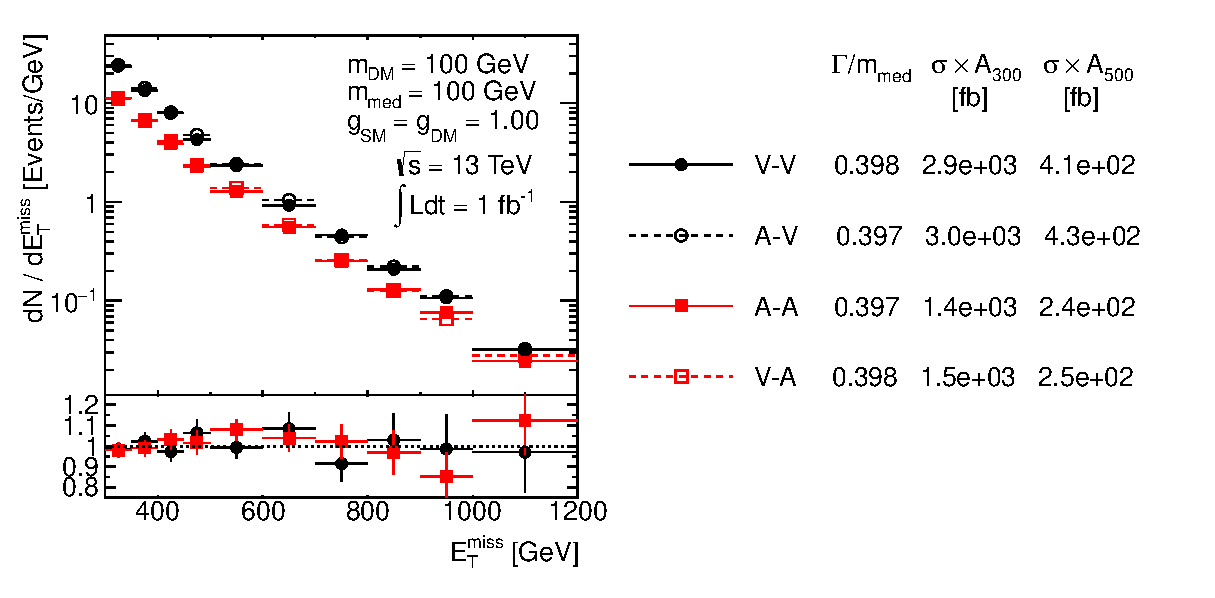
\includegraphics[width=0.95\textwidth]{figures/monojet/compareVA_100_100.eps}
	\caption[][-28pt]{Comparison of the pure vector, V-V, and pure axial-vector, A-A, couplings with mixed couplings, A-V and V-A where the first (second) letter indicates the Standard Model (Dark Sector) vertex. The $\MET$ distribution is shown for the samples generated with $\mDM=100$~\gev and $\mMed=100$~\gev. Ratios of the normalized distributions are shown for A-V over V-V and for V-A over A-A. $A_{300}$ and $A_{500}$ in the table denote the acceptance of the $\MET>300$~\gev and $\MET>500$~\gev cut, respectively. The suppression by $\beta^3$ for $\mDM\sim\mMed$ can be seen for the curves representing axial DM coupling.}
	\label{fig:monojet_scan_VA_mMed100}
\end{figure*}
%%% end of the new section by DS

\subsubsection{Proposed parameter grid}

The final step in proposing a parameter grid is to evaluate the sensitivity
of Run-2 LHC data with respect to rate and/or kinematics.
%In order to motivate the highest mediator mass grid point, the expected sensitivity of Run-2 LHC data needs to be taken into account.
The parameter scan focuses on two important regions, the light mediator region and  the heavy mediator limit to reproduce the EFT limit, 
and takes into account the projected sensitivities for the mono-jet analysis.

Considering simplified models also allows to discuss constraints from different search channels. In the case of the \schannel exchange, the results from the mono-jet final states, where the mediator decays to a DM pair, one can also take into account dijet constraints on the processes where the mediator decays back to Standard Model particles. The importance of the dijet results depend on the magnitude of the coupling $\gq$. We recommend to keep the two channels rather independent by choosing $\gq=0.25$ and $\gDM=1$, based on the findings given in Ref.\,\cite{Chala:2015ama}. Furthermore, it is also important to mention this choice leads to $\Gamma_{\rm{min}}/\mMed \lsim 0.06$. Note that the usual choice of $\gq=\gDM=1$ used in literature leads to $\Gamma_{\rm{min}}/\mMed \sim 0.5$, questioning the applicability of the narrow width approximation.

Projected sensitivities for a 14~\tev\, mono-jet analysis are available from ATLAS~\cite{ATL-PHYS-PUB-2014-007}. The expected upper limit at 95\% confidence level on the product of cross section, acceptance and efficiency, $\sigma\times A\times\epsilon$, in the final Run-1 ATLAS mono-jet analysis\,\cite{Aad:2015zva} is 51\,fb and 7.2\,fb  for $\MET>300$~\gev and $\MET>500$~\gev, respectively. These ATLAS studies estimate a factor of two increase in sensitivity with the 2015 data. Given that cross section for $W/Z+$jets processes increases by roughly a factor 2 %\Todo{Can we get more precise number and a citation? Is this in Sarah's V+jets paper?} 
when going from $\sqrt{s}=8$~\tev to 13~\tev, similar fiducial cross section limits can be expected with the first Run-2 data as from the final Run-1 analysis.
The generator level cross section times efficiency times acceptance at $\MET>500$~\gev for the model with couplings $\gq=0.25$ and $\gDM=1$, a light Dark Matter particle of
\mDM=10~\gev and a \mMed=1~\tev vector mediator is at the order of 100\,fb, i.e. the early Run-2 mono-jet analysis is going to be sensitive to heavier mediators than this. The value of $\sigma\times \epsilon \times A$ at $\MET>500$~\gev for a 5~\tev vector mediator is at the order of 0.1\,fb, therefore this model lies beyond the reach of the LHC in the early Run-2. However, models with high enough mediators are still useful to reproduce the EFT result.

Following these arguments, \mMed grid points are chosen, roughly equidistant in a logarithmic scale: 10~\gev, 20~\gev, 50~\gev,  100~\gev, 200~\gev, 300~\gev, 500~\gev, 1000~\gev and 2000~\gev. In the threshold regime $\mMed=2\mDM$, the $\mDM$ grid points are taken at approximately $\mMed/2$, namely: 10~\gev, 50~\gev, 150~\gev, 500~\gev and 1000~\gev. Points on the on-shell diagonal are always chosen to be 5~\gev away from the threshold, to avoid numerical instabilities in the event generation. 
The detailed studies of the impact of the parameter changes on the cross section and kinematic distributions presented earlier in this section support removing some of the grid points and relying on interpolation. The optimized grids proposed for the vector and axial-vector mediators are given in Table.\,\ref{tab:mDMmMedScan_VA}.
% containing 36
%29 
%mass points each. 
One point at very high mediator mass (10~\tev) is added for each of the DM masses scanned, to aid the reinterpretation of results in terms of contact interaction operators (EFTs), as discussed in Section~\ref{sec:RecommendationEFTResults}. 

% \begin{figure}
% \centering
% 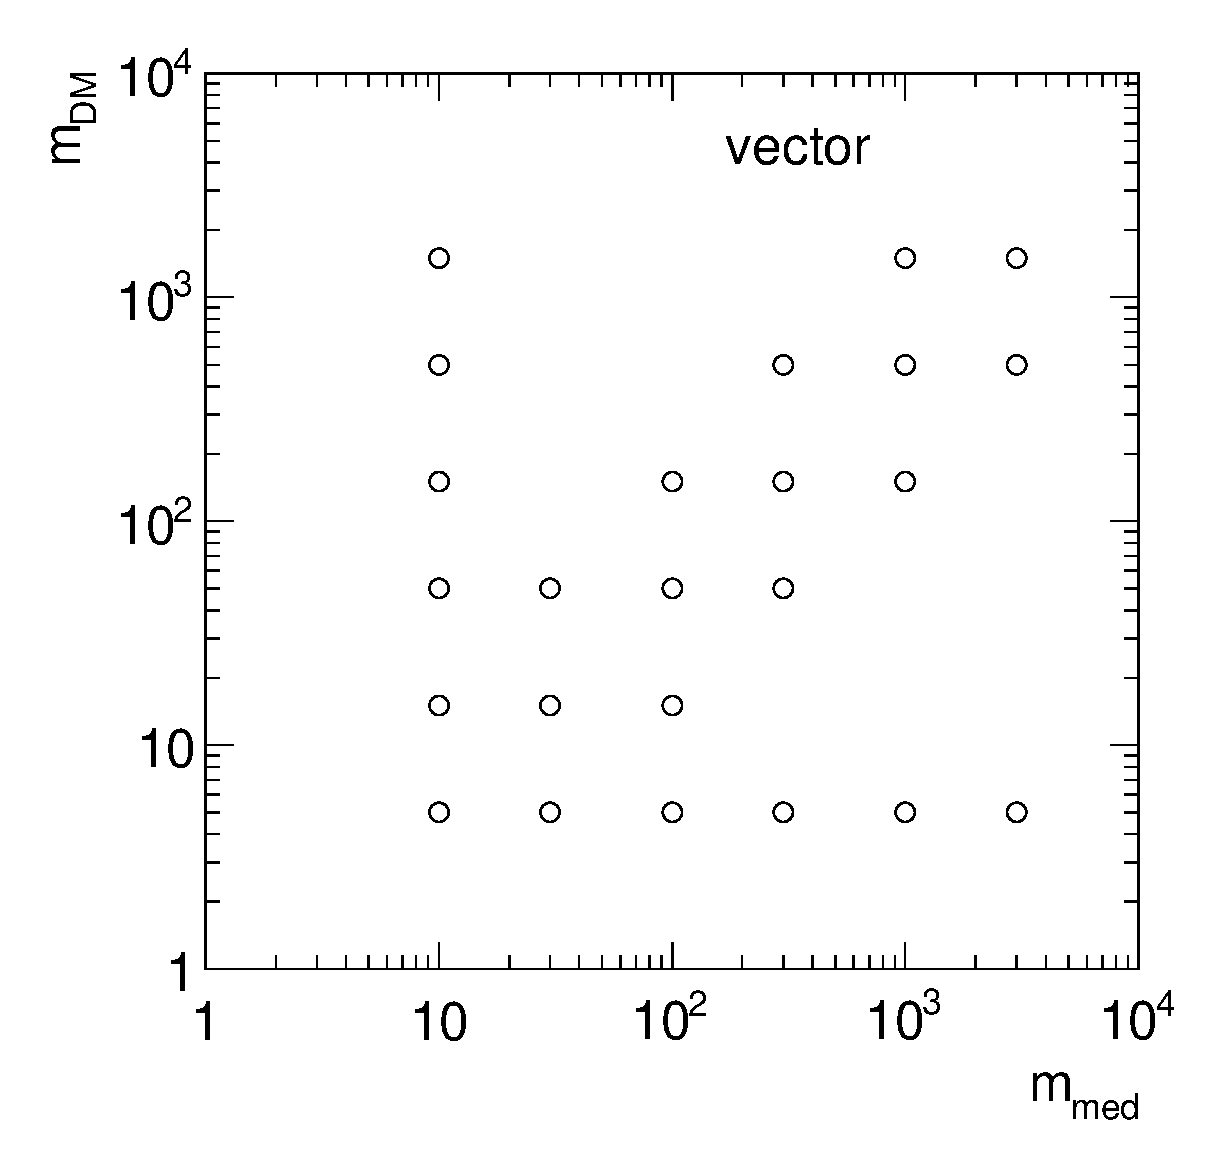
\includegraphics[width=0.95\textwidth]{figures/monojet/grid_V.eps}
% 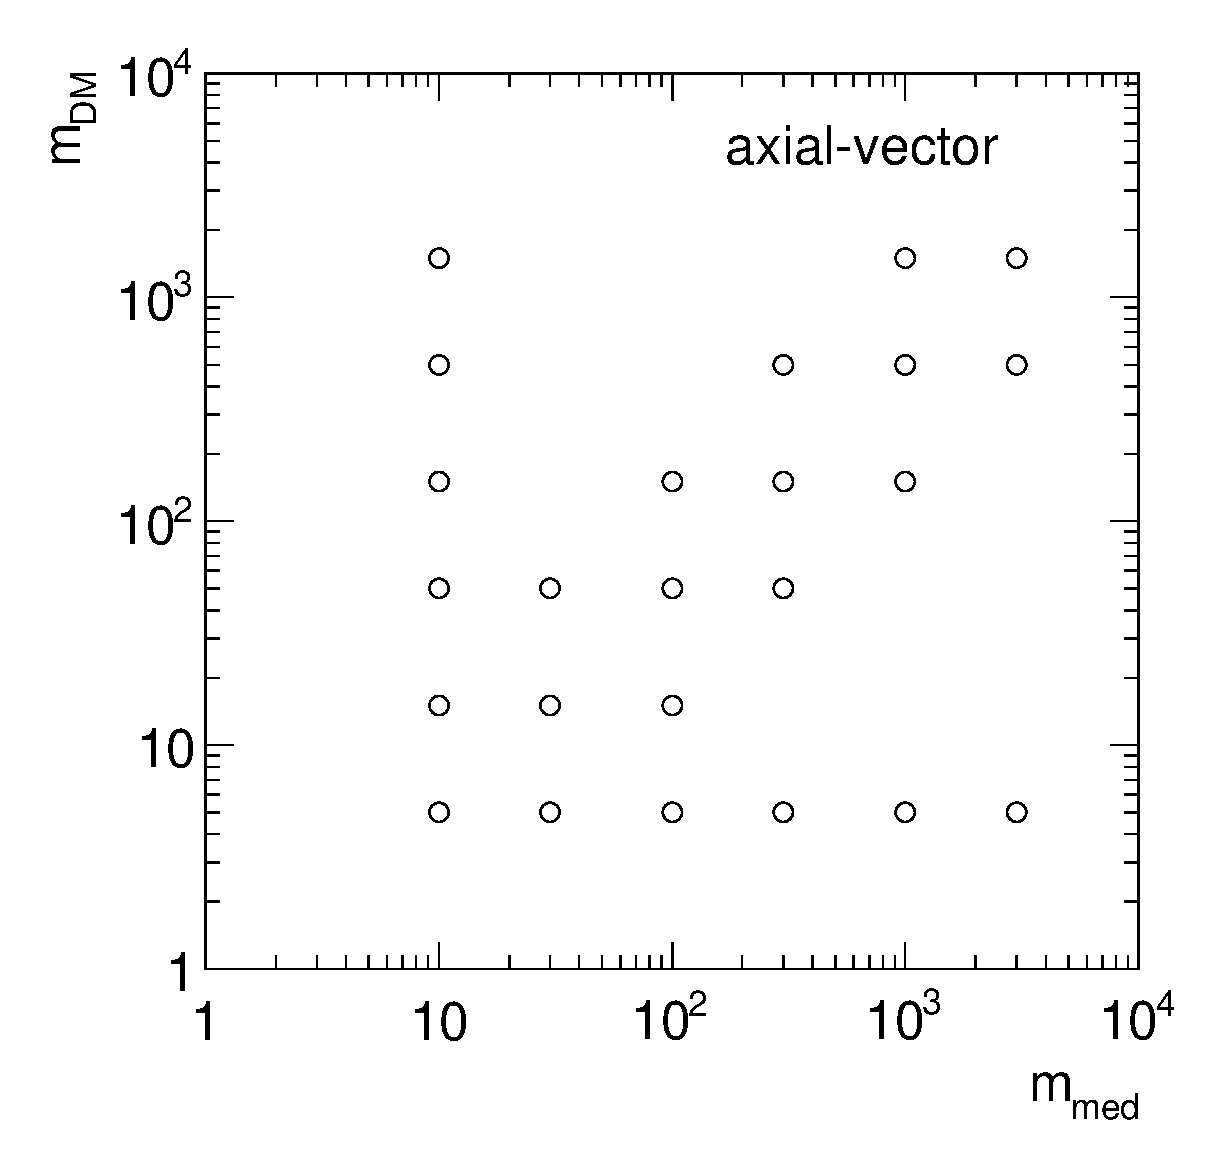
\includegraphics[width=0.95\textwidth]{figures/monojet/grid_A.eps}
% \caption{Proposed parameter grid for vector and axial-vector mediator in the $\mMed$--$\mDM$ plane.}
% \label{fig:monojet_grid_V}
% \end{figure}

\begin{table}[!h]
\centering
\resizebox{\textwidth}{!}{
\begin{tabular}{| l |r r r r r r r r r r|}
\hline
\multicolumn{1}{|c|}{\mDM/\gev} & \multicolumn{10}{c|}{\mmed/\gev} \\
\hline
 1             &         10  & 20 & 50 & 100 & 200 & 300 & 500 &         1000  &                 2000   &         10000  \\
 10   	       &         10  & 15 & 50 & 100 &     &     &     &               &                        &     10000      \\
 50            &   10  & 
& 50 &  95 & 200 & 300 &     &               &                        &    10000       \\
 150           &         10  &    &    &     & 200 & 295 & 500 &    1000    &                  &     10000      \\
 500           &         10  &    &    &     &     &     & 500 &          995  &                 2000   &     10000      \\
 1000          &         10  &    &    &     &     &     &     &         1000  &                 1995   &         10000  \\
\hline
\end{tabular}
}
\caption{Simplified model benchmarks for \schannel simplified models (\spinone mediators 
decaying to Dirac DM fermions in the V and A case, taking the minimum width for \gq = 0.25 and \gDM = 1)}.
% Points in \textbf{bold} are only generated for the vector/axial vector cases, while points in 
% \textit{italics} are generated for the monojet analysis 
% but not for the search including heavy quarks. This table corresponds to 29 points for monojet vector/axial vector models,
% 26 points for monojet scalar/pseudoscalar models and 24 points for $t \bar{t}$+\MET scalar/pseudoscalar models.}

\label{tab:mDMmMedScan_VA}
% \end{sidewaystable}
\end{table}

%The presentation of the results in the $\gq$--$\gDM$ plane for fixed masses benefits from cross section scaling and is discussed in Section\,\ref{sec:monojet_scaling}.

%% It is difficult to visualize a four dimensional scan.
%% However, it is convenient to study the parameter dependence,
%% and present results, in two projections:
%% (a) the $\mMed$--$\mDM$ plane for a particular choice of the couplings, and\\
%% (b) the $\gq$--$\gDM$ plane for a particular choice of the masses.

%% %discuss expected sensitivity (cite PUB note) when motivating mDM and mMed range
%% %motivate the mass point for the coupilng scan
%% We choose to display the results in the $\mMed$--$\mDM$ plane for the choice of the couplings $\gq=\gDM=1$. 


Tables\,\ref{tab:widthV} and \ref{tab:widthA} give the $\Gamma_{\rm{min}}/\mMed$ ratio for the parameter grid proposed for vector and axial-vector \schannel models, respectively. The numbers range from $\sim0.02$ in the off-shell Dark Matter production regime at $2\mDM>\mMed$ to $\sim0.06$ in the on-shell regime for heavy mediators where all coupling channels contribute.

\begin{table}
	\centering
	\resizebox{\textwidth}{!}{
		\begin{tabular}{| l |r r r r r r r r r r|}
			\hline
			\multicolumn{1}{|c|}{\mDM/\gev} & \multicolumn{10}{c|}{\mmed/\gev} \\
			&         10  & 20 & 50 & 100 & 200 & 300 & 500 &         1000  &                 2000   &         10000  \\
			\hline
			\hline
			1 & 0.049  & 0.051  & 0.051  & 0.051  & 0.051  & 0.051  & 0.056  & 0.056  & 0.056  & 0.056  \\
			10 & 0.022  & 0.024  & 0.054  & 0.052  &        &        &        &        &        & 0.056  \\
			50 & 0.022  &        & 0.025  & 0.025  & 0.055  & 0.053  &        &        &        & 0.056  \\
			150 & 0.022  &        &        &        & 0.025  & 0.025  & 0.061  & 0.058  &        & 0.056  \\
			500 & 0.022  &        &        &        &        &        & 0.029  & 0.030  & 0.060  & 0.057  \\
			1000 & 0.022  &        &        &        &        &        &        & 0.030  & 0.030  & 0.057  \\
			\hline
		\end{tabular}}
		\caption%[][5cm]
		{Minimal width of the vector mediator exchanged in \schannel divided by its mass, assuming $\gq=0.25$ and $\gDM=1$. The numbers tabulated under $2\mDM=\mMed$ correspond to the width calculated for $\mMed-5$~\gev.}
		\label{tab:widthV}
	\end{table}
	\vspace{4cm}
	
	\begin{table}
		\centering
		\resizebox{\textwidth}{!}{
			\begin{tabular}{| l |r r r r r r r r r r|}
				\hline
				\multicolumn{1}{|c|}{\mDM/\gev} & \multicolumn{10}{c|}{\mmed/\gev} \\
				&         10  & 20 & 50 & 100 & 200 & 300 & 500 &         1000  &                 2000   &         10000  \\
				\hline
				\hline
				1 & 0.045  & 0.049  & 0.051  & 0.051  & 0.051  & 0.051  & 0.053  & 0.055  & 0.056  & 0.056  \\
				10 & 0.020  & 0.022  & 0.047  & 0.050  &        &        &        &        &        & 0.056  \\
				50 & 0.020  &        & 0.025  & 0.025  & 0.045  & 0.048  &        &        &        & 0.056  \\
				150 & 0.020  &        &        &        & 0.025  & 0.025  & 0.044  & 0.053  &        & 0.056  \\
				500 & 0.020  &        &        &        &        &        & 0.027  & 0.029  & 0.050  & 0.056  \\
				1000 & 0.020  &        &        &        &        &        &        & 0.029  & 0.030  & 0.055  \\
				\hline
			\end{tabular}}
			\caption%[][5cm]
			{Minimal width of the axial-vector mediator exchanged in \schannel divided by its mass, assuming $\gq=0.25$ and $\gDM=1$. The numbers tabulated under $2\mDM=\mMed$ correspond to the width calculated for $\mMed-5$~\gev.}
			\label{tab:widthA}
		\end{table}
		\vspace{4cm}

\subsection{Additional considerations for $V$+\MET{} signatures}
\label{sec:bosonrad}
\svnidlong
{$HeadURL: $}
{$LastChangedDate: $}
{$LastChangedRevision: $}
{$LastChangedBy: $}
\svnid{$Id: $}   

All models detailed in this Section are applicable to signatures where 
 a photon, a W boson, a Z boson or a Higgs boson
 is radiated from the initial state partons instead of a gluon. 
The experimental signature is identified as \textit{V+\MET} and it
has been studied in Refs.~\cite{}.

\Todo{Add experimental citations.}
\Todo{Add link to section describing EW bosons from a blob. CD: why here?}

Monojet searches are generally more sensitive
with respect to final states including bosons, due to the much
larger rates of signal events featuring quark or gluon radiation with
respect to radiation of bosons~\cite{Zhou:2013fla},
in combination with the low branching ratios if leptons from
boson decays are required in the final state.
The rates for the Higgs boson radiation is too low for these models
to be considered a viable benchmark~\cite{Carpenter:2013xra}.
However, the presence of photons,
leptons from W and Z decays,
and W or Z bosons decaying hadronically
allow backgrounds to be rejected more effectively,
making Z/gamma/W+\MET searches
still worth comparing with searches in the jet+\MET final state.

%\Todo{Additional motivations exist for this final state from SUSY searches.}
%TODO: Linda is writing sentence to make this stronger. 

% The three commonly chosen EFT benchmarks for Dirac dark matter that are
% kinematically distinct for what concerns the observables used in
% \MET+X searches~\footnote{[CD: we would need a plot here, or a reference to
% monojet section where this is shown]} and span a wide range of \MET spectrum in
% the boson+\MET searches are, in the notation of ~\cite{Goodman:2010ku},
% the D1 (scalar SM/WIMP interaction), D5 (vector-vector interaction) and D9
% (tensor interaction) operator.

In the case of a spin-1 mediator,
an example Feynman diagram for these processes can be constructed by taking
Fig.~\ref{fig:OP} and replacing the gluon with $\gamma,W$ or $Z$.
The interest for searches with W bosons in the final state
has been elevated by the increased cross section
for certain choices of couplings for a spin-1 mediator~\cite{Bai:2012xg}.
Run-1 searches have considered three sample cases for the product of
up and down quark couplings to the mediator, denoted as $\xi$:
\begin{itemize}
 \item[$\xi=0$:] Mediator couples to up-type or down-type quarks, but not both;
 \item[$\xi=1$:] Mediator couples to up-type and down-type quarks with same strength;
 \item[$\xi=-1$:] Mediator couples to up-type and down-type quarks with same strength, but opposite sign.
\end{itemize}
The $\xi=-1$ case leads to a large increase in the cross-section of the process,
and modifies the spectrum of missing transverse energy or
transverse mass used for the searches. The sensitivity of the W+\MET search for
this benchmark in this case surpasses that of the jet+\MET search.
However, as shown in Ref.~\cite{Bell:2015sza}, the cross-section increase is due
to the production of longitudinally polarized W bosons,
in violation of electroweak gauge symmetries. Unless further
particles are introduced (in a fashion similar
to the Higgs boson in the Standard Model), choosing a value of $\xi=-1$
for this simplified model will lead to a manifest violation of unitarity at LHC energies.
The simplified model with a vector mediator exchanged in the \schannel model
can still be considered as a benchmark for searches with a W boson if $\xi=1$.
We leave the study of further models with cross-section enhancements due
to different couplings to up and down quarks for studies beyond the early LHC searches
covered in this document.
An example of such model is the case of both DM and SM Higgs charged under a new $U(1)'$ symmetry,
with a  small mass mixing between the SM Z-boson and the new \Zprime-boson.
This leads
to different effective DM couplings to $u_L$ and $d_L$, proportional to
their coupling to the Z boson, detailed in Appendix~\ref{app:EWSpecificModels_Appendix}.


%The scan in the parameters that characterize this simplified model for EW boson + \MET
%searches follow what is
%already detailed in Section~\ref{subsec:MonojetLikeModels}.


% CD: I tend to like this list so I'll leave it here in hope of recycling it
% \begin{itemize}
%  \item the mass of the DM particle ($m_{DM}$);
%  \item the mediator mass ($m_{Med}$);
%  \item the mediator width ($\Gamma_{Med}$);
%  \item the couplings between the DM and the mediator (\gdm),
%  and between the mediator and the initial state quarks ($g_{SM}$);
%  \item the chirality of the couplings between DM and mediator,
%  and between mediator and initial state quarks (vector-vector, axial-vector, axial-axial, vector-axial).
% \end{itemize}

As in the case of the jet+\MET models, the width does not have a significant
impact on the kinematic distributions relevant for those searches. An example
of the particle-level analysis acceptance using the
generator-level cuts from Ref.~\cite{Aad:2014tda}
for the photon+\MET analysis, but raising the photon $p_T$ cut
to 150~\gev, is shown in Figure~\ref{fig:DMV_EW_gamma_acceptance},
comparing a width that is set to $\Gamma=M_{med}/3$ to the
minimal width (the ratio between the two widths
ranges from 1.05 to 1.5 with increasing mediator masses).

%% Redone as a table.
% mmed : minW
% 10  : 3.5
% 50 : 21.3
% 100 : 42.4
% 300 : 127.3
% 600 : 300.1
% 1000 : 503
% 3000 : 1512
% 6000 : 3024
\begin{table}[!h]
\begin{tabular}{| l |r r r r|}\hline
\multicolumn{5}{|c|}{Acceptance ratio for $\Gamma=\Gamma_{\rm min}$ vs
$\Gamma=\mMed/3$} \\ \hline 
\multicolumn{1}{|c|}{ } & \multicolumn{4}{c|}{\mdm/GeV}\\
\hline 
{\mMed/GeV}      & 10     & 50    & 200   & 400  \\ \hline
50   & 0.96   & 0.99  &       & 0.95 \\  
100  & 0.97   &       &       &      \\
300  & 1.00   & 1.02  &       &      \\
600  &        &       & 0.96  &      \\
1000 & 1.01   & 1.02  & 1.03  &      \\
3000 & 1.02   & 1.03  &       & 1.01 \\
\hline
\end{tabular}
    \caption{Analysis acceptance ratios for the photon+\MET analysis when varying the mediator width, in the
    case of a vector mediator exchanged in the $s-$channel}%This plot will come from Marie-Helene
    \label{fig:DMV_EW_gamma_acceptance}
\end{table}

%% \begin{figure}
%%     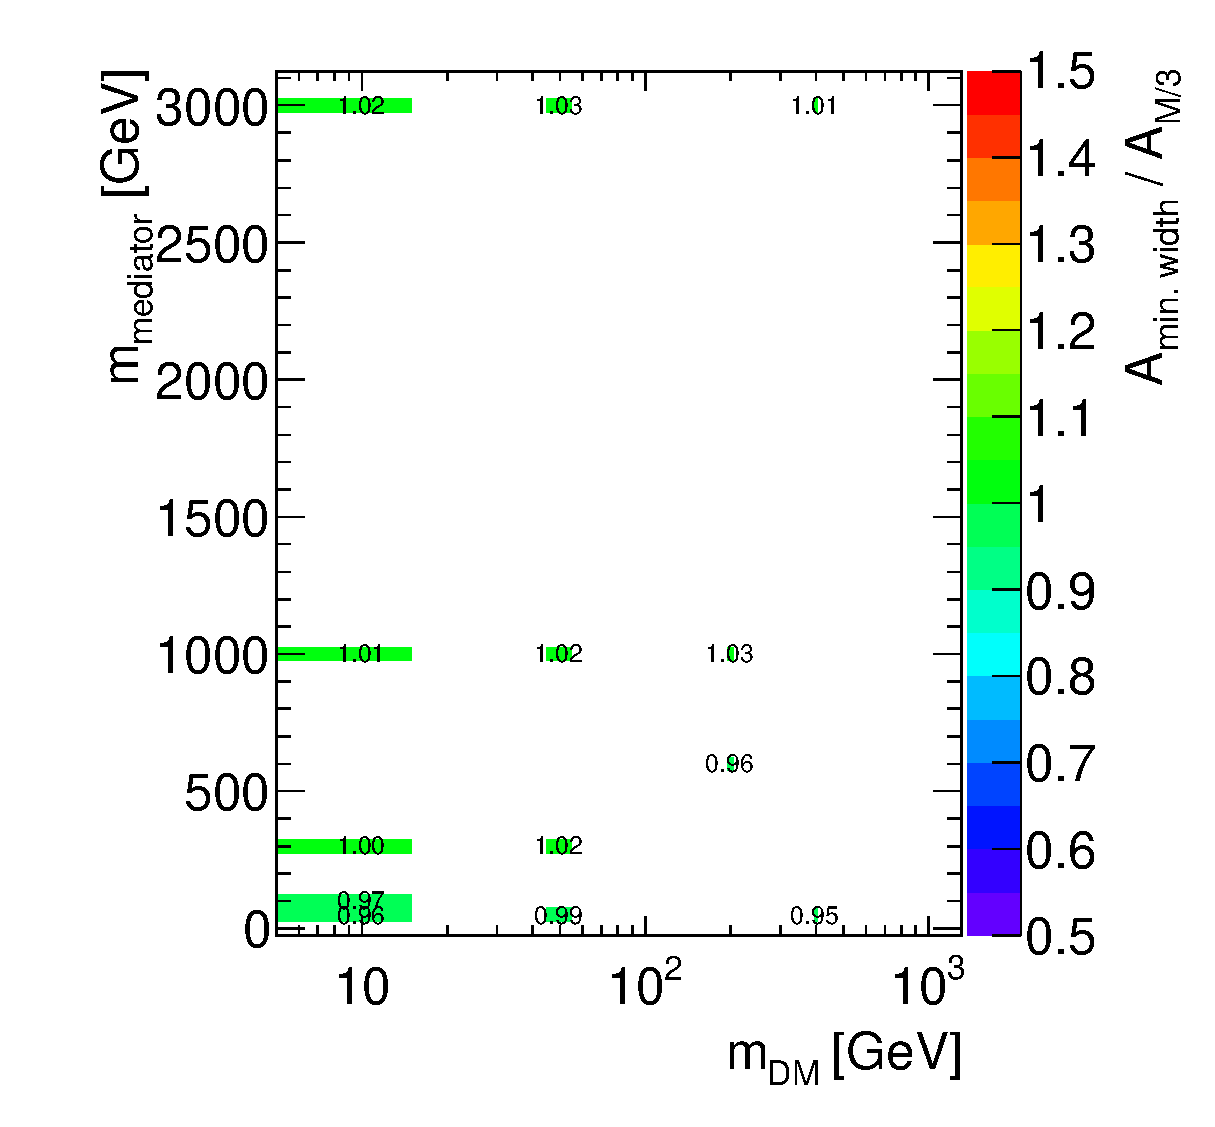
\includegraphics[width=0.7\textwidth]{figures/EW/acceptance_minwidth_vs_mo3_gamma}
%%     \caption{Analysis acceptance for the photon+\MET analysis when varying the mediator width, in the
%%     case of a vector mediator exchanged in the $s-$channel}%This plot will come from Marie-Helene
%%     \label{fig:DMV_EW_gamma_acceptance}
%% \end{figure}

Examples of relevant kinematic distributions for selected benchmark points are
shown in Fig.~\ref{fig:DMV_EW_kinematics_SVMed}. 
leading-order cross-sections for the chosen 
benchmark points are shown in Appendix~\ref{app:EWSpecificModels_Appendix}.

\begin{figure}[h!]
\centering  
\subfloat[Missing transverse momentum distribution for the photon+\MET final state, for 
different mediator mass choices, for \mdm=10~\gev.\label{fig:DMV_EW_gamma_MET_SVMed}]{%
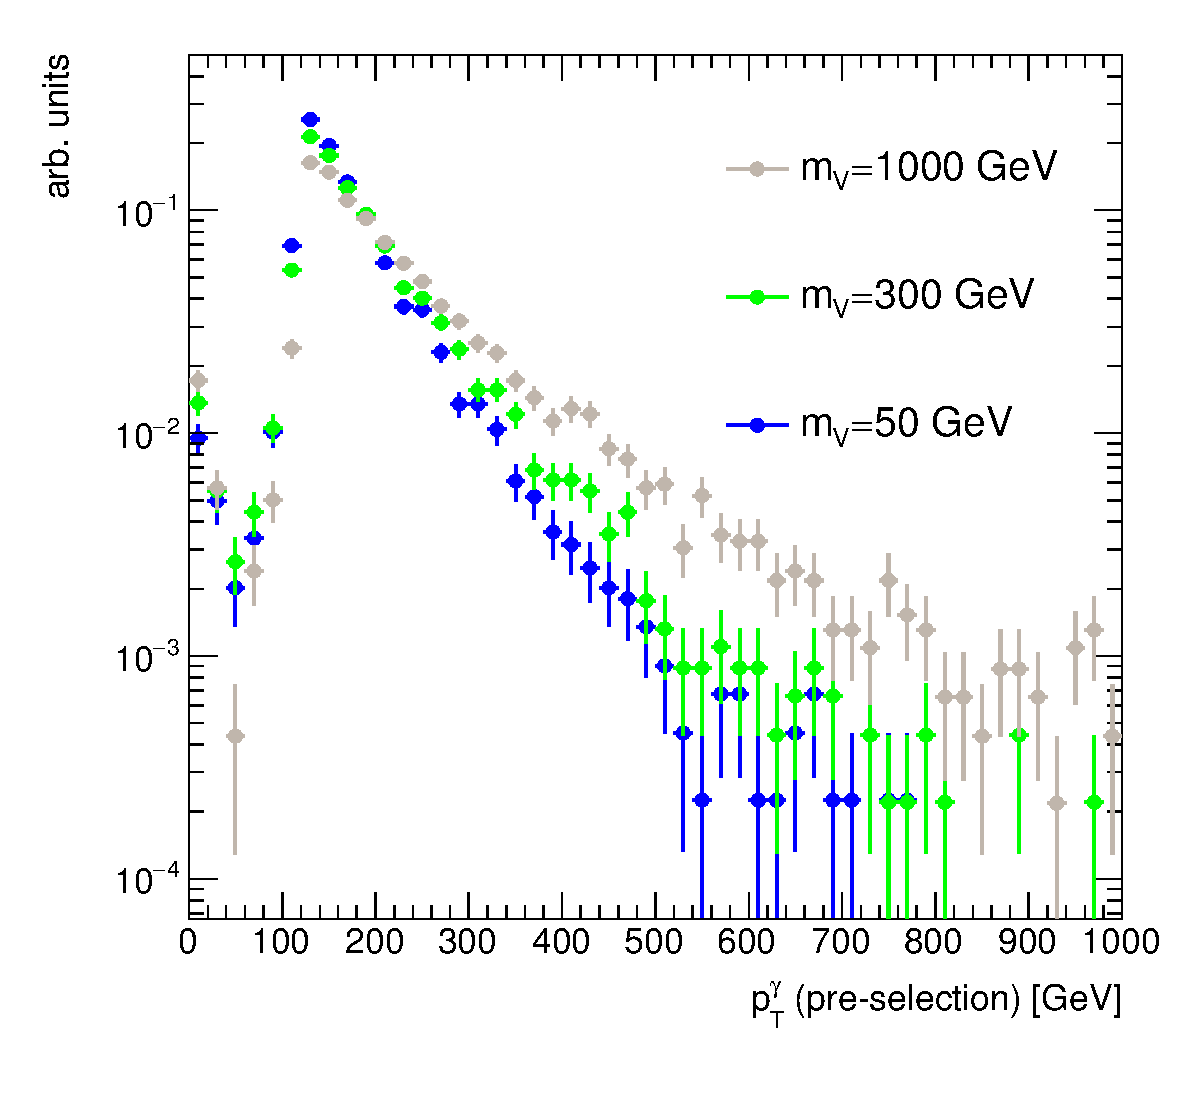
\includegraphics[width=0.45\textwidth]{figures/EW/ptGamma_filter120GeV_dmV_dm10GeV}
}%TODO: add this + equivalent plot of \MET to appendix
\hfill
\subfloat[Leading photon transverse momentum distribution for the photon+\MET final state, 
for different DM mass choices, with \mMed=1~\tev.\label{fig:DMV_EW_gamma_pT_SVMed}]{%
		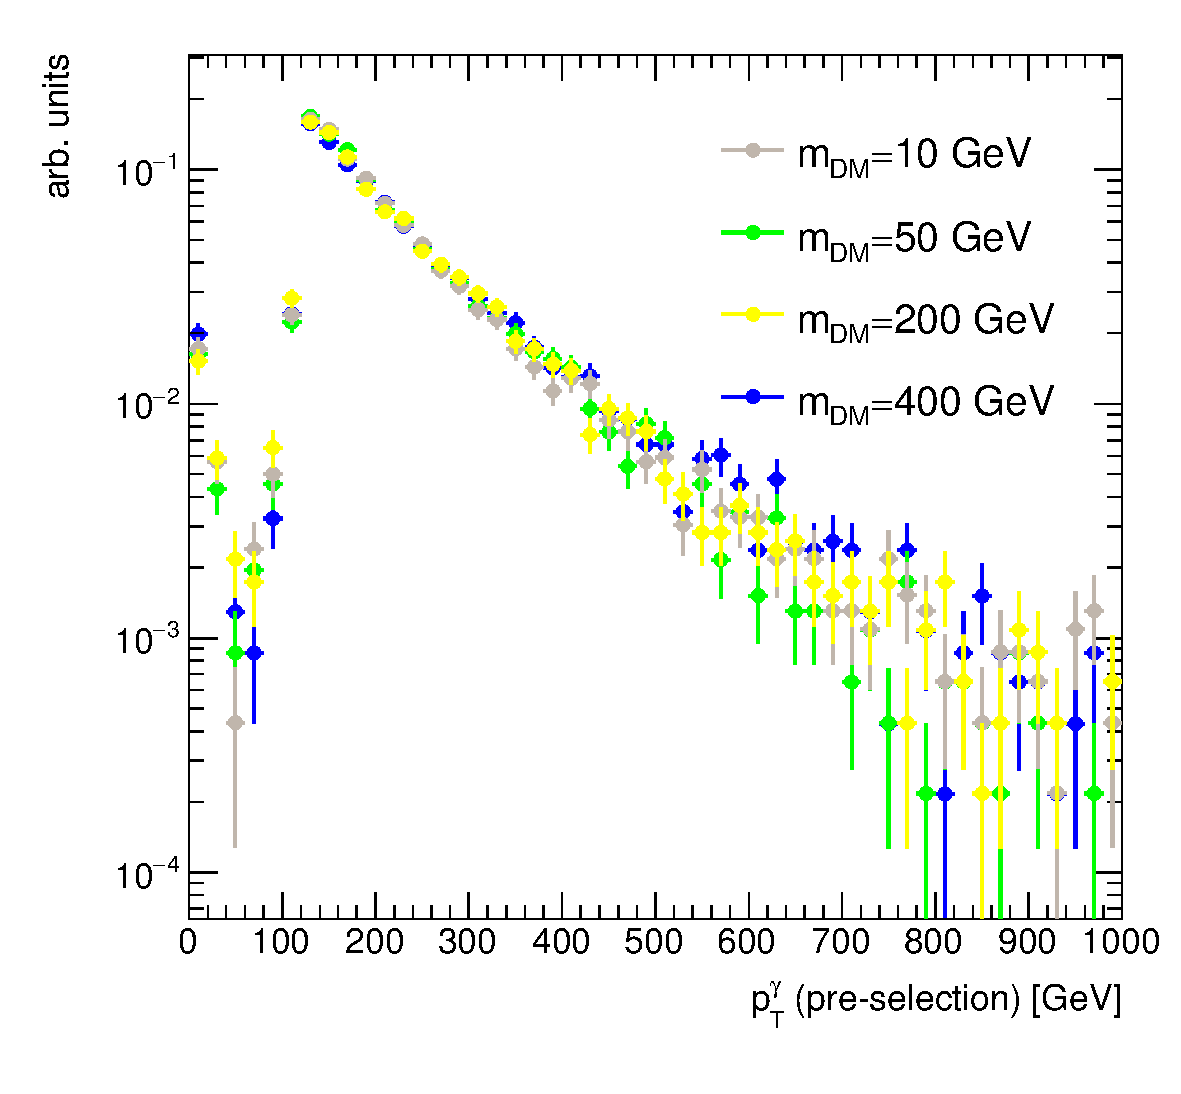
\includegraphics[width=0.45\textwidth]{figures/EW/ptGamma_filter120GeV_dmV_mV1000GeV}
}%TODO: add equivalent plot of \MET to appendix
\hfill
\subfloat[Missing transverse momentum distribution for the leptonic Z+\MET final state, 
for different mediator mass choices, for \mdm=15~\gev\label{fig:DMV_EW_Z_MET_SVMed}]{%
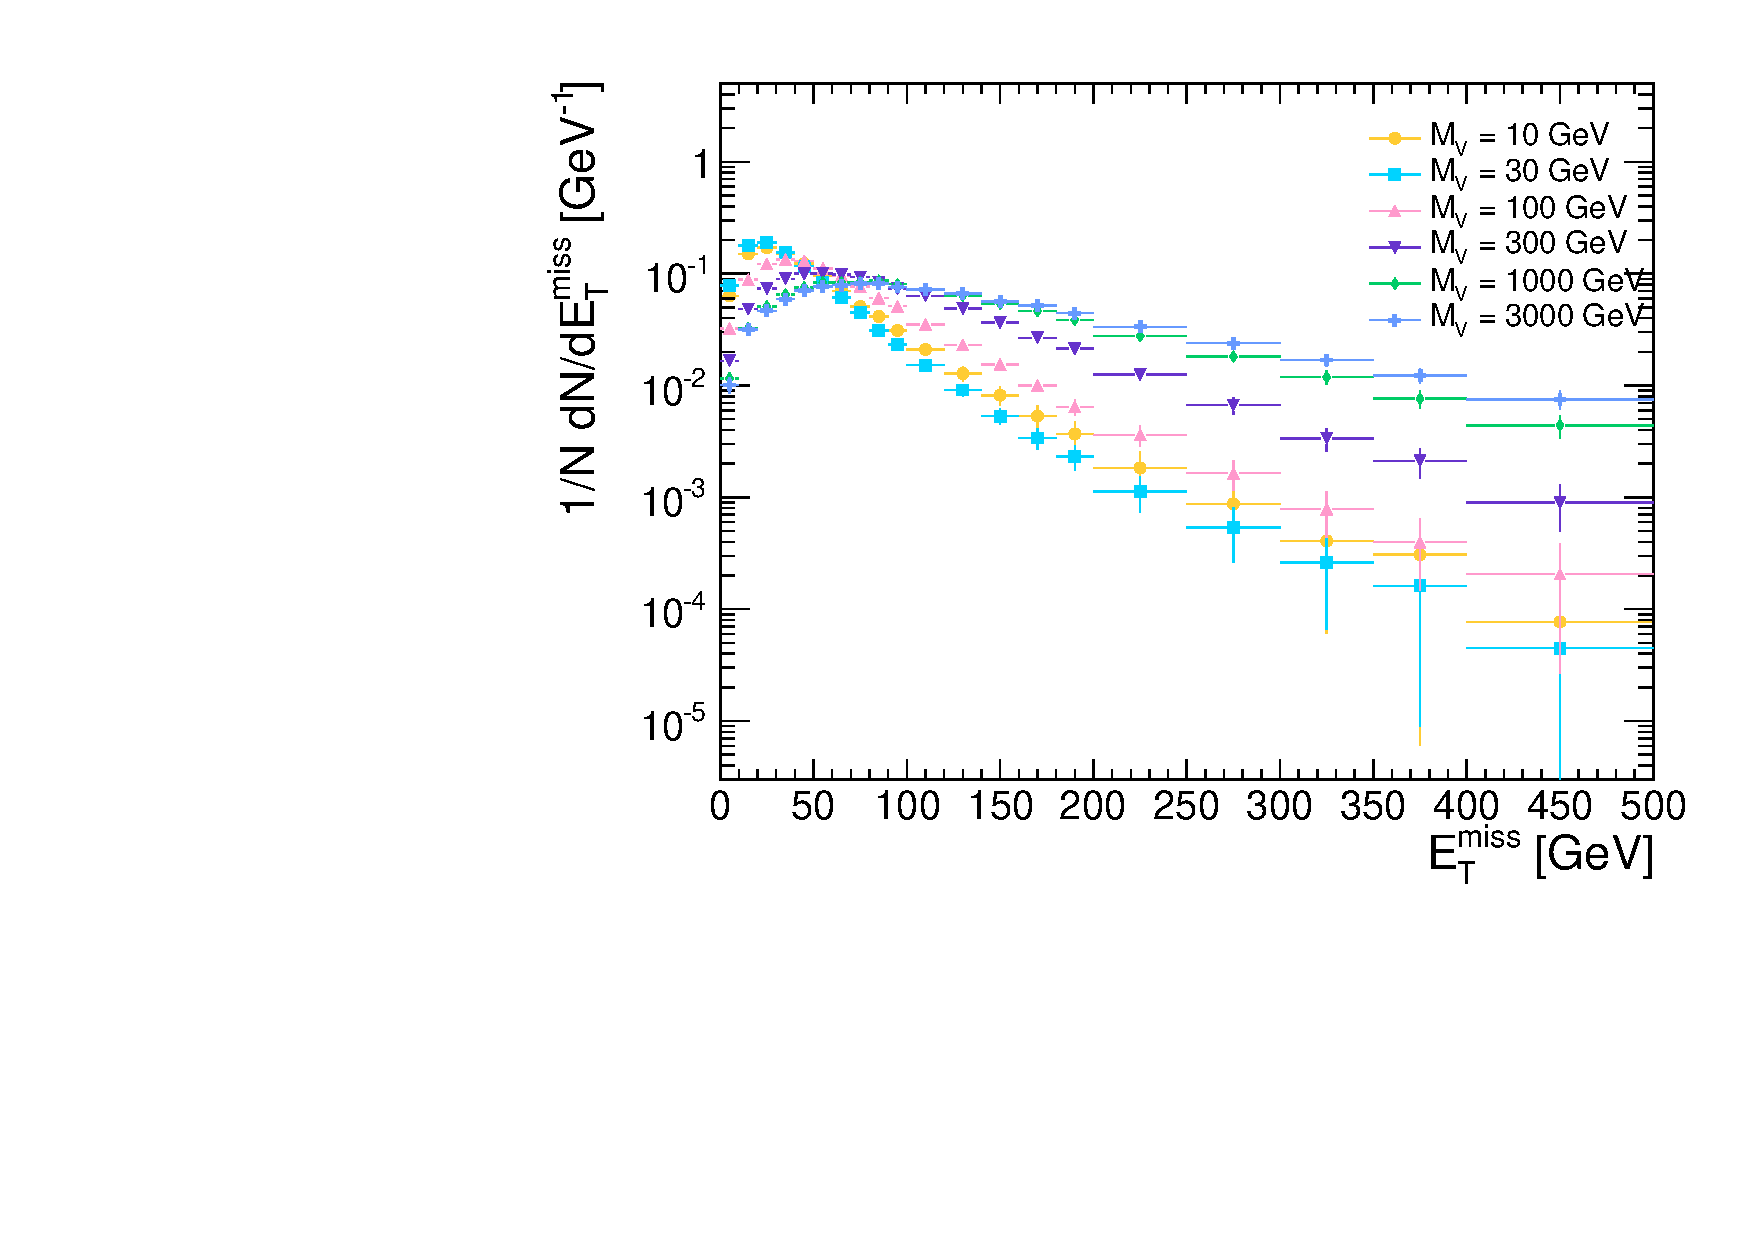
\includegraphics[width=0.45\textwidth]{figures/EW/pt_vv_Mx15}
}    
\hfill
\subfloat[Missing transverse momentum distribution for the hadronic W+\MET final state.\label{fig:DMV_EW_Whad_MET_SVMed}]{%
	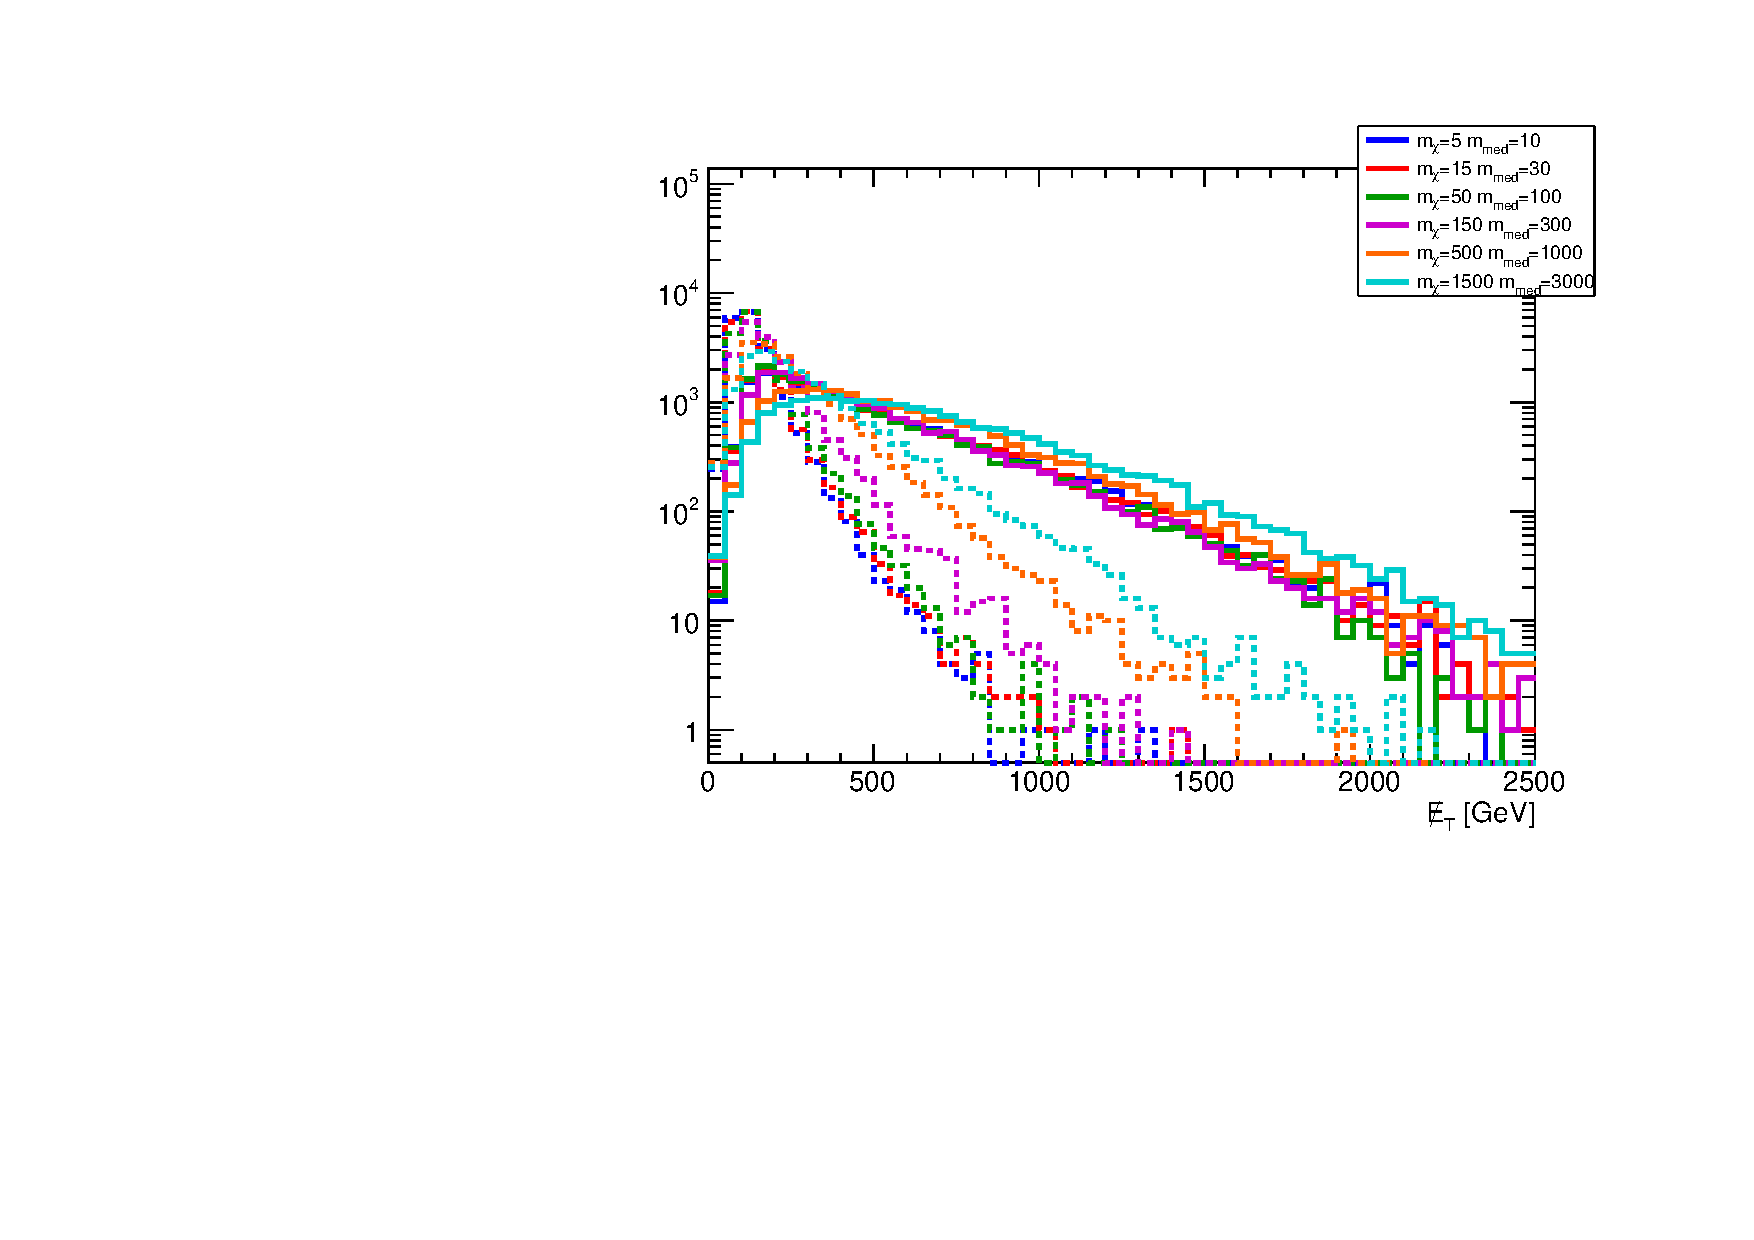
\includegraphics[width=0.5\textwidth]{figures/EW/monoWhad_Destructive/metPt}
}    
\caption{Kinematic distributions relevant for searches with W, Z and photons in the final state, 
for the simplified model
       with a vector mediator exchanged in the $s-$channel.}
\label{fig:DMV_EW_kinematics_SVMed}
\end{figure}


%%%%%%%%%%%%%%%
%%%%%%%%%%%%%%%
%%%%%%%%%%%%%%%
% S/P SIMPLIFIED MODELS%
%%%%%%%%%%%%%%%
%%%%%%%%%%%%%%%
%%%%%%%%%%%%%%%

\section{Scalar and pseudoscalar mediator, \schannel exchange}
\label{sec:monojet_scalar}

\begin{figure}
\centering
\unitlength=0.005\linewidth
	\subfloat[\label{subfig:appendixmodelSmonojetTopTriangle}]	{
	\begin{feynmandiagram}[appendixmodelSmonojetTopTriangle]
		\fmfleft{i1,i2}
		\fmfright{o1,o2}
		\fmftop{isr}
		\fmfbottom{pisr}
		\fmfpolyn{empty}{v}{3}
		\fmf{fermion}{i2,v6}
		\fmf{phantom}{i1,pv1,v1}
		\fmf{gluon,tension=0}{i1,v1}
		\fmf{gluon}{v6,v3}
		\fmf{dashes,label={\LARGE $S,,P$}}{v2,v5}
		\fmf{fermion,tension=1.2}{o2,v5,o1}
		\fmfdot{v1,v6,v2,v3,v5}
		\fmffreeze
		\fmf{phantom}{pv1,pisr}
		\fmf{fermion}{v6,isr}
		\fmflabel{\LARGE ${g}$}{i1}
		\fmflabel{\LARGE ${q}$}{i2}
		\fmflabel{\LARGE ${q}$}{isr}
		\fmflabel{\LARGE $\bar\chi$}{o1}
		\fmflabel{\LARGE $\chi$}{o2}
	\end{feynmandiagram}
}
	\subfloat[\label{subfig:appendixmodelSmonojetTopBox}]	{
	\begin{feynmandiagram}[appendixmodelSmonojetTopBox]
		\fmfleft{i1,i2}
		\fmfright{o1,o2,hisr,isr}
		\fmfpolyn{empty}{v}{4}
		\fmf{gluon}{i2,v4}
		\fmf{gluon}{i1,v1}
		\fmf{dashes,label={\LARGE $S,,P$}}{v2,vwimp}
		\fmflabel{\LARGE ${g}$}{i1}
		\fmflabel{\LARGE ${g}$}{i2}
		\fmflabel{\LARGE ${g}$}{isr}
		\fmflabel{\LARGE $\bar\chi$}{o1}
		\fmflabel{\LARGE $\chi$}{o2}
		\fmf{fermion}{o2,vwimp,o1}
		\fmfdot{v1,v2,v3,v4,vwimp}
		\fmf{gluon}{v3,isr}
	\end{feynmandiagram}
}
\setfloatalignment{t}
\vspace{0.5\baselineskip}
	\caption
	{
		One-loop diagrams of processes exchanging a scalar ($S$) or pseudoscalar ($P$) mediator, leading to a mono-jet signature. 
	}
	\label{fig:feyn_prod_S}
\end{figure}

In this section, we consider a parallel situation to the vector and axial-vector mediators in the previous sections: a real scalar or a pseudoscalar where the associated scalar is decoupled at higher energies\sidenote{This assumption does not hold in a UV-complete model where the two components of the complex scalar mediator would be approximately degenerate.  The complex scalar case could be studied separately in the case of heavy flavor final states given the sufficiently different kinematics.}. This section is largely based on Refs.~\cite{Buckley:2014fba,Harris:2014hga} which contain a thorough discussion of these models. 

Assuming MFV, \spinzero resonances behave in a similar fashion as the SM Higgs boson. Relative to the vector and axial-vector models discussed above, the scalar models are distinguished by the special consequences of the MFV assumption: the very narrow width of the mediator and its extreme sensitivity to which decays are kinematically available, and the loop-induced coupling to gluons. The interaction Lagrangians are

\begin{fullwidth}
  \begin{eqnarray} {\cal L}_{\phi} & = &
    % {\cal L}_{\rm SM}+i\bar{\chiDM} \slashed{\partial} \chiDM + \mDM \bar{\chiDM}\chiDM + \left| \partial_\mu \phi \right|^2+\frac{1}{2}m_\phi^2 \phi^2 + \nonumber \\
    % & &
          \gdm \phi \bar{\chiDM}\chiDM+ \frac{\phi}{\sqrt{2}} \sum_i \left(g_u y_i^u \bar{u}_i u_i+g_d y_i^d \bar{d}_i d_i+g_\ell y_i^\ell \bar{\ell}_i \ell_i\right)\, , \label{eq:scalarlag} \\
    {\cal L}_{a} & = &
    % {\cal L}_{\rm SM}+i\bar{\chiDM} \slashed{\partial} \chiDM + \mDM \bar{\chiDM}\chiDM + \left| \partial_\mu a \right|^2+\frac{1}{2}m_a^2 a^2 + \nonumber \\
    % & &
          i\gdm a \bar{\chiDM}\gamma_5\chiDM+ \frac{i a}{\sqrt{2}}\sum_i  \left(g_u y_i^u \bar{u}_i \gamma_5 u_i+g_d y_i^d \bar{d}_i \gamma_5 d_i+ \right. \nonumber \\
                                   & & \left. g_\ell y_i^\ell   \bar{\ell}_i \gamma_5 \ell_i\right) \,. \label{eq:pseudoscalarlag}
  \end{eqnarray}
\end{fullwidth}
where $\phi$ and $a$ are respectively the scalar and pseudoscalar mediators, and the Yukawa couplings $y_i^f$ are normalized to the Higgs vev as $y_i^f = \sqrt{2}m_i^f/v$.

The couplings to fermions are proportional to the SM Higgs couplings, yet one is still allowed to adjust an overall strength of the coupling to charged leptons and the relative couplings of $u$- and $d$-type quarks. As in the preceding sections, for the sake of simplicity and straightforward comparison, we reduce the couplings to the SM fermions to a single universal parameter $\gq \equiv g_u = g_d = g_\ell$. Unlike the vector and axial-vector models, the scalar mediators are allowed to couple to leptons.\sidenote{This contribution plays no role for most of the parameter space considered. The choice to allow lepton couplings follows Refs.~\cite{Buckley:2014fba,Harris:2014hga}.}


The relative discovery and exclusion power of each search can be compared in this framework.
However, we again emphasize the importance of searching the
full set of allowed channels in case violations of these simplifying assumptions
lead to significant modifications of the decay rates that
unexpectedly favor different
channels than the mix obtained under our assumptions. The coupling $\gdm$ parameterizes the entire dependence on the structure between the mediator and the dark sector.

%The most general Lagrangians including new scalars or pseudoscalars will have a potential containing interactions with the SM Higgs field $h$. 
 %If there is no indication otherwise the easiest assumptions is always the most scientific to chose (also listening to some phenomenologists this seems not always to be the case ;-) )  

Given these simplifications, the minimal set of parameters under consideration is
 \bea
  \left\{ \mDM,~ m_{\phi/a} = \mMed,~ \gdm,~ \gq \right\} \,.
 \eea
Fig.~\ref{fig:feyn_prod_S} shows the one-loop diagrams producing a jet+X signature. 
The full calculation of the top loop is available at LO for DM pair production in association 
with one parton. 


%The simplest choice of couplings, known as Minimal Simplified Dark Matter model (MSDM) \textbf{[TODO: add references]}, is $g_u = g_d = g_\ell$, which is realized in singlet scalar extensions of the SM. 

% Despite our simplifying assumption, one should keep the more general possibility in mind, as even simple extensions of the mediating sector can result in $g_u \neq g_d \neq g_\ell$. A well-known realization of this would be the coupling of the pseudoscalar to up-type quarks (proportional to $m_u \cot\beta$) and down-type quarks and charged leptons (proportional to $m_{d/\ell}\tan\beta$) in two-Higgs doublet extensions of the SM. Here $\tan \beta$ denoting the ratio of vacuum expectation values of the two Higgs doublets. %The case $g_u \neq  g_d \neq g_\ell$ requires additional scalars with potentially large masses. 
% This possibility of non-equal couplings motivates searches in complementary channels which probe couplings to different flavors of quarks and leptons.

%Extending the SM Higgs sector to a two Higgs doublet model implies more complex couplings such as  $g_u = \cot \beta$ and $g_d = g_e = \tan \beta$ where $\tan \beta$ denotes the ratio of vacuum expectation values of the two Higgs doublets.  The case $g_u \neq  g_d \neq g_\ell$ requires more additional scalars with potentially large masses, and it is not covered here: for simplicity, we assume universal SM-mediator couplings $g_v = g_u = g_d = g_\ell$ in the remainder of this work. 


%The model assumes Dirac Dark Matter particles and is based on the minimal flavor violation (MFV), which motivates Higgs-like Yukawa couplings of the mediator to the Standard Model quarks. No other couplings, such as to leptons, are allowed in this model.
%The following two cases are considered:\\
%(a) scalar couplings to DM and SM,\\
%(b) pseudo-scalar couplings to DM and SM\\
%\noindent with the corresponding Lagrangians written as:
%\begin{align}
%\label{eq:SP} 
%\mathcal{L}_{\mathrm{scalar}} &= \gq \sum \frac{m_q}{v} (\bar{q}q) S + \gDM (\bar{\chiDM}\chiDM) S \\
%\mathcal{L}_{\mathrm{pseudo-scalar}} &= \gq \sum \frac{m_q}{v} (\bar{q}\gamma^5q) P + \gDM (\bar{\chiDM}\gamma^5\chiDM) P \\
%\end{align}
%where $v=246$~\gev denotes the Higgs vacuum expectation value.

The minimal mediator width is given by %Eq.\,\ref{eq:monojet_min},
\begin{fullwidth}
  \begin{equation} \label{eq:width}
    \begin{split}
      \Gamma_{\phi,a} = & \sum_f N_c \frac{y_f^2 \gq^2 m_{\phi,a}}{16
        \pi} \left(1-\frac{4 m_f^2}{m_{\phi,a}^2}\right)^{x/2}
      + \frac{\gdm^2 m_{\phi,a}}{8 \pi} \left(1-\frac{4 \mDM^2}{m_{\phi,a}^2}\right)^{x/2}\\
      & + \frac{\alpha_s^2 y_t^2 \gq^2 m_{\phi,a}^3}{32 \pi^3 v^2}
      \left| f_{\phi,a}\left(\tfrac{4m_t^2}{m_{\phi,a}^2}
        \right)\right|^2
    \end{split}
  \end{equation}
\end{fullwidth}
where $x=3$ for scalars and $x=1$ for pseudoscalars. The loop integrals are
\begin{fullwidth}
  \bea \label{eq:fphifa}
  f_\phi (\tau) &=& \tau \left [ 1+ (1-\tau) \arctan^2 \left ( \frac{1}{\sqrt{\tau-1}} \right ) \right ]  \,, \\
  f_a (\tau) &=& \tau \arctan^2 \left ( \frac{1}{\sqrt{\tau-1}}
  \right) \, 
  \eea
\end{fullwidth}
for mediator masses above the top threshold, $\tau > 1$, where $\tau = 4 m_{t}^2/m_{\phi,a}^2$, and, for mediator masses below the top threshold, $\tau < 1$, 
\begin{fullwidth}
  \bea \label{eq:fphifb}
  f_\phi (\tau) &=& \tau \left [ 1+ (1-\tau)\left(-\frac{1}{4}\left(\log\frac{1+\sqrt{1-\tau}}{1-\sqrt{1-\tau}}+i\pi\right)^2\right) \right ]  \,\,,\\
  f_a (\tau) &=& \tau
  \left(-\frac{1}{4}\left(\log\frac{1+\sqrt{1-\tau}}{1-\sqrt{1-\tau}}+i\pi\right)^2\right).
  \eea
\end{fullwidth}


% If this is in the DM@LHC write-up, it is unnecessary here.
% The first term in the width corresponds to the decay into SM fermions, and the sum runs over all kinematically available fermions, $N_c = 3$ for quarks. The second term is the decay into DM, assuming that is kinematically allowed. The factor of two between the decay into SM  fermions and into DM  is a result of our choice of normalization of the Yukawa couplings due to spin dependencies. The last term corresponds to decay into gluons.  Since we have assumed that $\gq = g_u = g_d = g_\ell$, we have included in the partial decay widths $\Gamma (\phi/a \to gg)$ only the contributions stemming from top loops, which provide the by far largest corrections given that $y_t \gg y_b$~etc. At the loop level the mediators can decay not only to gluons but also to pairs of photons and other final states if kinematical accessible. However the decay rates $\Gamma (\phi/a \to gg)$ are always larger than the other loop-induced partial widths, and in consequence the total decay widths $\Gamma_{\phi/a}$ are well approximated by the corresponding sum of the individual partial decay widths involving DM, fermion or gluon pairs. It should be noted that if  $m_{\phi/a} > 2m_t$ the total widths of $\phi/a$ will typically be dominated by the partial widths to top quarks.


%\begin{equation}
%\Gamma_{\rm{min}}^{S/P}=\Gamma_{\bar{\chiDM}\chiDM}^{S/P} + \sum_{q}\Gamma_{\bar{q}q}^{S/P} + \Gamma_{gg}^{S/P},
%\end{equation}
%with the following LO expressions for the partial widths:
%\begin{align}
%\Gamma_{\bar{\chiDM}\chiDM}^{\rm{S}}&=\frac{\gDM^2 \mMed}{8\pi}\beta_{DM}^{3/2} \theta(\mMed-2\mDM)\\
%\Gamma_{\bar{q}q}^{\rm{S}}&= \frac{3 \gq^2 \mMed}{8\pi}\frac{m_q^2}{v^2}\beta_q^{3/2} \theta(\mMed-2m_q)\\
%\Gamma_{gg}^{\rm{S}}&= \frac{\gq^2 \alpha_s^2}{2\pi^3 v^2 \mMed} \left| \sum_q m_q^2 F_{\rm{S}} \left( \frac{4m_q^2}{\mMed^2} \right) \right|^2\\
%\Gamma_{\bar{\chiDM}\chiDM}^{\rm{P}}&=\frac{\gDM^2 \mMed}{8\pi} \beta_{DM}\theta(\mMed-2\mDM)\\
%\Gamma_{\bar{q}q}^{\rm{P}}&= \frac{3 \gq^2 \mMed}{8\pi}\frac{m_q^2}{v^2}\beta_{q}\theta(\mMed-2m_q)\\
%\Gamma_{gg}^{\rm{P}}&= \frac{\gq^2 \alpha_s^2}{2\pi^3 v^2 \mMed} \left| \sum_q m_q^2 F_{\rm{P}} \left( \frac{4m_q^2}{\mMed^2} \right) \right|^2\;,
%\label{eq:GammaS}
%\end{align}
%with the form factors defined as
%\begin{align}
%F_{\rm{S}}(x)&= 1+(1-x)\arctan^2\left(\frac{1}{\sqrt{x-1}}\right)\\
%F_{\rm{P}}(x)&= \arctan^2\left(\frac{1}{\sqrt{x-1}}\right)\;.
%\end{align}

%%Start Matt Buckley's edits 
%\begin{equation} \label{eq:width}
%\begin{split}
%\Gamma_{\phi,a}  = & \sum_f N_c \frac{y_f^2 \gq^2 m_{\phi,a}}{16 \pi} \left(1-\frac{4 m_f^2}{m_{\phi,a}^2}\right)^{x/2}
%+ \frac{\gdm^2 m_{\phi,a}}{8 \pi} \left(1-\frac{4 \mDM^2}{m_{\phi,a}^2}\right)^{x/2}\\
%& + \frac{\alpha_s^2 y_t^2 \gq^2 m_{\phi,a}^3}{32 \pi^3 v^2} \left| f_{\phi,a}\left(\tfrac{4m_t^2}{m_{\phi,a}^2} \right)\right|^2
%\end{split}
%\end{equation}
%
%where $x=3$ for scalars and $x=1$ for pseudoscalars, and the loop integrals are
%
%\bea \label{eq:fphifa}
%f_\phi (\tau) = \tau \left [ 1+ (1-\tau) \arctan^2 \left ( \frac{1}{\sqrt{\tau-1}} \right ) \right ]  \,, \qquad 
%f_a (\tau) =  \tau \arctan^2 \left ( \frac{1}{\sqrt{\tau-1}} \right ) \,. 
%\eea
%
%The first term in each width corresponds to the decay into SM fermions (the sum runs over all kinematically available fermions, $N_c = 3$ for quarks and $N_c = 1$ for leptons). The second term is the decay into DM (assuming that this decay is kinematically allowed). The factor of two between the decay into SM  fermions and into DM  is a result of our choice of normalization of the Higgs vacuum expectation value and the Yukawa couplings.
%

%%BP: Is this the best way to express that? I'd add:... due to spin dependencies. 
%%MB: yes. I don't think it's a spin thing, it's just that we've defined v = 246, so the SM fermions get a $1/\sqrt{2}^2$ that DM doesn't.

%The last two terms correspond to decay into gluons.  Since we have assumed that $\gq = g_u = g_d = g_\ell$, we have included in the partial decay widths $\Gamma (\phi/a \to gg)$ only the contributions stemming from top loops, which provide the by far largest corrections given that $y_t \gg y_b$~etc. At the loop level the mediators can decay not only to gluons but also to pairs of photons and other final states if kinematical accessible. However the decay rates $\Gamma (\phi/a \to gg)$ are always larger than the other loop-induced partial widths, and in consequence the total decay widths $\Gamma_{\phi/a}$ are well approximated by the corresponding sum of the individual partial decay widths involving DM, fermion or gluon pairs. It should be noted that if  $m_{\phi/a} > 2m_t$ the total widths of $\phi/a$ will typically be dominated by the partial widths to top quarks.

%%%End Matt Buckley's edits

The minimal widths for scalar and pseudo-scalar mediators with $\gq=\gDM=1$ are shown in Fig.\,\ref{fig:monojet_width_S}, illustrating the effect of choosing
the SM Higgs-like Yukawa couplings for the SM fermions.
For the mediator mass above twice the top quark mass $m_t$, the minimal width receives the dominant contribution from the top quark. For lighter mediator masses, Dark Matter dominates as the couplings to lighter quarks are Yukawa suppressed.
%Note that the partial width coming from gluons through loops can be safely neglected\,\cite{Haisch:2015ioa}.

As shown in the diagram of Fig.~\ref{fig:feyn_prod_S}, the lowest order process of these models
already involves a one-loop amplitude in QCD, and only LO predictions are currently available. 
The generator used for the studies in this Section is \powheg~\cite{Haisch:2015ioa}; within this implementation,
the scalar and pseudoscalar mediator benchmark models are known at LO+PS accuracy. 

\subsection{Parameter scan}

Similarly as in the case of the vector and axial-vector couplings
of \spinone mediators, scans in the parameter space are performed also for the scalar and pseudo-scalar couplings of the \spinzero mediators
in order to decide on the optimized parameter grid for the presentation of Run-2 results. Figures\,\ref{fig:monojet_scan_S_g}-
%, fig:monojet_scan_S_mDM1000,fig:monojet_scan_S_mDM100, fig:monojet_scan_S_mMed10, 
\ref{fig:monojet_scan_S_mMed1000} show the scans over the couplings, Dark Matter mass and mediator mass and the same conclusions apply as in Section\,\ref{sec:monojet_V}.

A scan over the mediator mass is shown in Fig.\,\ref{fig:monojet_scan_S_mMed1000} where \mMed = 300~\gev and 500~\gev are chosen to be below and above $2m_t$. The off-shell Dark Matter production regime is assumed by taking an extreme limit ($\mDM=1$~\tev) in order to study solely the effects of the couplings to quarks. 
No differences in the kinematic distributions are observed and also the cross sections remain similar in this case. No significant changes appear for mediator masses around the $2m_t$ threshold.

\begin{figure*}[!htpb]
\centering
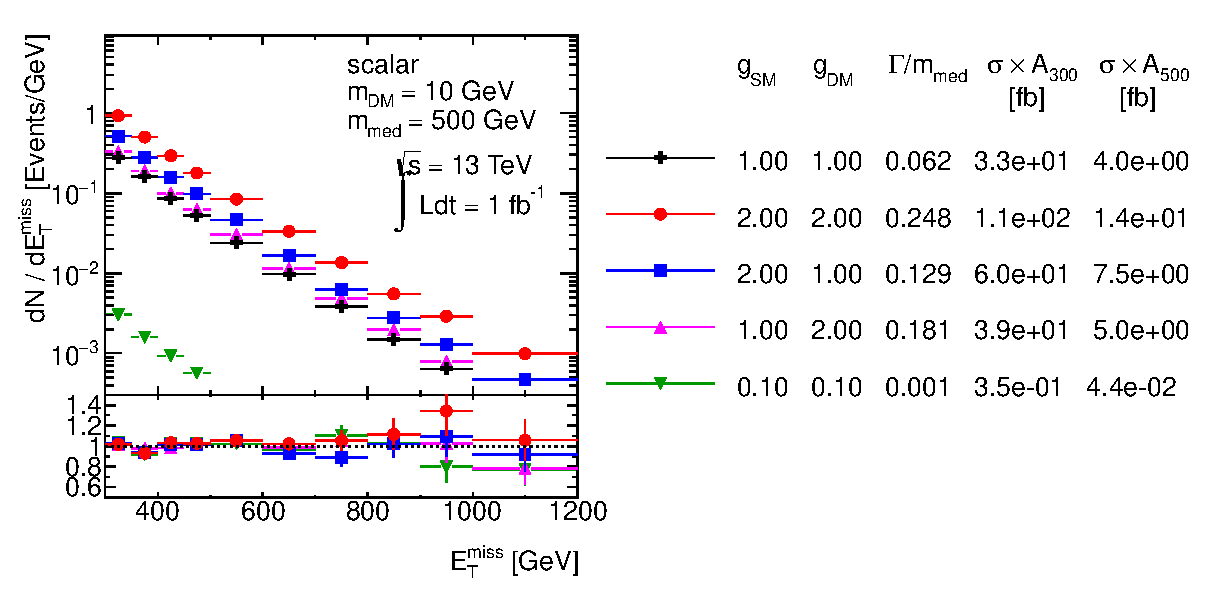
\includegraphics[width=0.95\textwidth]{figures/monojet/scan_g_S_10_500.eps}
\caption{Scan over couplings. The $\MET$ distribution is compared for the scalar mediator models using the parameters as indicated. Ratios of the normalized distributions with respect to the first one are shown. $A_{300}$ and $A_{500}$ in the table denote the acceptance of the $\MET>300$~\gev and $\MET>500$~\gev cut, respectively.}
\label{fig:monojet_scan_S_g}
\end{figure*}

\begin{figure*}[!htpb]
\centering
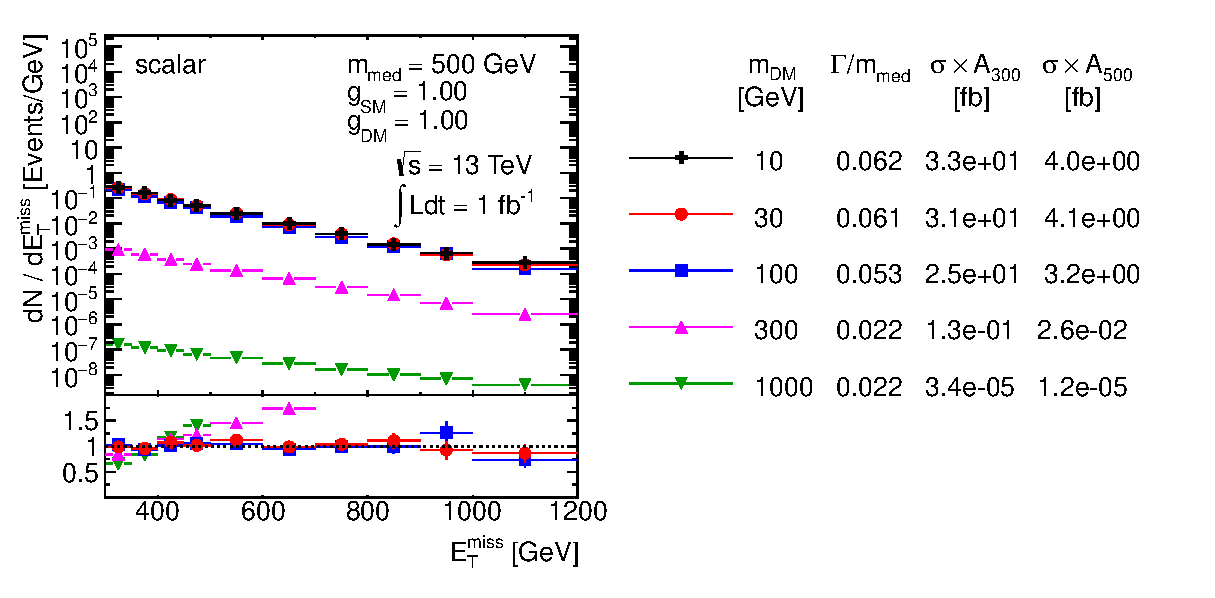
\includegraphics[width=0.95\textwidth]{figures/monojet/scan_mDM_S_500.eps}
\caption{Scan over Dark Matter mass. The $\MET$ distribution is compared for the scalar mediator models using the parameters as indicated. Ratios of the normalized distributions with respect to the first one are shown. $A_{300}$ and $A_{500}$ in the table denote the acceptance of the $\MET>300$~\gev and $\MET>500$~\gev cut, respectively.}
\label{fig:monojet_scan_S_mDM1000}
\end{figure*}

\begin{figure*}[!htpb]
\centering
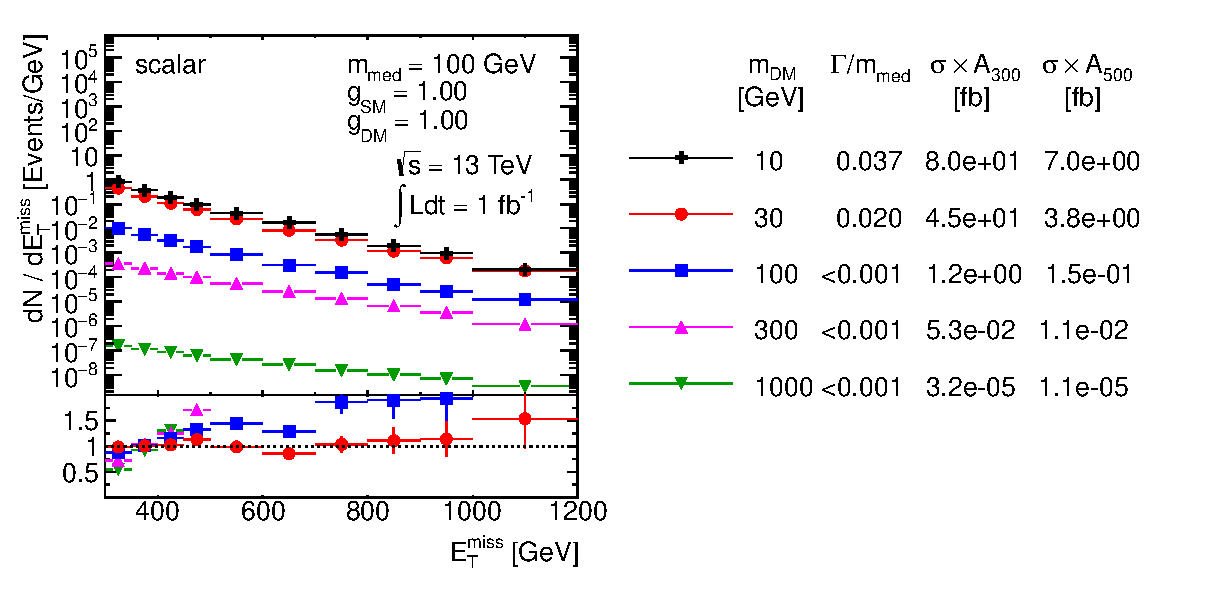
\includegraphics[width=0.95\textwidth]{figures/monojet/scan_mDM_S_100.eps}
\caption{Scan over Dark Matter mass. The $\MET$ distribution is compared for the scalar mediator models using the parameters as indicated. Ratios of the normalized distributions with respect to the first one are shown. $A_{300}$ and $A_{500}$ in the table denote the acceptance of the $\MET>300$~\gev and $\MET>500$~\gev cut, respectively.}
\label{fig:monojet_scan_S_mDM100}
\end{figure*}

\begin{figure*}[!htpb]
\centering
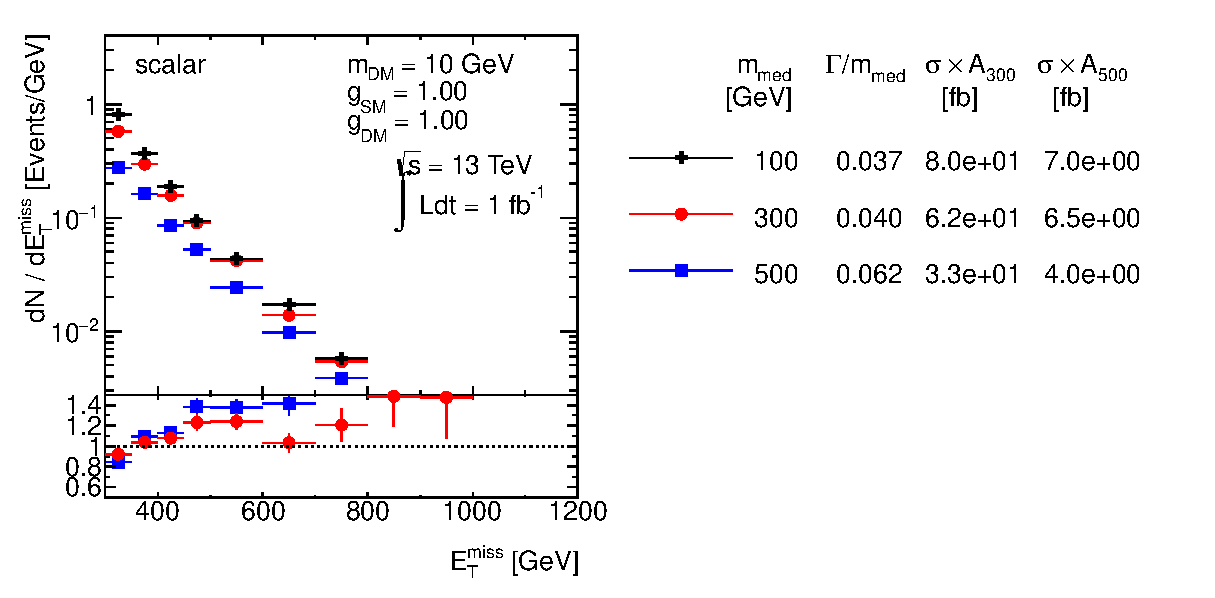
\includegraphics[width=0.95\textwidth]{figures/monojet/scan_mMed_S_10.eps}
\caption{Scan over mediator mass. The $\MET$ distribution is compared for the scalar mediator models using the parameters as indicated. Ratios of the normalized distributions with respect to the first one are shown. $A_{300}$ and $A_{500}$ in the table denote the acceptance of the $\MET>300$~\gev and $\MET>500$~\gev cut, respectively.}
\label{fig:monojet_scan_S_mMed10}
\end{figure*}

\begin{figure*}[!htpb]
\centering
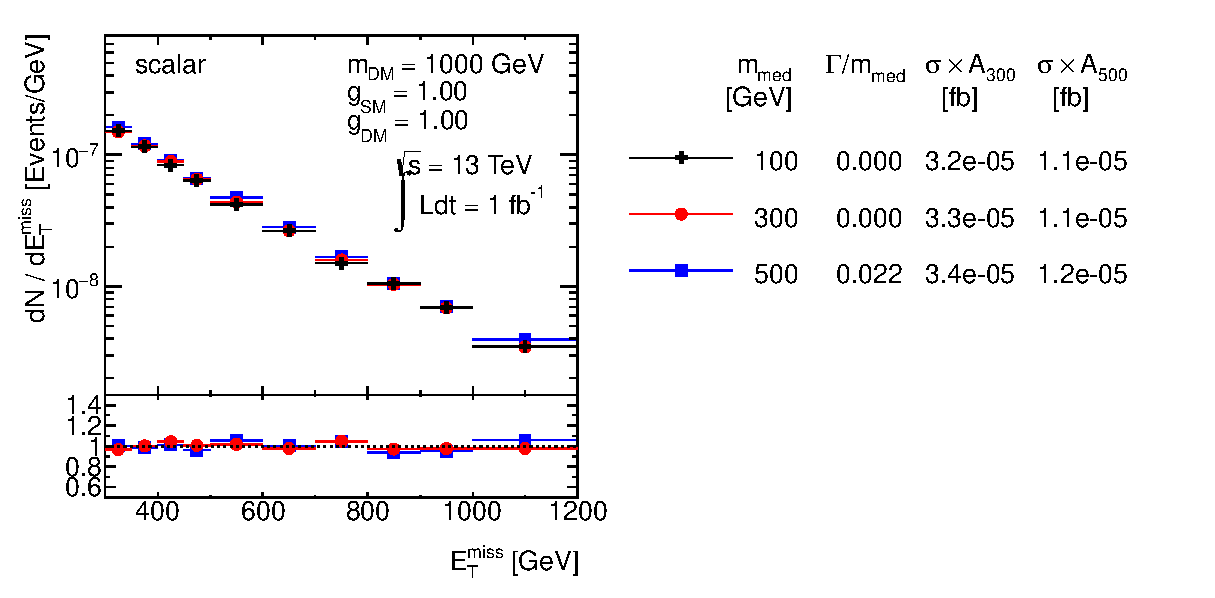
\includegraphics[width=0.95\textwidth]{figures/monojet/scan_mMed_S_1000.eps}
\caption{Scan over mediator mass. The $\MET$ distribution is compared for the scalar mediator models using the parameters as indicated. Ratios of the normalized distributions with respect to the first one are shown. $A_{300}$ and $A_{500}$ in the table denote the acceptance of the $\MET>300$~\gev and $\MET>500$~\gev cut, respectively.}
\label{fig:monojet_scan_S_mMed1000}
\end{figure*}

\begin{figure}
	\centering
	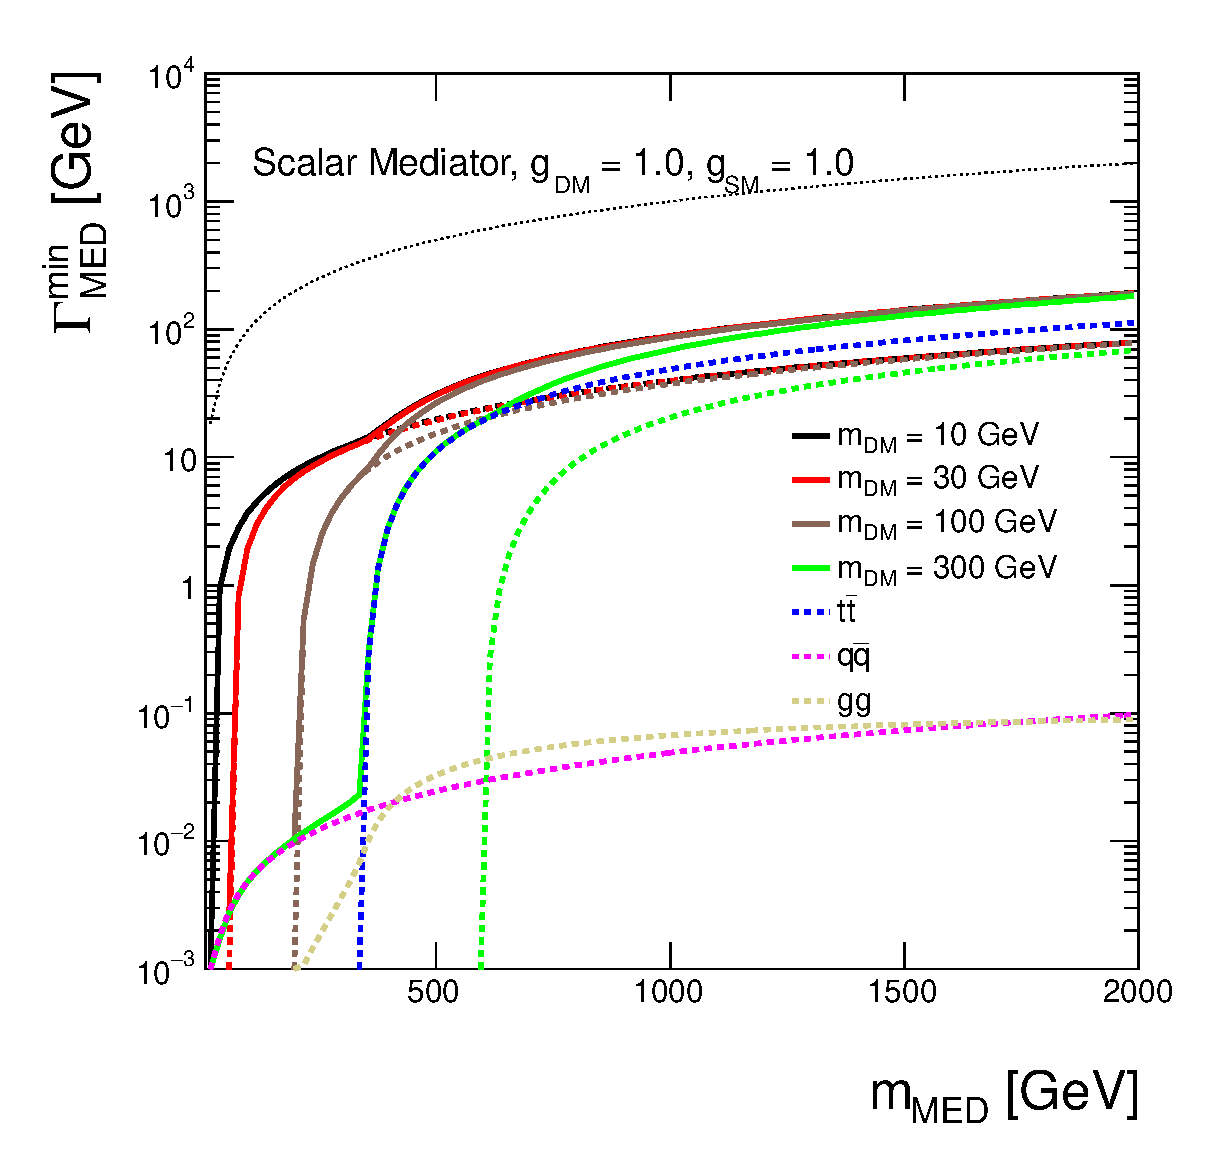
\includegraphics[width=0.95\textwidth]{figures/monojet/width_S.eps}
	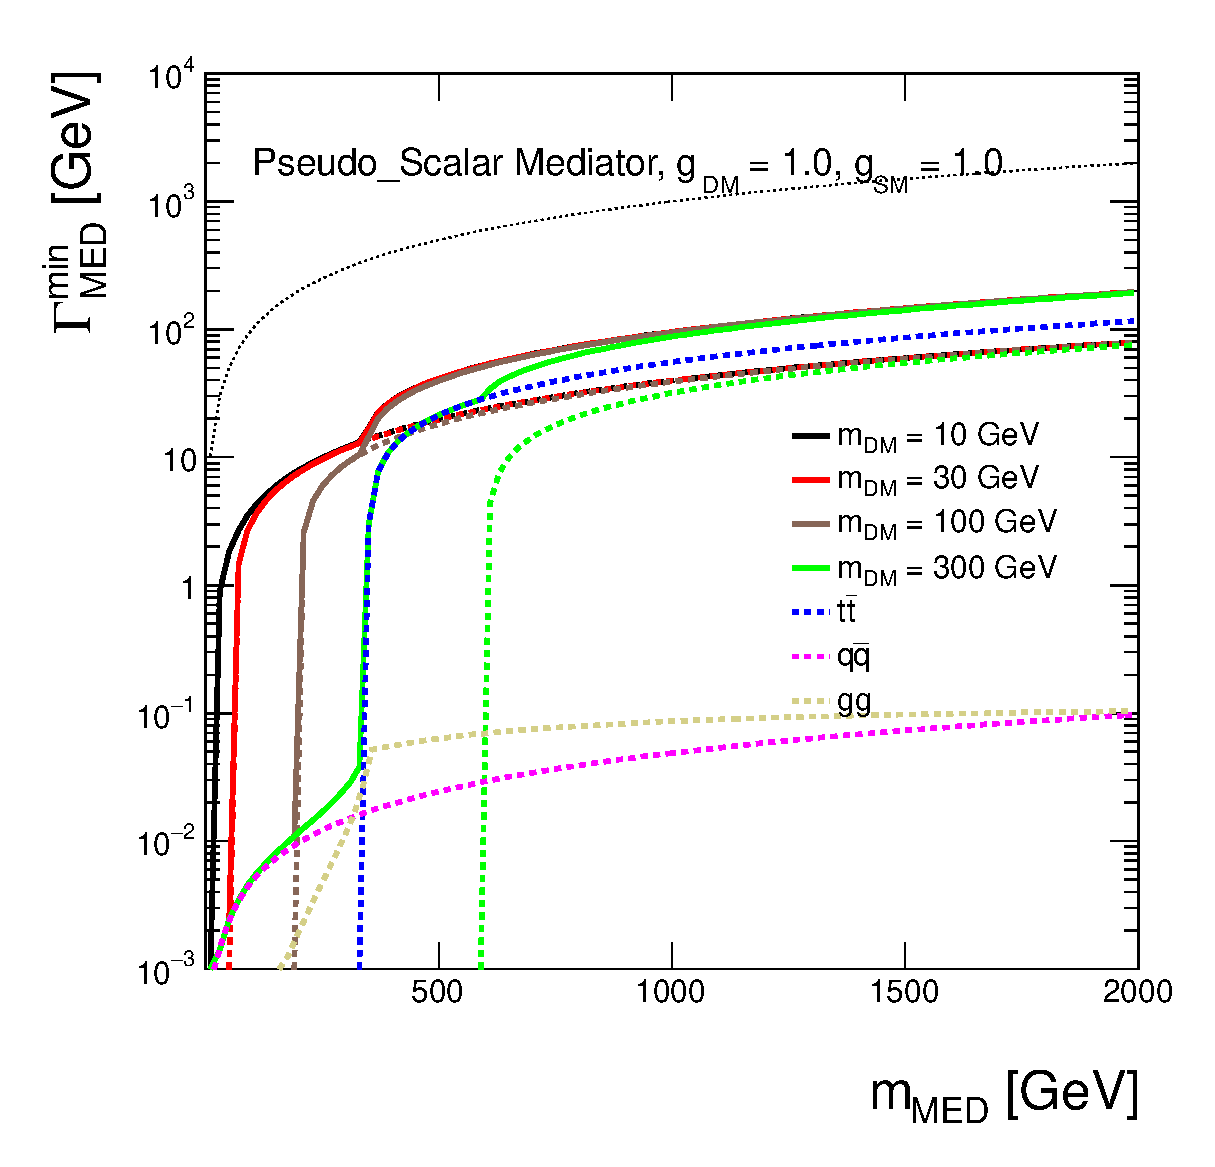
\includegraphics[width=0.95\textwidth]{figures/monojet/width_P.eps}
	\caption{Minimal width as a function of mediator mass for scalar and pseudo-scalar mediator assuming couplings of 1. The total width is shown as solid lines for Dark Matter masses of \mDM=10~\gev, 30~\gev, 100~\gev and 300~\gev in black, red, brown and green, respectively. The individual contributions from Dark Matter are indicated by dotted lines with the same colors. The contribution from all quarks but top is shown as magenta dotted line and the contribution from top quarks only is illustrated by the dotted blue line. The dotted beige line shows the contribution from the coupling to gluons. The dotted black line shows the extreme case $\Gamma_{\rm{min}}=\mMed$.}
	\label{fig:monojet_width_S}
\end{figure}

It can be seen in Fig.~\ref{fig:monojet_SPmodels} that the kinematics for the scalar and pseudoscalar models coincides when considering the diagrams in Fig.~\ref{fig:feyn_prod_S}. 
For this reason, we recommend to fully simulate only one of the two models.
%, and report the cross-sections on HEPData 
%for the other one.
No preference is given between the two models as they have the
same kinematics, although it is worth noting that the pseudo-scalar model has been used for a Dark Matter interpretation of the DAMA signal 
and of the galactic center excess~\cite{Arina:2014yna}.
Like in the case of the vector and axial-vector models described in Section~\ref{sec:monojet_spin}, the differences between the cross sections for the scalar and pseudo-scalar samples with the same $\mDM$ and $\mMed$ are increasing with the Dark Matter mass for fixed mediator mass, with the pseudo-scalar model yielding larger cross sections. There is an increasing difference between the minimal widths close to the $2\mDM=\mMed$ threshold.

\begin{figure*}
	\centering
	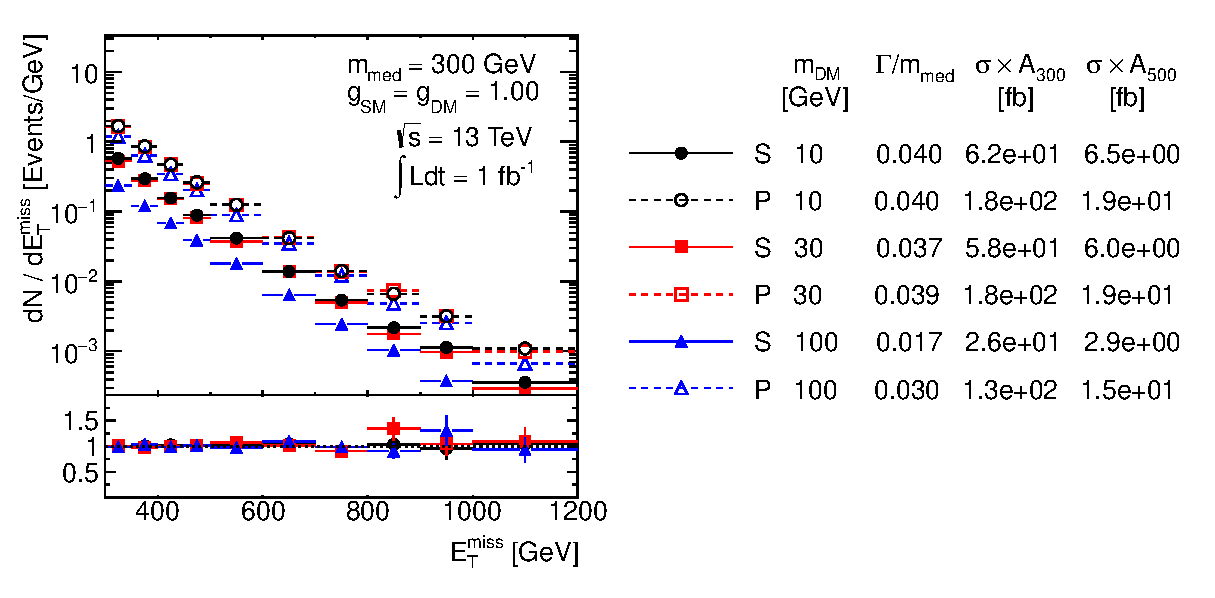
\includegraphics[width=0.95\textwidth]{figures/monojet/compareModels_SP_300.eps}
	\caption{Comparison of the $\MET$ distributions for the scalar and pseudoscalar models for different $\mMed=300\,\gev$ and different Dark Matter masses. 
		Ratios of the normalized distributions with respect to the first one are shown. $A_{300}$ and $A_{500}$ in the table denote the acceptance of the $\MET>300$~\gev and $\MET>500$~\gev cut, respectively.}
	\label{fig:monojet_SPmodels}
\end{figure*}

\subsubsection{Proposed parameter grid}

The optimized parameter grid in the $\mMed$--$\mDM$ plane for scalar and pseudo-scalar mediators is motivated by similar arguments as in the previous section. Therefore, a similar pattern is followed here, with the exception of taking $\gq=\gDM=1$. The choice of $\gq=0.25$ for the vector and axial-vector models is motivated by suppressing constraints from di-jets, which is not a concern in the scalar and pseudo-scalar mediator case. Here a di-jet signal emerges only at the 2-loop level through diagrams where the mediator is produced via gluon-gluon fusion and decays back into two gluons through a top loop. The strong loop suppression renders such signals unobservable at the LHC. Further constraints on the scalar and pseudo-scalar mediators may emerge from searches in $t\bar{t}$ final states. Studies of the electroweak effects to $t\bar{t}$ production suggest that one can only expect percent level contributions for $\gq \sim O(1)$ \cite{Haisch:2013fla}. Therefore, keeping $\gq=\gDM=1$ is a reasonable choice in the case of the scalar and pseudo-scalar mediators. Contrary to the vector and axial-vector models, note that couplings of 1 lead to $\Gamma_{\rm{min}}/\mMed \lsim 0.04$, ensuring the narrow width approximation is applicable. Furthermore, the sensitivity to the highest mediator masses has to be re-evaluated. The generator level cross section times the acceptance at $\MET>500$~\gev for the model with couplings $\gq=\gDM=1$, light Dark Matter of \mDM=10~\gev and a \mMed=500~\gev scalar mediator is at the order of 10\,fb, i.e. just at the edge of the early Run-2 sensitivity. Increasing the mediator mass to 1~\tev pushes the product $\sigma\times A$ down to approximately 0.1\,fb, below the LHC sensitivity. Therefore, we choose to remove the 2~\tev mediator mass from the grid and present the final grid with 33 mass points only, as shown in Tab.\,\ref{tab:mDMmMedScan_SP}. One point at very high mediator mass (10~\tev) is added for each of the DM masses scanned, to aid the reinterpretation of results in terms of contact interaction operators (EFTs).

\begin{table}[!h]
\centering
\begin{tabular}{| l |r r r r r r r r r|}
\hline
\multicolumn{1}{|c|}{\mDM (\gev)} & \multicolumn{9}{c|}{\mmed (\gev)} \\
\hline
 1             &         10  & 20 & 50 & 100 & 200 & 300 & 500 &         1000  &         10000  \\
 10   	       &         10  & 15 & 50 & 100 &     &     &     &               &         10000  \\
 50            &         10  &    & 50 &  95 & 200 & 300 &     &               &         10000  \\
 150           &         10  &    &    &     & 200 & 295 & 500 &         1000  &         10000  \\
 500           &         10  &    &    &     &     &     & 500 &          995  &         10000  \\
 1000          &         10  &    &    &     &     &     &     &         1000  &         10000  \\
\hline
\end{tabular}

\caption{Simplified model benchmarks for \schannel simplified models (\spinzero mediators 
decaying to Dirac DM fermions in the scalar and pseudoscalar case, taking the minimum width for \gq = 0.25 and \gDM = 1)}.
% Points in \textbf{bold} are only generated for the vector/axial vector cases, while points in 
% \textit{italics} are generated for the monojet analysis 
% but not for the search including heavy quarks. This table corresponds to 29 points for monojet vector/axial vector models,
% 26 points for monojet scalar/pseudoscalar models and 24 points for $t \bar{t}$+\MET scalar/pseudoscalar models.}

\label{tab:mDMmMedScan_SP}
% \end{sidewaystable}
\end{table}

% \begin{figure}
% \centering
% 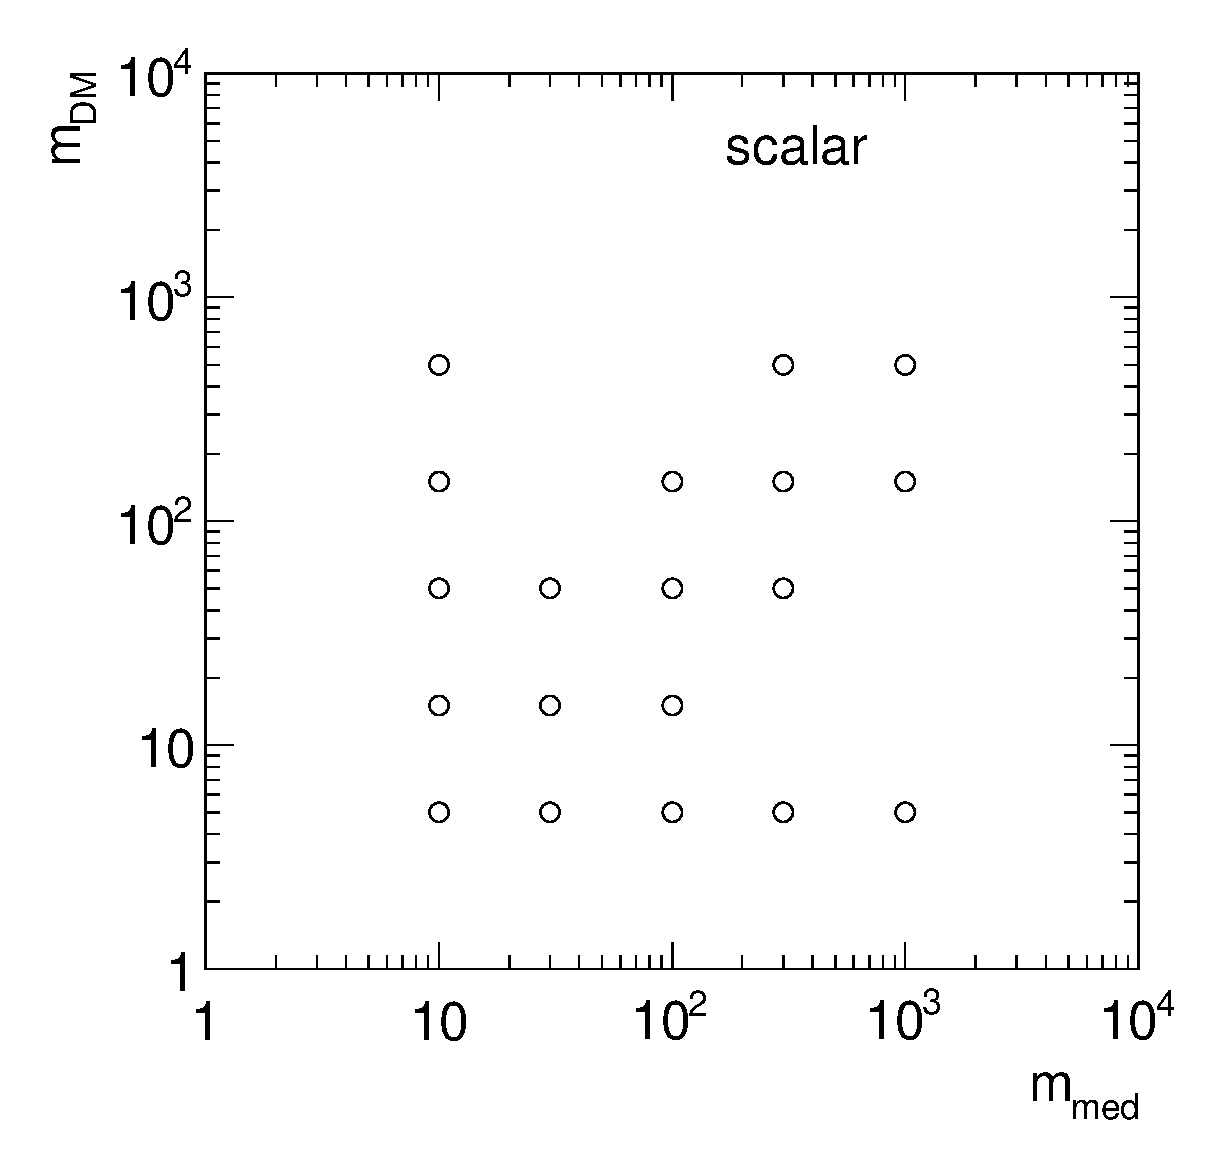
\includegraphics[width=0.95\textwidth]{figures/monojet/grid_S.eps}
% 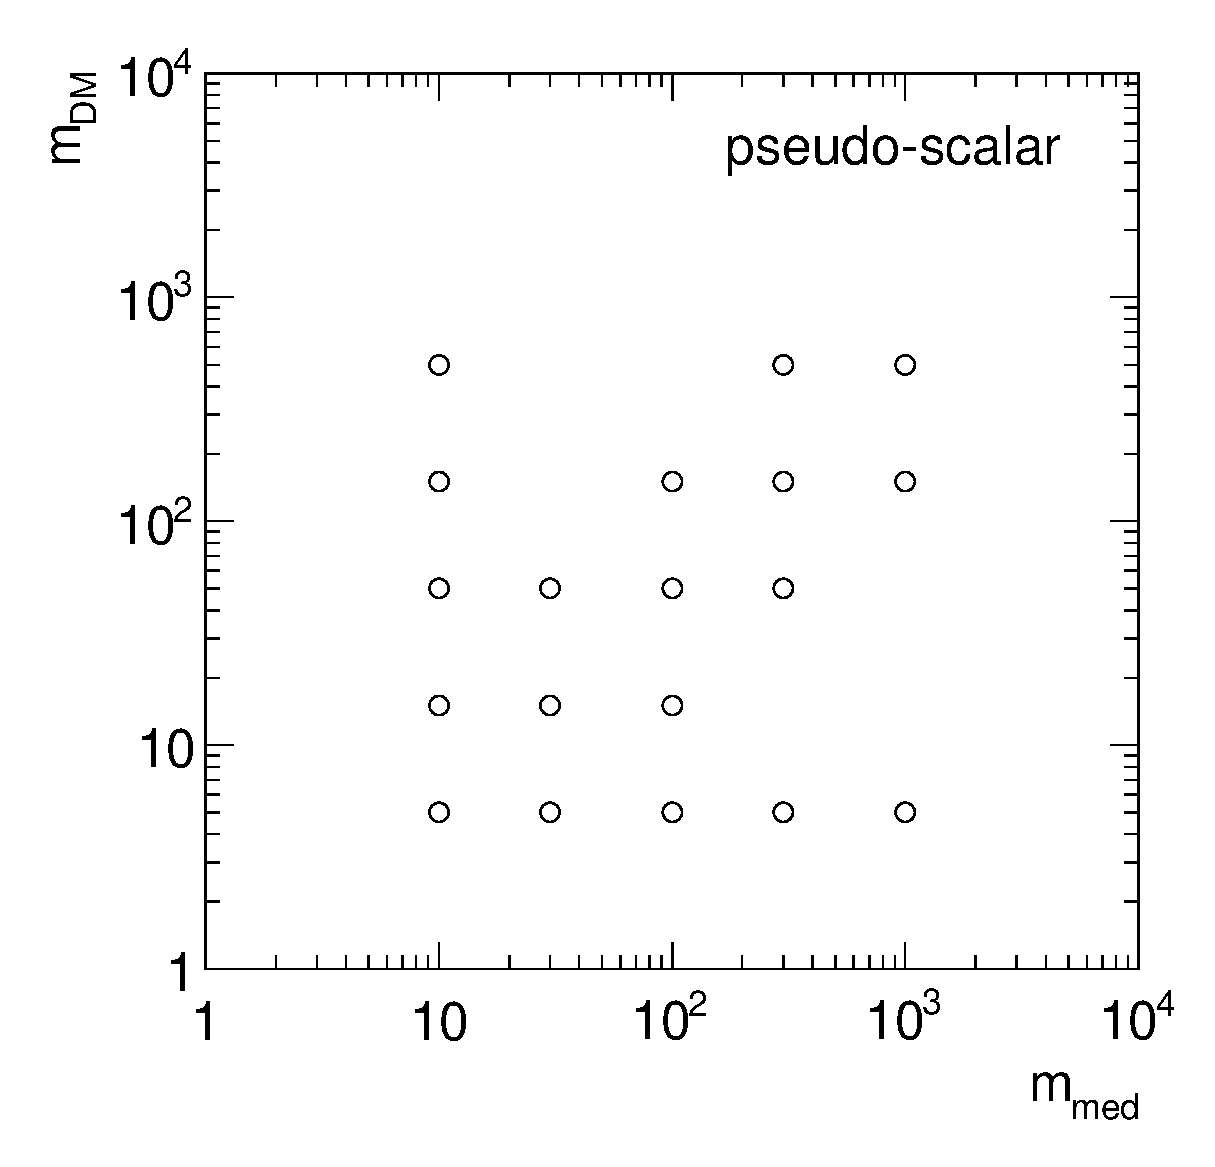
\includegraphics[width=0.95\textwidth]{figures/monojet/grid_P.eps}
% \caption{Proposed parameter grid for scalar and pseudo-scalar mediator in the $\mMed$--$\mDM$ plane.}
% \label{fig:monojet_grid_S}
% \end{figure}


For the parameter grid for scalar and pseudo-scalar mediator \schannel exchange, the $\Gamma_{\rm{min}}/\mMed$ ratio is given in Tables\,\ref{tab:widthS} and \ref{tab:widthP}, respectively. In the on-shell production regime, the ratio is $\sim0.04$. Very narrow resonances with $\Gamma_{\rm{min}}/\mMed<0.001$ correspond to the mass points where Dark Matter is produced off-shell. Note that the loop-induced contribution from gluons is ignored in the width calculation.


\begin{table}
	\centering
	\resizebox{\textwidth}{!}{
		\begin{tabular}{| l |r r r r r r r r r|}
			\hline
			\multicolumn{1}{|c|}{\mDM/\gev} & \multicolumn{9}{c|}{\mmed/\gev} \\
			&         10  & 20 & 50 & 100 & 200 & 300 & 500 &         1000  & 10000  \\
			\hline
			\hline
			1 & 0.040  & 0.040  & 0.040  & 0.040  & 0.040  & 0.040  & 0.041  & 0.043  & 0.043  \\
			10 &$<$0.001&$<$0.001& 0.040  & 0.040  &        &        &        &        & 0.043  \\
			50 &$<$0.001&        &$<$0.001&$<$0.001& 0.040  & 0.040  &        &        & 0.043  \\
			150 &$<$0.001&        &        &        &$<$0.001&$<$0.001& 0.041  & 0.043  & 0.043  \\
			500 &$<$0.001&        &        &        &        &        & 0.001  & 0.003  & 0.043  \\
			1000 &$<$0.001&        &        &        &        &        &        & 0.003  & 0.043  \\
			\hline
		\end{tabular}}
		\caption%[][5cm]
		{Minimal width of the scalar mediator exchanged in \schannel divided by its mass, assuming $\gq=0.25$ and $\gDM=1$. The loop-induced gluon contribution is ignored. The numbers tabulated under $2\mDM=\mMed$ correspond to the width calculated for $\mMed-5$~\gev.}
		\label{tab:widthS}
	\end{table}
	\vspace{4cm}
	
	
	\begin{table}
		\centering
		\resizebox{\textwidth}{!}{
			\begin{tabular}{| l |r r r r r r r r r|}
				\hline
				\multicolumn{1}{|c|}{\mDM/\gev} & \multicolumn{9}{c|}{\mmed/\gev} \\
				&         10  & 20 & 50 & 100 & 200 & 300 & 500 &         1000  & 10000  \\
				\hline
				\hline
				1 & 0.040  & 0.040  & 0.040  & 0.040  & 0.040  & 0.040  & 0.042  & 0.043  & 0.043  \\
				10 &$<$0.001&$<$0.001& 0.040  & 0.040  &        &        &        &        & 0.043  \\
				50 &$<$0.001&        &$<$0.001&$<$0.001& 0.040  & 0.040  &        &        & 0.043  \\
				150 &$<$0.001&        &        &        &$<$0.001&$<$0.001& 0.042  & 0.043  & 0.043  \\
				500 &$<$0.001&        &        &        &        &        & 0.003  & 0.003  & 0.043  \\
				1000 &$<$0.001&        &        &        &        &        &        & 0.003  & 0.043  \\
				\hline
			\end{tabular}}
			\caption%[][5cm]
			{Minimal width of the pseudo-scalar mediator exchanged in \schannel divided by its mass, assuming $\gq=0.25$ and $\gDM=1$. The loop-induced gluon contribution is ignored. The numbers tabulated under $2\mDM=\mMed$ correspond to the width calculated for $\mMed-5$~\gev.}
			\label{tab:widthP}
		\end{table}
		\vspace{4cm}
		


\subsection{Additional considerations for $V+\MET$ signatures}
\label{sub:EW_Scalar}

The discussion of parameters for the model with a color-singlet, \spinzero mediator
parallels that in Section~\ref{subsec:MonojetLikeModels}. 

Even though the sensitivity of mono-boson searches to this model is low and it may not
be in reach of early LHC searches, this model can be generated for W, Z and photon searches 
in order to reproduce the kinematics of contact interaction operators that are further 
described in Section~\ref{sub:EW_EFT_Dim5}, to aid later reinterpretation.  

%\subsection{Model implementation}
%
%These models are generated at leading
%order with \madgraph 2.2.2, using Pythia8 for the parton shower.
%Parameter cards can be found on the Forum SVN repository~\cite{ForumSVN_EW_DMV}.
%\Todo{Add models and instructions for other final states}.

\subsection{\texorpdfstring{Additional considerations for $t \bar{t}$ and $b \bar{b}$+\MET signatures}{Additional considerations for ttbar/bbbar+\MET signatures}}
\label{subsec:DMHFModels}
\svnidlong
{$HeadURL$}
{$LastChangedDate$}
{$LastChangedRevision$}
{$LastChangedBy$}
\svnid{$Id$}

%As described in Section~\ref{sec:monojet_scalar}, a model with a scalar/pseudoscalar particle 
%mediating the DM-SM interactions is one of the simplest UV completions of our EFT models.  
With the MFV assumption, the top and bottom
quark can play an important  role in the phenomenology.
The scalar and pseudoscalar mediator models predict not only
the monojet process described in Section~\ref{sec:monojet_scalar}, but also production of Dark Matter
in association with top (or bottom) pairs, as illustrated in Fig.~\ref{fig:TTbarPhi}. 
Dedicated searches including jets from heavy flavor quarks in the final state
can be designed for this signature. Another class of simplified models,  
which includes a Dark Matter interpretation among many others, and yields a single
top quark in the final state, is detailed in Appendix~\ref{sec:singletop}. 

\begin{figure}[h!]
\centering
  \unitlength=0.005\textwidth
  \begin{feynmandiagram}[modelTTbarMET]
    \fmfleft{i1,i2}
    \fmfright{o1,o4,o5,o3}
    \fmf{gluon}{i1,v1}
    \fmf{gluon}{i2,v2}
    \fmf{fermion}{o1,v1,v3,v2,o3}
    \fmf{scalar}{v3,v4}
    \fmf{fermion}{o5,v4,o4}
    \fmf{phantom,tension=0,label={$\phi/a$}}{v3,v4}    
    \fmflabel{\Large $g$}{i1}
    \fmflabel{\Large $g$}{i2}
    \fmflabel{\Large $t (b)$}{o1}
    \fmflabel{\Large $\bar t (\bar b)$}{o3}
    \fmflabel{\Large $\chi$}{o4}
    \fmflabel{\Large $\bar \chi$}{o5}    
  \end{feynmandiagram}
%\caption[][\baselineskip]{Representative Feynman
\caption{Representative Feynman
diagram showing the pair production of Dark Matter particles in
association with $t\bar t$ (or $b\bar b$).}
\label{fig:TTbarPhi}
\setfloatalignment{t}
\end{figure}

%\section{Specific models involving $b-$ quarks in the final state}

In addition to the $t\bar t$+DM models illustrated in Fig.~\ref{fig:TTbarPhi}, 
some theoretically motivated scenario (e.g. for high $tan\beta$ in 2HDM in the pMSSM) 
privilege the coupling of \spinzero mediators to down generation quarks.
This assumption motivates the study of final states involving $b$-quarks 
as a complementary search to the $t\bar
t$+DM models, to directly probe the $b$-quark coupling. 
An example of such a model can be found in Ref.~\cite{Buckley:2014fba}
and can be obtained by replacing top quarks with $b$ quarks in Fig.~\ref{fig:TTbarPhi}.
Note that, because of the kinematics features of $b$ quark production relative
to heavy $t$ quark production, a $b\bar b$+DM final state may only yield one
experimentally visible $b$ quark, leading to a mono-$b$ signature in a model that conserves $b$ flavor.

Dedicated implementations of these models for the work of this Forum are available at LO+PS accuracy,
even though the state of the art is set to improve on a timescale beyond that for early Run-2 DM searches
as detailed in Section~\ref{sec:TTBar_implementation}.
The studies in this Section have been produced using a leading order UFO model within \madgraph 2.2.2
~\cite{Alwall:2014hca,Alloul:2013bka,Degrande:2011ua} 
using \pythiaEight for the parton shower. 

\subsubsection{Parameter scan}

%As discussed in Sec.~\ref{subsec:MonojetLikeModels}, the MFV and universal coupling assumptions for \spinzero
%mediators lead to quark mass dependent Yukawa couplings and therefore dominant couplings to top quarks.

The parameter scan for the dedicated $t\bar{t}$+\MET{} searches has been studied in detail to target the production 
mechanism of DM associated with heavy flavor quarks, and shares many details of the scan for the scalar model with a gluon radiation.
The benchmark points scanning the model parameters have been selected to ensure that the kinematic features of the 
parameter space are sufficiently represented. Detailed studies were performed to identify points in the \mdm, 
$m_{\phi,a}$, $\gDM$, $\gq$ (and $\Gamma_{\phi,a}$) parameter space that differ significantly from each other 
in terms of expected detector acceptance. Because missing transverse momentum is the key observable for searches, the 
mediator $p_{T}$ spectra is taken to represent the main kinematics of a model. Another consideration in determining the set 
of benchmarks is to focus on the parameter space where we expect the searches to be sensitive during the 2015 LHC run. 
Based on a projected integrated luminosity of $30\,{\rm fb}^{-1}$ expected for 2015, we disregard model points with a 
cross section times branching ratio smaller than $0.1\,{\rm fb}$, corresponding to a minimum of one expected event 
assuming a 0.1\% efficiency times acceptance. 

The kinematics is most dependent on the masses \mdm and $m_{\phi,a}$. Figure~\ref{fig:scanPhi} 
and~\ref{fig:scanPhiPseudo} show typical dependencies for scalar and pseudoscalar couplings respectively.
Typically, the mediator $p_T$ spectrum broadens with larger $m_{\phi,a}$. 
The kinematics are also different between on-shell ($\mMed>2\mdm$) and off-shell ($\mMed<2\mdm$) mediators as discussed in Section~\ref{sec:monojet_scalar}. 
Furthermore, the kinematic differences in the \MET{} spectrum between scalar and pseudoscalar are larger for light mediator 
masses with respect to heavier mediators. It is therefore important to  
choose benchmark points covering on-shell and off-shell mediators with sufficient granularity, including the
transition region between on-shell and off-shell mediators. %, as inFig.~\ref{fig:scanPhidiag}. 

\begin{figure}[!ht]
  \begin{center}
    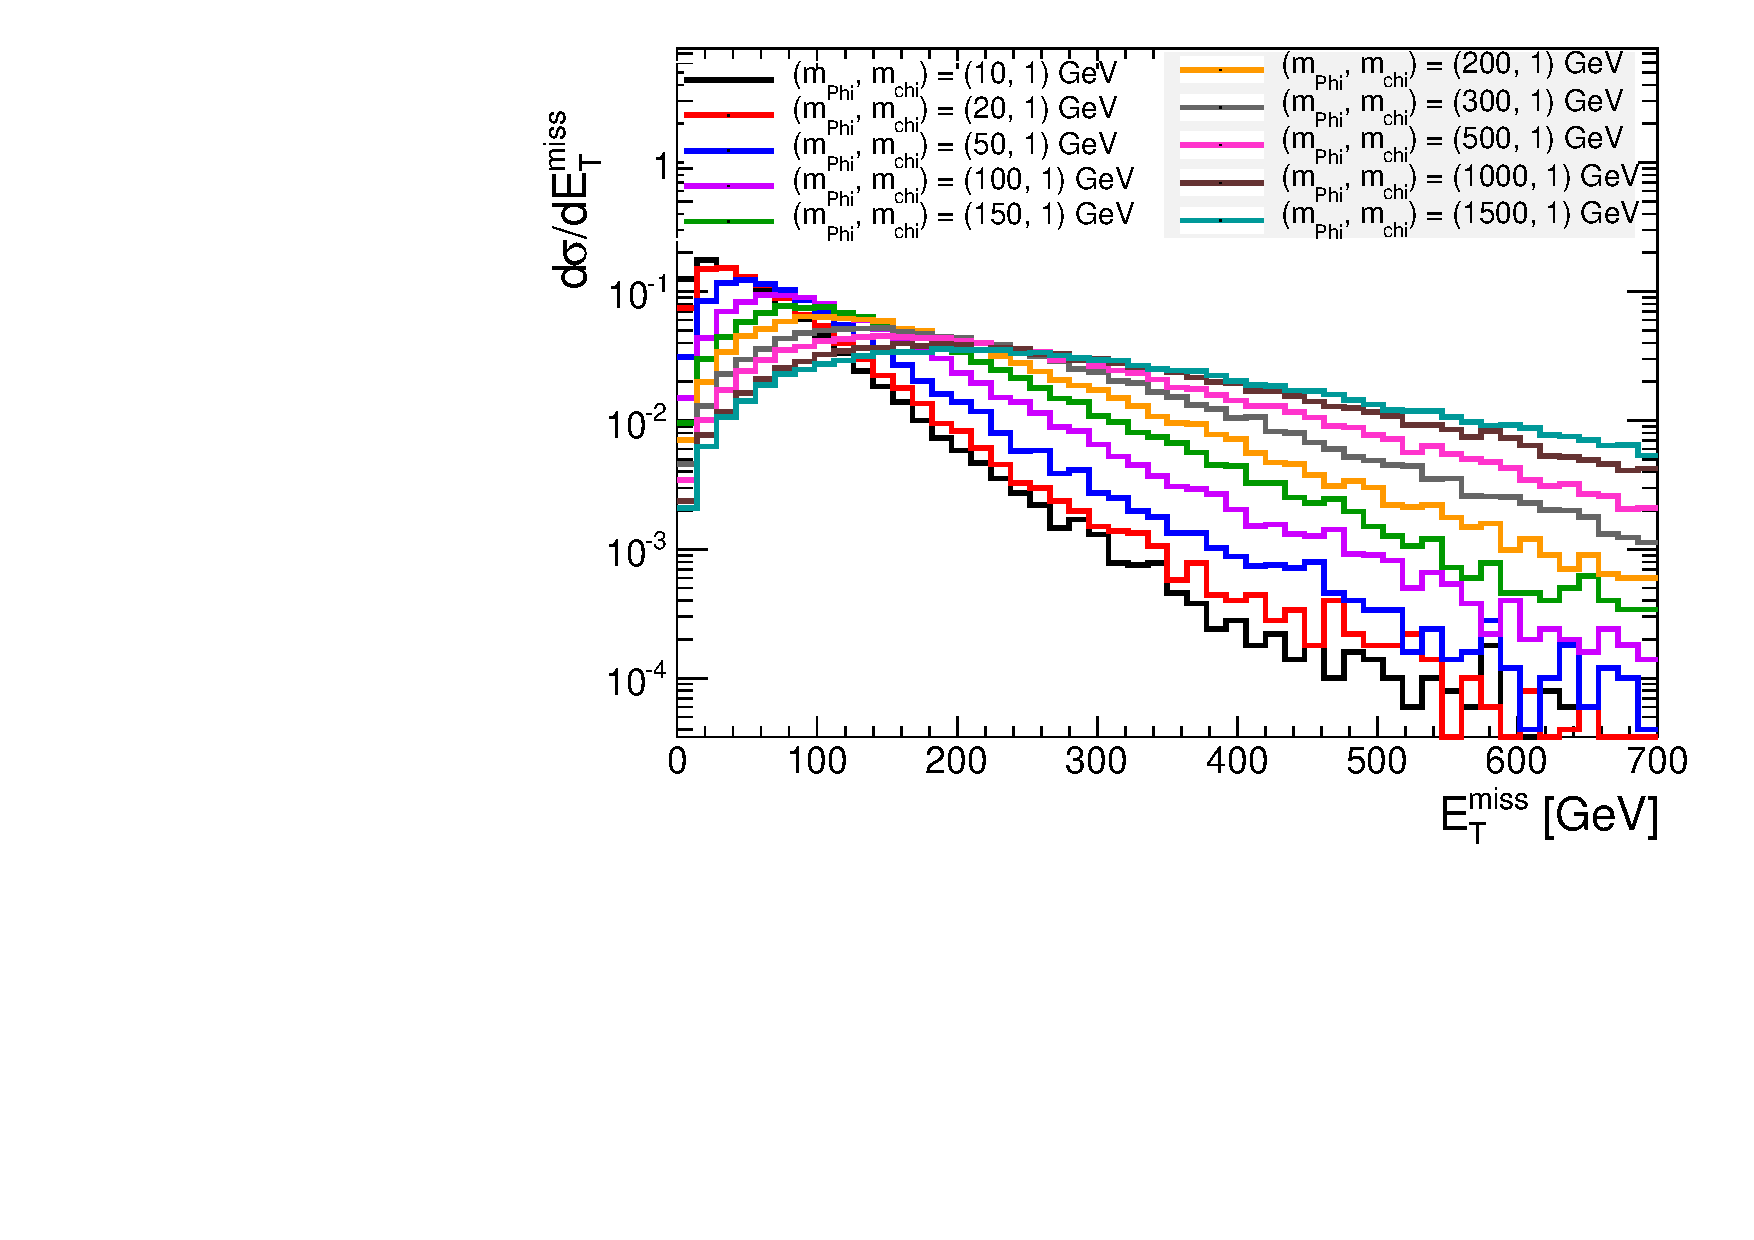
\includegraphics[width=0.95\textwidth]{figures/ttbar/MEt_chi1.pdf}
    \caption{\label{fig:scanPhi} Example of the dependence of the kinematics on the scalar mediator mass in the $t\bar{t}$+\MET{} signature. The Dark Matter mass is fixed to be \mdm=$1 {\rm GeV}$.}
\end{center}
\end{figure}


\begin{figure}[!ht]
  \begin{center}
    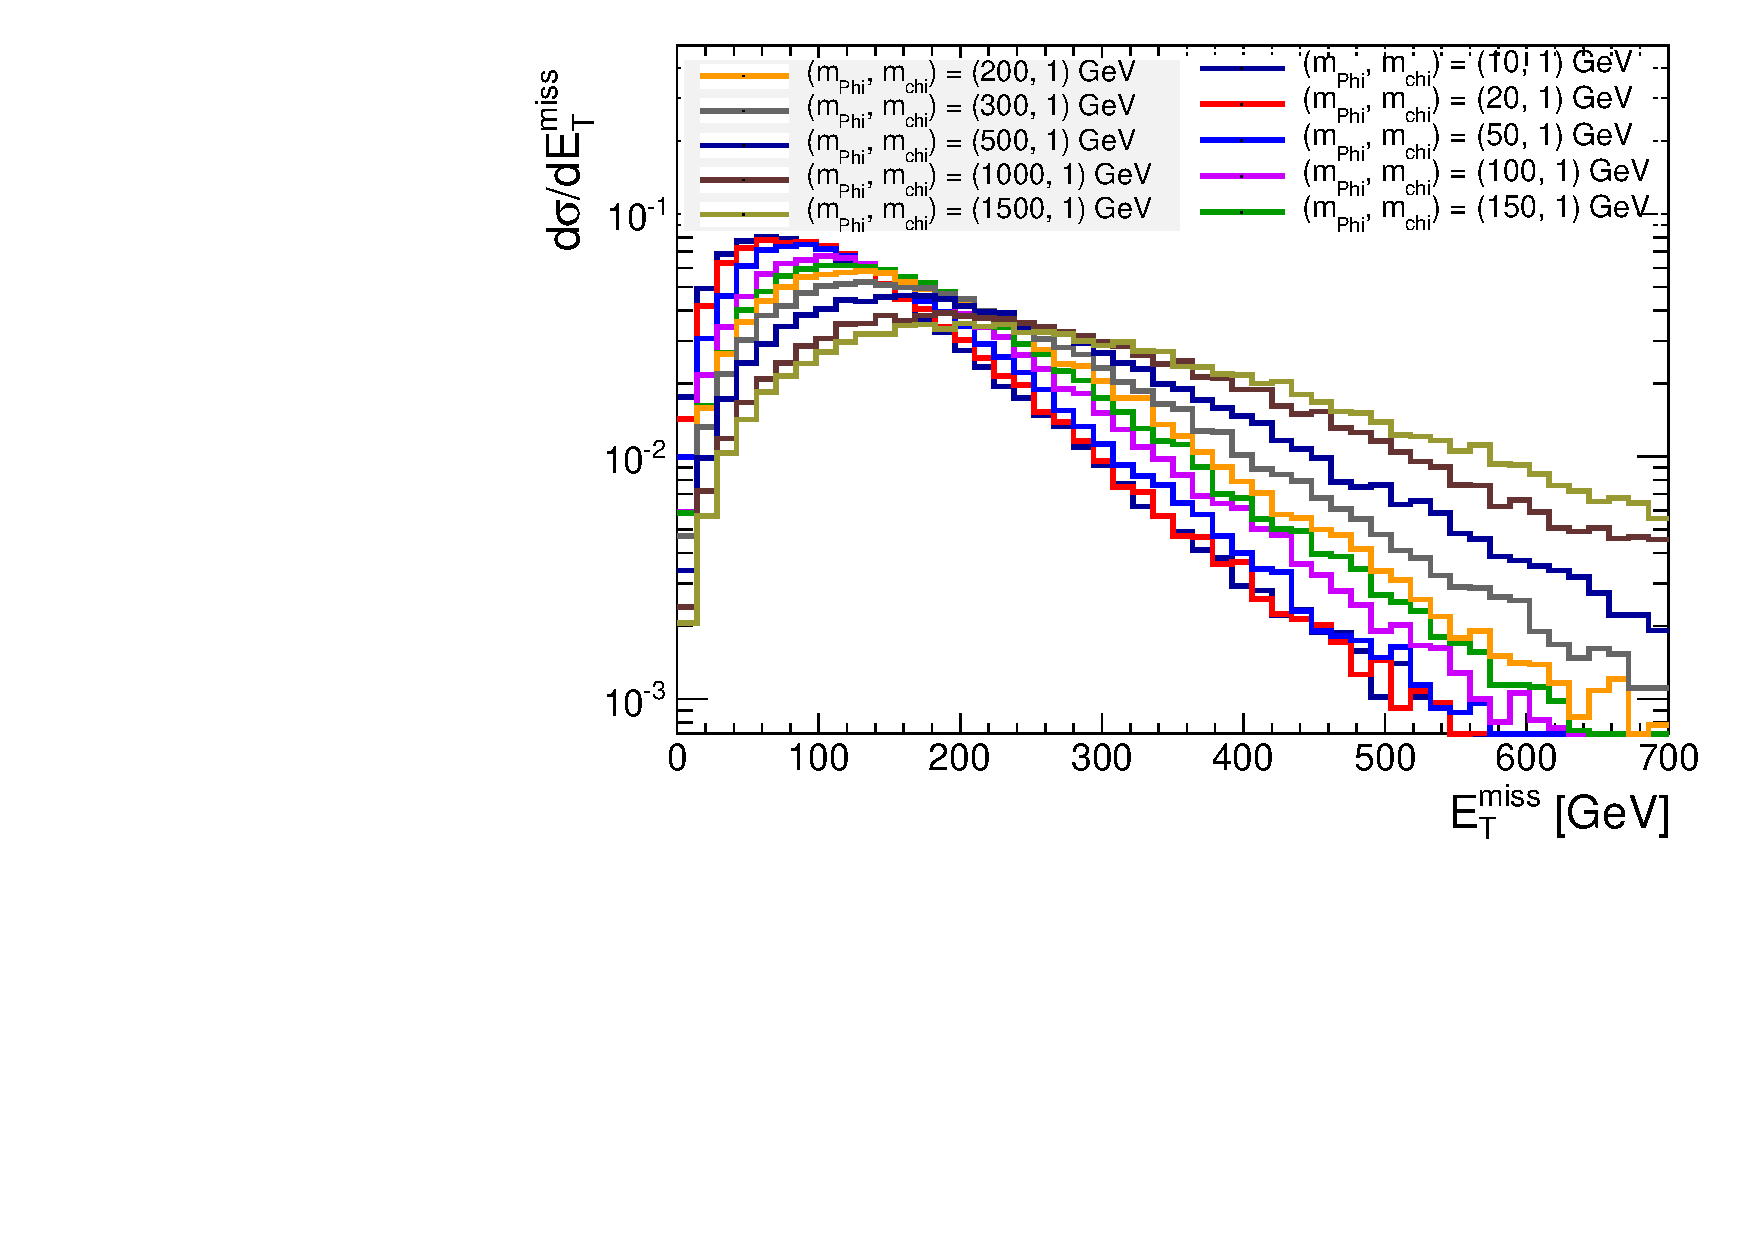
\includegraphics[width=0.95\textwidth]{figures/ttbar/MEt_chi1_pseudo.pdf}
    \caption{\label{fig:scanPhiPseudo} Example of the dependence of the kinematics on the pseudoscalar mediator mass in the $t\bar{t}$+\MET{}. The Dark Matter mass is fixed to be \mdm=$1 {\rm GeV}$. All figures concerning the $t\bar{t}$+\MET{}  signature have been produced using a leading order model within \madgraph 2.2.2, using \pythiaEight for the parton shower.}
\end{center}
\end{figure}

%\begin{figure}[!ht]
%  \begin{center}
%    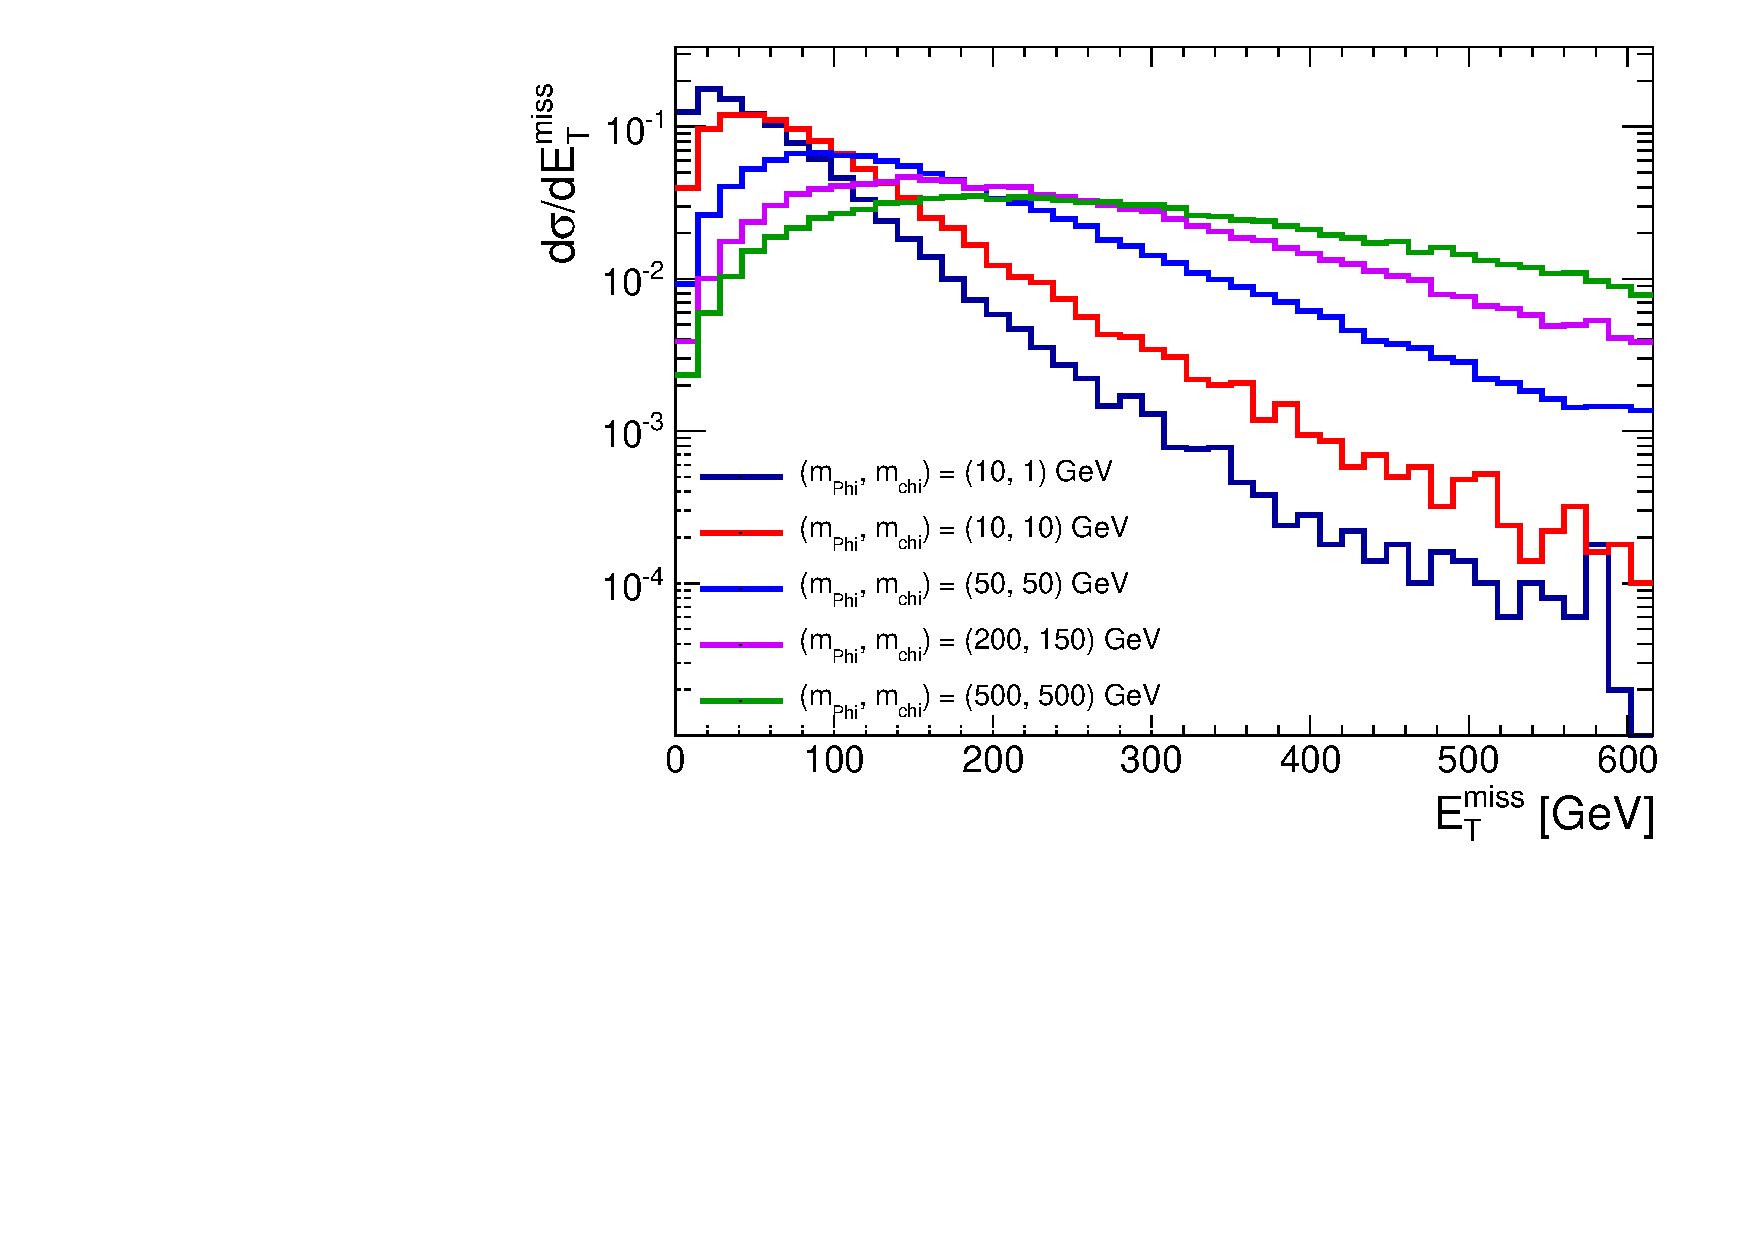
\includegraphics[width=0.95\textwidth]{figures/ttbar/MEt_diagonal_scan.pdf}
%    \caption{\label{fig:scanPhidiag} Example of the dependence of the kinematic for points of the grid proposed in Tab.~\ref{sec:monojet_scalar} close to the $m_{\phi,a} \sim 2m_\chi$ limit.
%    }
%\end{center}
%\end{figure}

Typically only weak dependencies on couplings are observed (see Fig~\ref{fig:widthsmallscan}) where the variation with width of the integral over parton distributions is unimportant. As shown in Section~\ref{sub:parameter_scan_monojet}, for couplings $\sim O(1)$ the width is large enough that the $p_T$ of the mediator is determined mainly by the PDF. 

At large mediator masses ($\sim 1.5\,{\rm TeV}$) or very small couplings ($\sim 10^{-2}$), width effects are significant, but these regimes have production cross sections that are too small to be relevant for $30\,{\rm fb}^{-1}$ and are not studied here. However, with the full Run~2 dataset, such models may be within reach. 

\begin{figure}[!ht]
  \begin{center}
    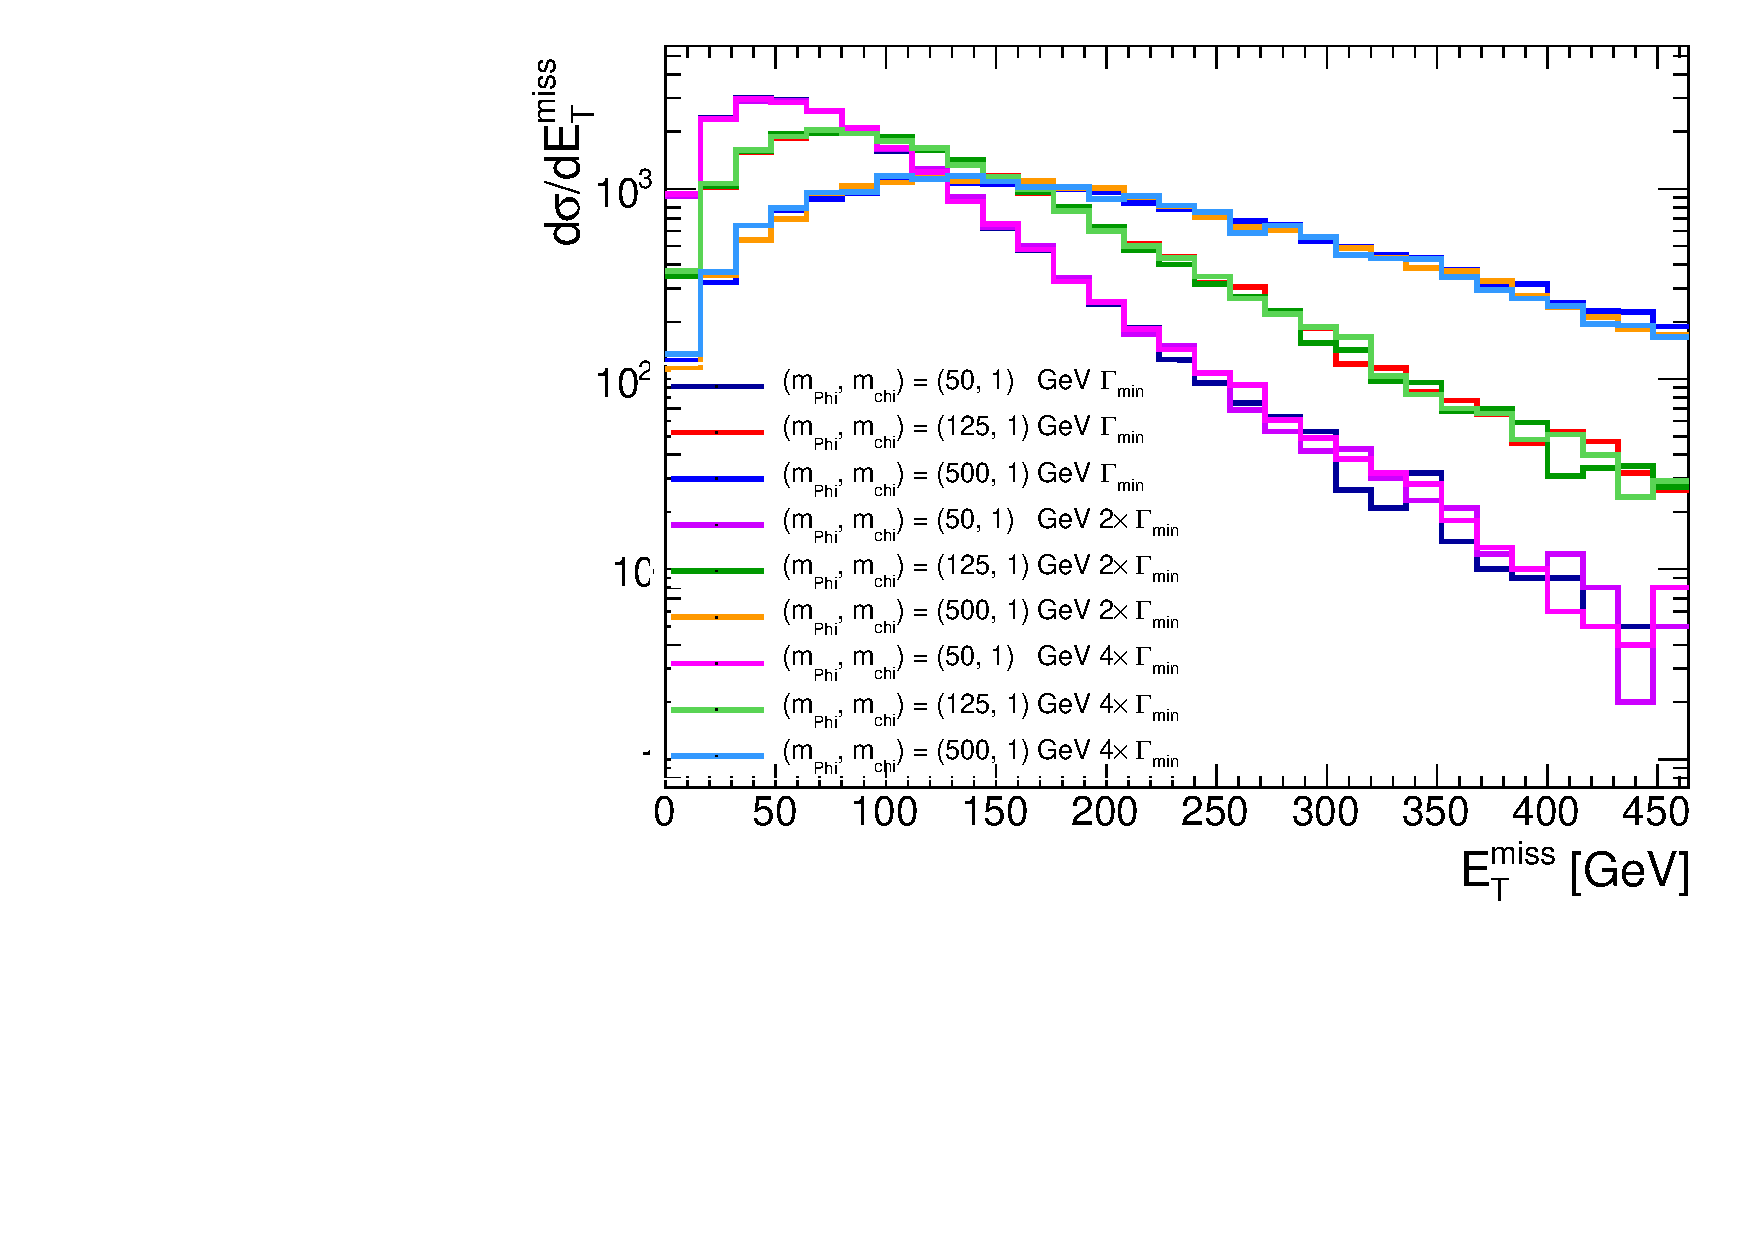
\includegraphics[width=0.95\textwidth]{figures/ttbar/MEt_smallwidth.pdf}
    \caption{\label{fig:widthsmallscan} Study of the dependence of kinematics on the width of a scalar mediator $t\bar{t}$+\MET{}. The width is increased up to four times the minimal width for each mediator and Dark Matter mass combination. 
    }
\end{center}
\end{figure}

Another case where the width can impact the kinematics is when $m_{\phi,a}$ is slightly larger than $2m_\chi$. Here, the width determines the relative contribution between on-shell and off-shell mediators. An example is given in Fig.~\ref{fig:widthlargescan}. As the minimal width choice pursued in this document is the most conservative one, this effect can be neglected in order to reduce the number of benchmark points to be generated. 

%In our recommendations we propose to use for simplicity the minimal width, as this is represents the most conservative choice to interpret the LHC results. 

\begin{figure}[!ht]
  \begin{center}
    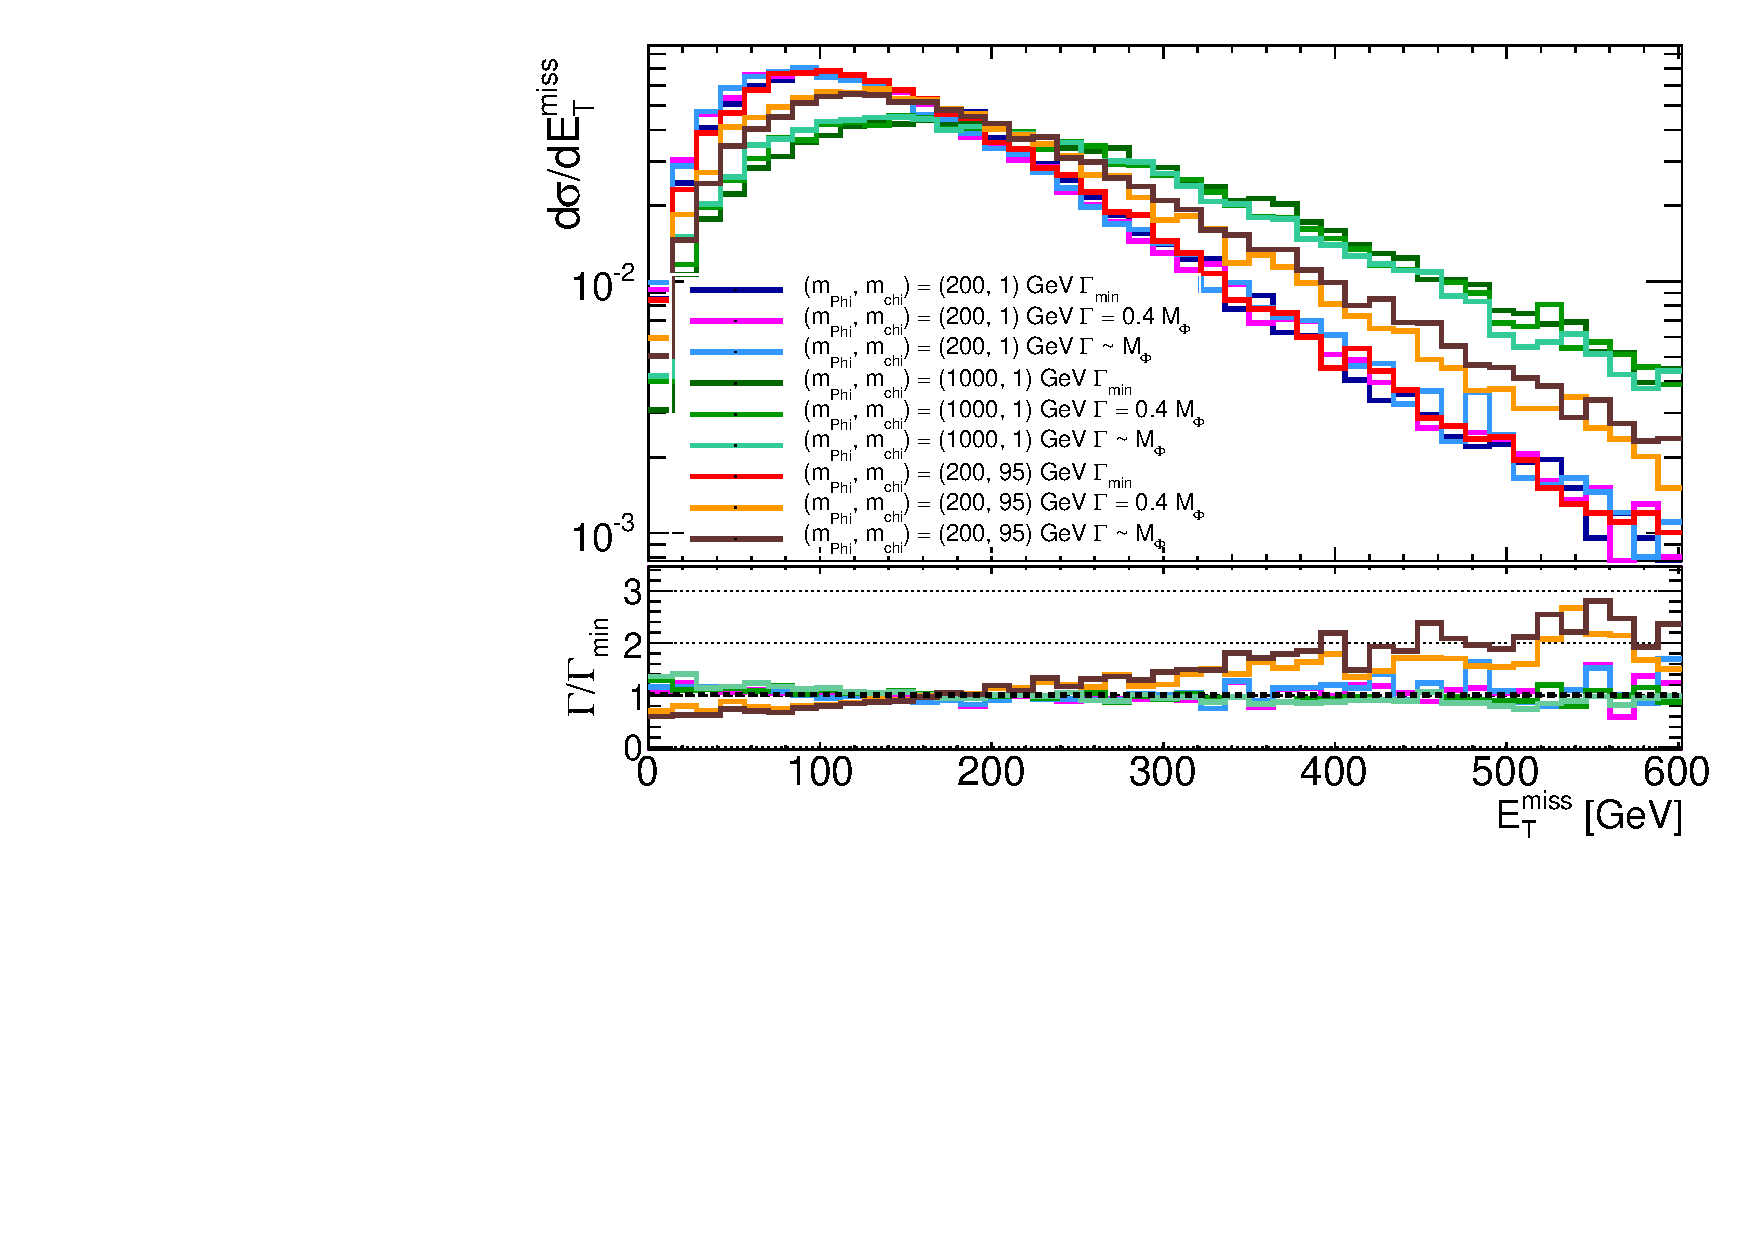
\includegraphics[width=0.95\textwidth]{figures/ttbar/ScalarWidth.pdf}
    \vspace{2mm}
    \caption{\label{fig:widthlargescan} Dependence of the kinematics on the width of a scalar mediator $t\bar{t}$+\MET{}. The width is increased up to the mediator mass. Choices of mediator and Dark Matter masses such that $m_{\phi,a}$ is slightly larger than $2m_\chi$ is the only case that shows a sizeable variation of the kinematics as a function of the width.  
    }
\end{center}
\end{figure}

The points for the parameter scan chosen for this model are listed in Table~\ref{tab:mDMmMedScan_SP}, chosen
to be harmonized with those for other analyses employing the same scalar model as benchmark. 
Based on the sensitivity considerations above, DM masses are only simulated up to 500 GeV (but the 5 TeV mediator point is retained)
leading to a total of 24 benchmark points. However for these searches we recommend to generate and simulate scalar and pseudoscalar
models separately, as the kinematics differs due to the different coupling of the mediator to the final state top quarks in the two cases,
as shown in Figs.~\ref{fig:scanPhi} and ~\ref{fig:scanPhiPseudo}.

Similar studies were performed in the $b \bar b$ case. It was found that they 
show the same weak dependence of the kinematics of the event on the mediator width.
The same benchmark parameters of the $t\bar t$ case could then be chosen.

%%
%[24/05/15 23:48:07] Caterina Doglioni: the plots are made with 5F, while we recommend 4F scheme
%[24/05/15 23:49:04] Caterina Doglioni: even though the relevant parameters do not change 
%(there are some plots due in the appendix for that, albeit with limited statistics), she doesn’t want to put them in 
%and wouldn’t be able to remake them with the right flavor scheme.

% Plots for bbar, if they make it
% Removing these plots as they won't make it last-minute. 
%\Todo{[TODO: The following figures are placeholders for now and will be added later].  If these are supporting material for the MC generation, put in the appendix}.
%
%\begin{figure}
%    \vbox{\hfill}
%    \caption{\label{fig:bbscanPhi} Example of the dependence of the kinematics on the scalar mediator mass. 
%    	The Dark Matter mass is fixed to be $1 {\rm GeV}$.}
%\end{figure}
%
%\begin{figure}[!ht]
%    \vbox{\hfill}
%    \caption{\label{fig:bbscanPhiPseudo} Example of the dependence of the kinematics on the pseudoscalar mediator mass. 
%    	The Dark Matter mass is fixed to be $1 {\rm GeV}$.}
%\end{figure}


%\newthought{Implementation}
%There are some subtleties to the Monte Carlo simulation relevant for
%this case that are discussed in Section~\ref{app:MonojetLikeModels_Appendix}.

%In addition to the considerations discussed in the preceding subsections, very light DM fermions are included ($\mdm=10\,{\rm GeV}$) 
%as this is a region where colliders have a complementary sensitivity to current direct detection experiments. 
% 
% \begin{table}[!ht]
% \centering
% \begin{tabular}{| l | r |}
% \hline
% \multicolumn{1}{|c|}{\mdm (${\rm GeV}$)} & \multicolumn{1}{c|}{$m_{\phi,a}$ (${\rm GeV}$)} \\
% \hline
%  $1$    & $10$, $20$, $50$, $100$, $150$, $200$, $300$, $500$, $1000$, $1500$  \\
%  $10$   & $10$, $20$, $50$, $100$, $150$, $200$, $300$, $500$, $1000$, $1500$  \\
%  $50$   &             $50$, $100$, $150$, $200$, $300$, $500$, $1000$, $1500$  \\
%  $150$  &                          $150$, $200$, $300$, $500$, $1000$, $1500$  \\
%  $500$  &                                               $500$, $1000$, $1500$  \\
% \hline
% \end{tabular}
% \caption{Simplified model benchmarks for $t\bar{t}$+DM production via \spinzero mediators decaying to Dirac DM fermions taking the minimum width presciption for $g_v = \gDM = 1$.}
% \label{tab:ttdm_benchmarks}
% \end{table}
% 


%%%%%%%%%%%%%%%%%
%%%%%%%%%%%%%%%%%
%%%%%%%%%%%%%%%%%
%%%%%%%%%%%%%%%%%
%%%%%%%%%%%%%%%%%
%%%%%%%%%%%%%%%%%
%%%%%%%%%%%%%%%%%

\section{Colored scalar mediator, \tchannel exchange}
\label{sec:monojet_t_channel}
\input tex/TChannelModels.tex

\section{ \Spintwo mediator}
\label{sec:spintwo}

In models with extra dimensions, the Kaluza-Klein excitations of the graviton could also serve as a mediator between the Standard Model and dark sector physics. This kind of model was not studied in the forum and is not included in the recommendations, but models such as Ref.~\cite{Lee:2013bua} may warrant further study on a longer timescale. 

% \begin{figure}
%   \centering
%   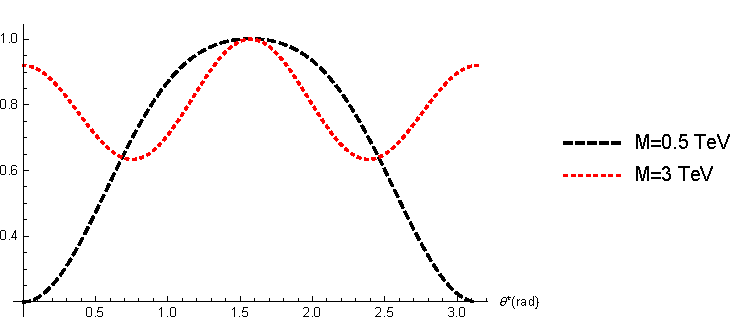
\includegraphics[width=\linewidth]{figures/monojet/comparison_G_mDM10.pdf}
%   \caption{Angular distributions of the total production for 0.5~\tev and 3~\tev graviton mediators for $\mDM=10$~\gev.}
% \end{figure}

% Below a few~\tev in mediator mass, production of a graviton with universal couplings is dominantly gluon-initiated. For heavy mediators, however, up to half of the production occurs through a qq-initiated diagram, leading to a large forward-peaked component of the production \cite{Allanach:2002gn}. For example, Fig.~\ref{fig:gravitoncomparison} shows a calculation of the angular distributions of the total production for 0.5~\tev and 3~\tev graviton mediators in the light WIMP limit ($\mDM=10$~\gev). 

%The proposal for the scan in the $\gq$--$\gDM$ plane is described in the following section.

\section{Presentation of results for reinterpretation of \schannel mediator models}
\label{sec:monojet_scaling}

The aim of the parameter grid optimization done for the \schannel models in the previous sections is to reduce the parameter space that must be simulated.  We then need a procedure for populating the full parameter space by using the simulated grid points.  We recommend doing this as follows:

\begin{itemize}
\item When the dependences on parameters are known, the cross
  sections and efficiencies at general points can be calculated from
  the grid data.
\item In other cases, this information can be obtained by interpolation
  between the grid points.  We have chosen the grid points so that the
  dependence is sufficiently smooth that this will be possible.
\end{itemize}

The results of the scan over the couplings presented in the previous sections indicate that there are no changes in kinematic distributions for different choices of the coupling strengths. This means that the acceptance remains the same in the whole $\gq$--$\gDM$ plane and it is sufficient to perform the detector simulation only for one single choice of $\gq, \gDM$. The resulting truth-level selection acceptance and the detector reconstruction efficiency can then be applied to all remaining grid points in the $\gq$--$\gDM$ plane where only the generator-level cross section needs to be known. This significantly reduces the computing time as the detector response is by far the most CPU-intensive part of the Monte Carlo sample production.
However, the number of generated samples can be reduced even further
if a parameterization of the cross section dependence from one grid point to another exists.
In this section, we describe the details of a cross section scaling procedure that
can be used to reinterpret results for a fixed coupling for \schannel mediator models.

The propagator for the \schannel exchange is written in a Breit-Wigner
form as $\displaystyle \frac{1}{q^2-\mMed^2 + i\mMed\Gamma}$, where $q$ is the momentum transfer calculated from the two partons entering the hard process after the initial state radiation, which is equivalent to the momentum of the Dark Matter pair~\footnote{Using a running width and replacing the denominator of the propagator with $q^2 - \mMed^2 + \complexi\,Q^2\,\frac{\Gamma}{\mMed}$ should be considered in the case of wide mediators~\cite{Bardin:1989qr}.}. %The relative size of the center-of-mass energy defined by the two partons entering the hard process and the mediator mass allows us to classify the production in the following way:
The size of the momentum transfer with respect to the mediator mass allows us to classify the production in the following way:
\begin{itemize}
	\item off-shell production when $q^2 \gg \mMed^2$ leading to suppressed cross sections,
	\item on-shell production when $q^2 \sim \mMed^2$ leading to enhanced cross sections,
	\item effective field theory (EFT) limit when $q^2 \ll \mMed^2$.
\end{itemize}
%All three categories can be distinguished in Fig.\,\ref{fig:monojet_MstarMmed} showing the upper limit on the interaction scale $M^{*} \equiv \mMed/\sqrt{\gq\gDM}$ for vector mediator. 
In the case of the off-shell production and the EFT limit, the first and second term in the propagator dominate, respectively, which reduces the dependence on the mediator width. Therefore, in these cases one can approximate the cross section as

\begin{equation}
\sigma \propto \gq^2\gDM^2.
\end{equation}
The on-shell production regime is the most interesting one as it gives the best chances for a discovery at the LHC given the cross section enhancement. The propagator term with the width cannot be neglected in this case and, in the narrow width approximation which requires $\Gamma \ll \mMed$ (this is not necessarily the case in the benchmarks considered in the scans), one can integrate

\begin{equation}
\int \frac{ds}{(s-\mMed^2)^2 + \mMed^2\Gamma^2} = \frac{\pi}{\mMed\Gamma}
\label{eq:monojet_int}
\end{equation}
which further implies the cross section scaling

\begin{equation}
\sigma \propto \frac{\gq^2\gDM^2}{\Gamma}.
\label{eq:monojet_scaling}
\end{equation}
The narrow with approximation is important here as it ensures an integration over parton distribution functions (PDFs) can be neglected. In other words, it is assumed the integrand in Eq.\,\ref{eq:monojet_int} is non-zero only for a small region of $s$, such that the PDFs can be taken to be constant in this range.
By simplifying the dependence of the minimal width on the couplings as $\Gamma \sim \gq^2+\gDM^2$, one can approximate this scaling rule in the extreme cases as follows

\begin{eqnarray}
\sigma &\propto& \frac{\gq^2\gDM^2}{\gq^2+\gDM^2} \xrightarrow{\gq \ll \gDM} \gq^2 \label{eq:monojet_gSM} \\
\sigma &\propto& \frac{\gq^2\gDM^2}{\gq^2+\gDM^2} \xrightarrow{\gq \gg \gDM} \gDM^2 \label{eq:monojet_gDM} \;.
\end{eqnarray}
%However, it is important to keep in mind that there is no simple scaling rule for how the cross section changes with the Dark Matter mass, mediator mass and the mediator width because PDFs matter in such cases as well.
%The only case where there is a simple scaling with mass is if one mass is much smaller than the other mass, in which case the cross section becomes independent of the smaller mass.
However, it is important to keep in mind that this formula omits color and multiplicity factors as well as possible Yukawa suppression, and there is no simple scaling rule for how the cross section changes with the Dark Matter mass and the mediator mass, or for mediators with a large width, because PDFs matter in such cases as well.
Therefore, the scaling procedure outlined above is expected to work only for fixed masses and fixed mediator width, assuming the narrow width approximation applies.


%Figures\,\ref{fig:monojet_width100} and \ref{fig:monojet_width1000} show the minimal width in the $\gq$--$\gDM$ plane for all vector, axial-vector, scalar and pseudo-scalar mediators for $\mMed=100$~\gev and 1000~\gev, respectively, taking $\mDM=10$~\gev.
Figure\,\ref{fig:monojet_width} shows the minimal width over the mediator mass in the $\gq$--$\gDM$ plane for vector and scalar mediators for $\mMed=100$~\gev and 1000~\gev, taking $\mDM=10$~\gev.
The individual colors indicate the lines of constant width, along which the cross section scaling may work for narrow mediators.
The limiting case $\Gamma_{\rm{min}}=\mMed$ defines the upper values of the couplings below which the narrow width approximation can be considered and provides more stringent constraint than the perturbative limit $\gq=\gDM=4\pi$.
For vector and axial-vector mediators, the minimal width is predominantly defined by $\gq$ due to the number of quark flavors and the color factor. %In this case, the scaling follows from Eq.\,\ref{eq:monojet_gDM}.
On the contrary, both the Standard Model and Dark Matter partial width have comparable contributions in case of scalar and pseudo-scalar mediators if the top quark channel is open ($\mMed>2m_t$). However, mostly $\gDM$ defines the minimal width for $\mMed<2m_t$ due to the Yukawa-suppressed light quark couplings.

\begin{figure*}
	\centering
	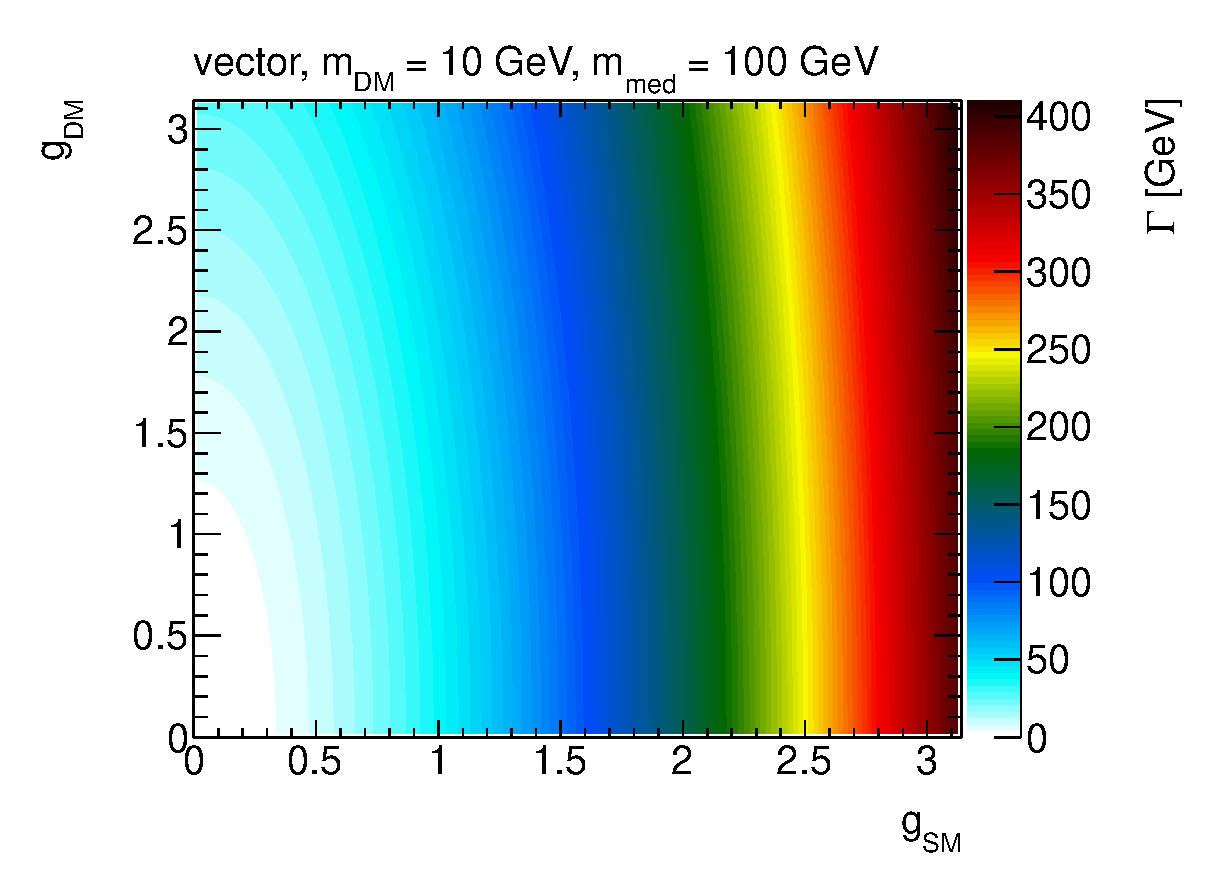
\includegraphics[width=0.49\textwidth]{figures/monojet/constantwidth_V_gg100.eps}
	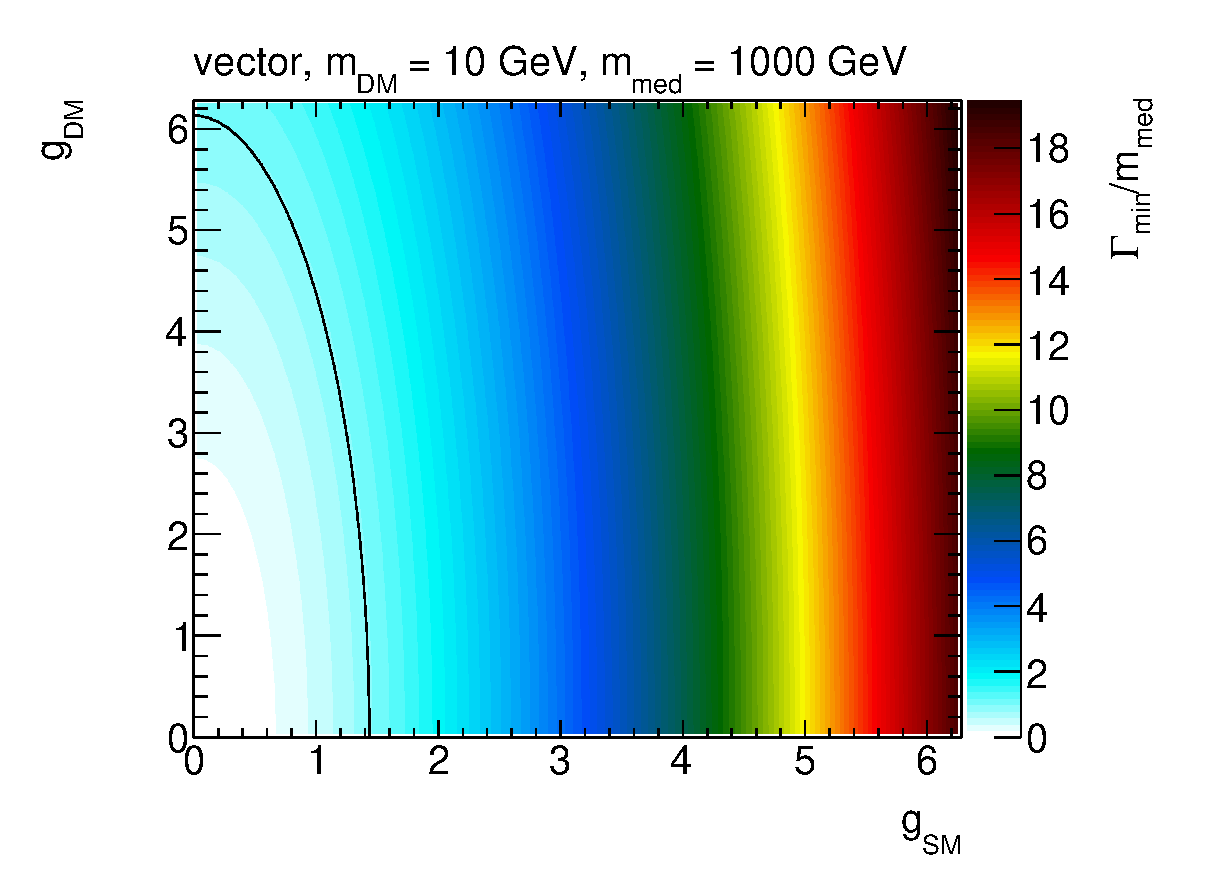
\includegraphics[width=0.49\textwidth]{figures/monojet/constantwidth_V_gg1000.eps}\\
	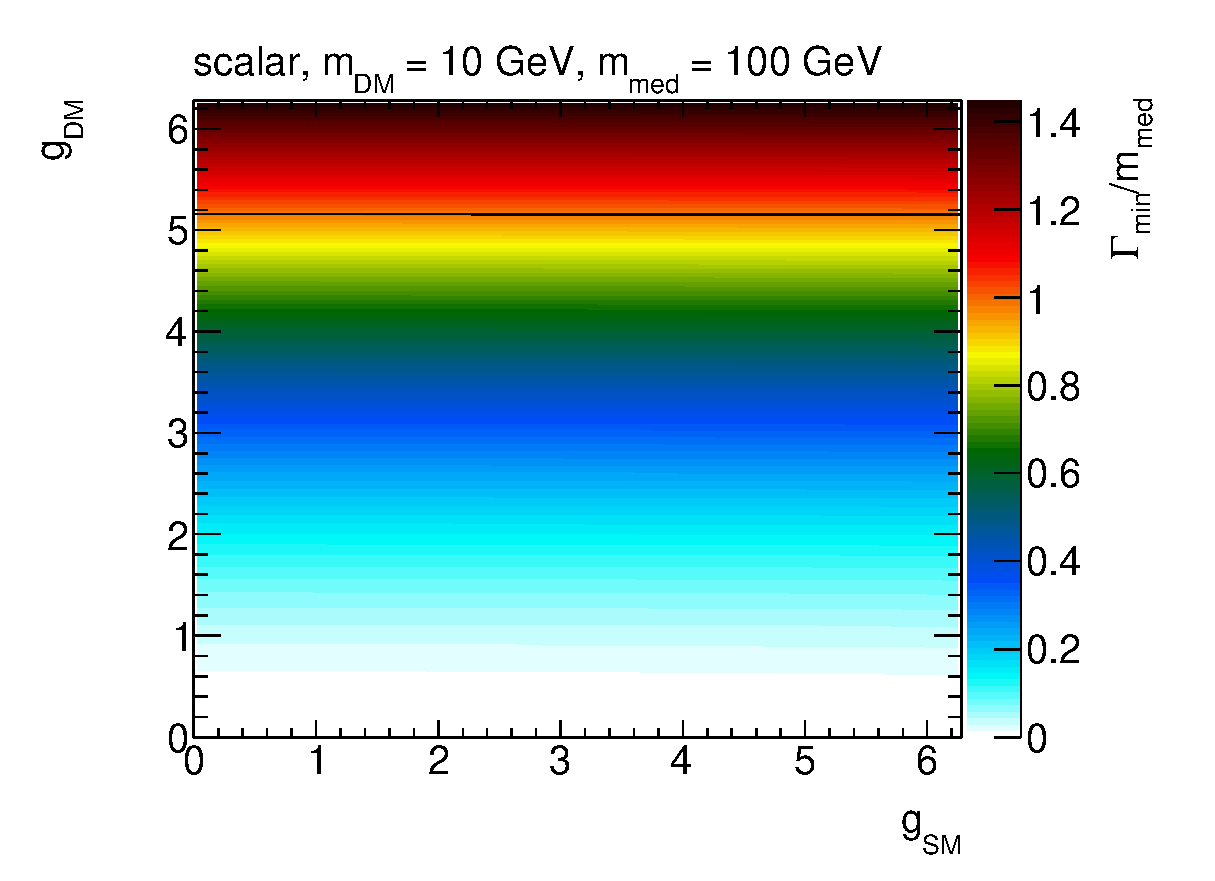
\includegraphics[width=0.49\textwidth]{figures/monojet/constantwidth_S_gg100.eps}
	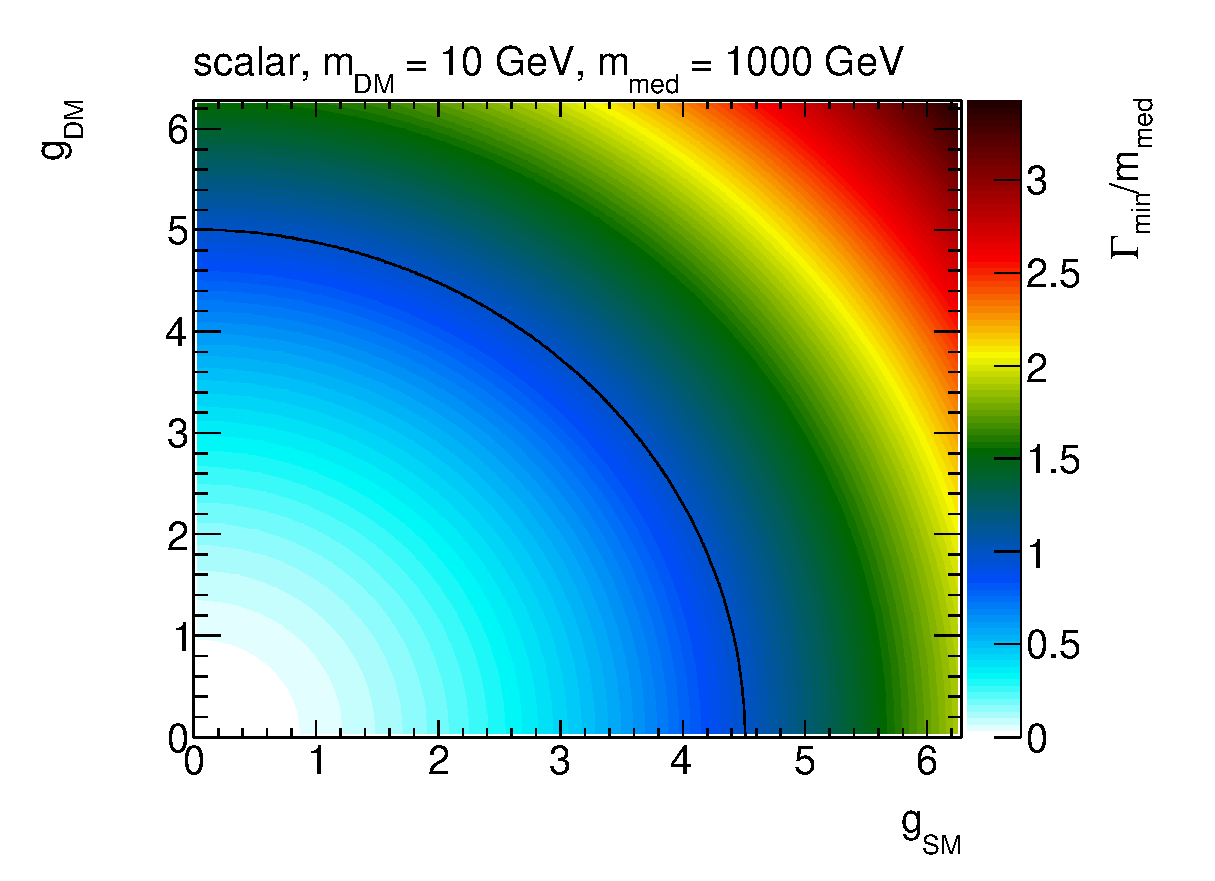
\includegraphics[width=0.49\textwidth]{figures/monojet/constantwidth_S_gg1000.eps}
	\caption{Minimal width over the mediator mass for vector (top) and scalar (bottom) mediators as a function of the individual couplings $\gq$ and $\gDM$, assuming $\mMed=100$~\gev (left) and $\mMed=1$~\tev (right). $\mDM=10$~\gev is considered in all cases.
%		The limiting case $\Gamma_{\rm{min}}=\mMed$ is indicated by the black line.
		Only the cases with $\Gamma_{\rm{min}}<\mMed$ are shown.}
	\label{fig:monojet_width}
\end{figure*}

%\begin{figure}
%	\centering
%	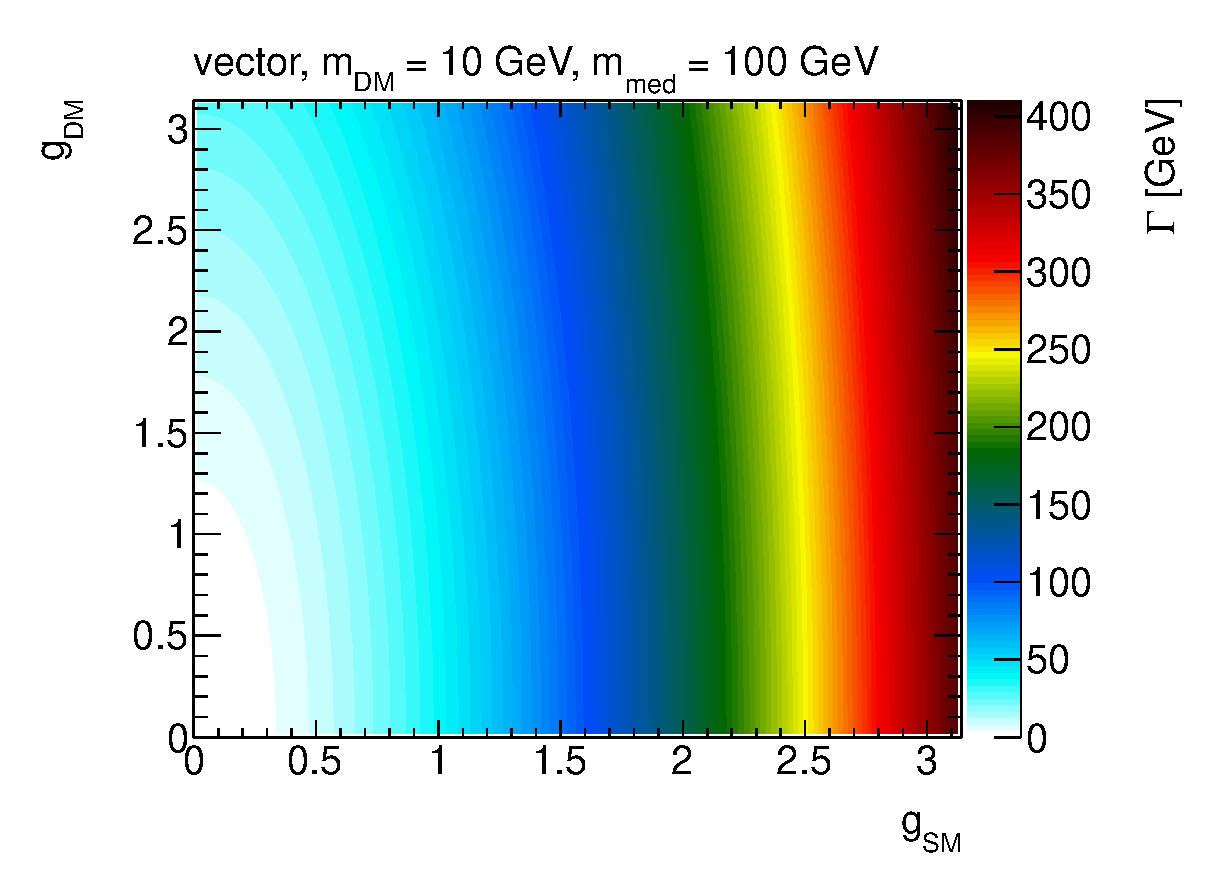
\includegraphics[width=0.95\textwidth]{figures/monojet/constantwidth_V_gg100.eps}
%	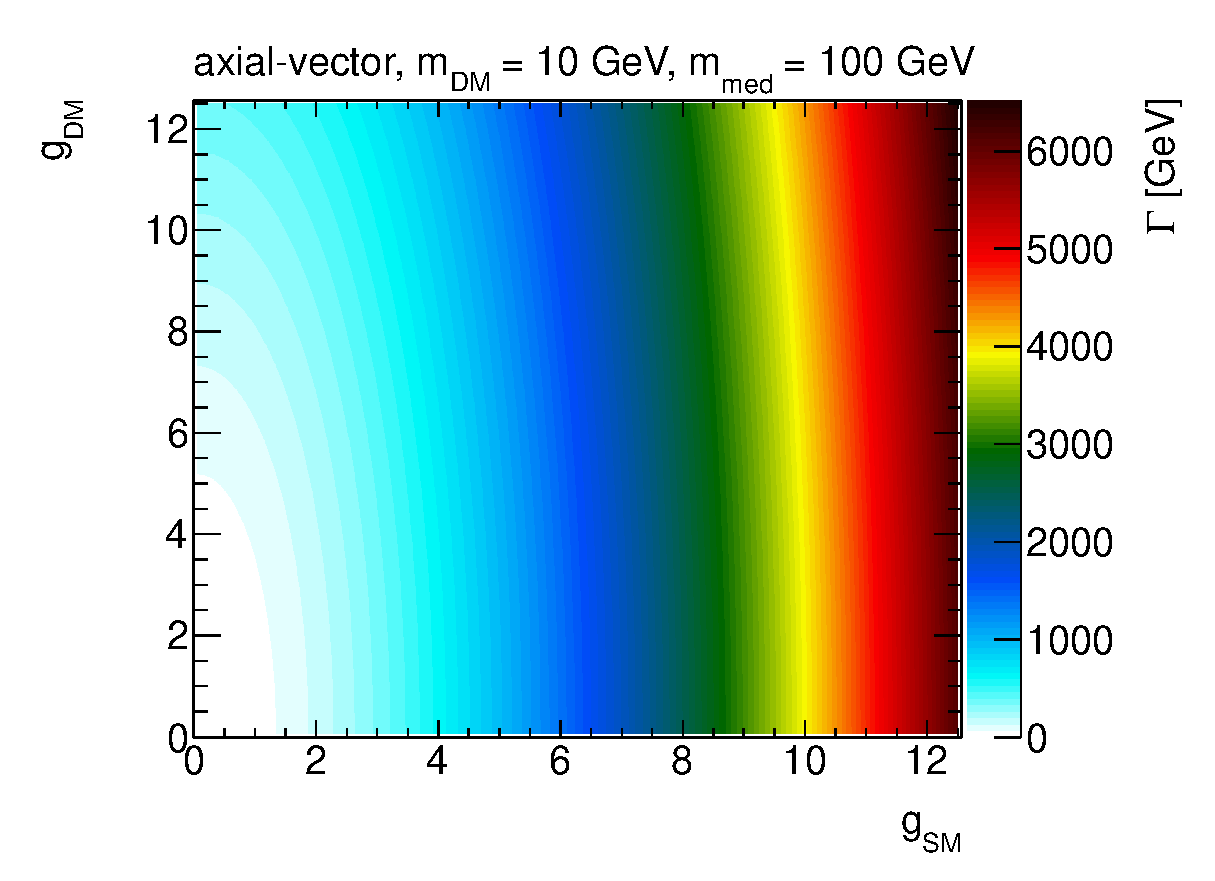
\includegraphics[width=0.95\textwidth]{figures/monojet/constantwidth_A_gg100.eps}\\
%	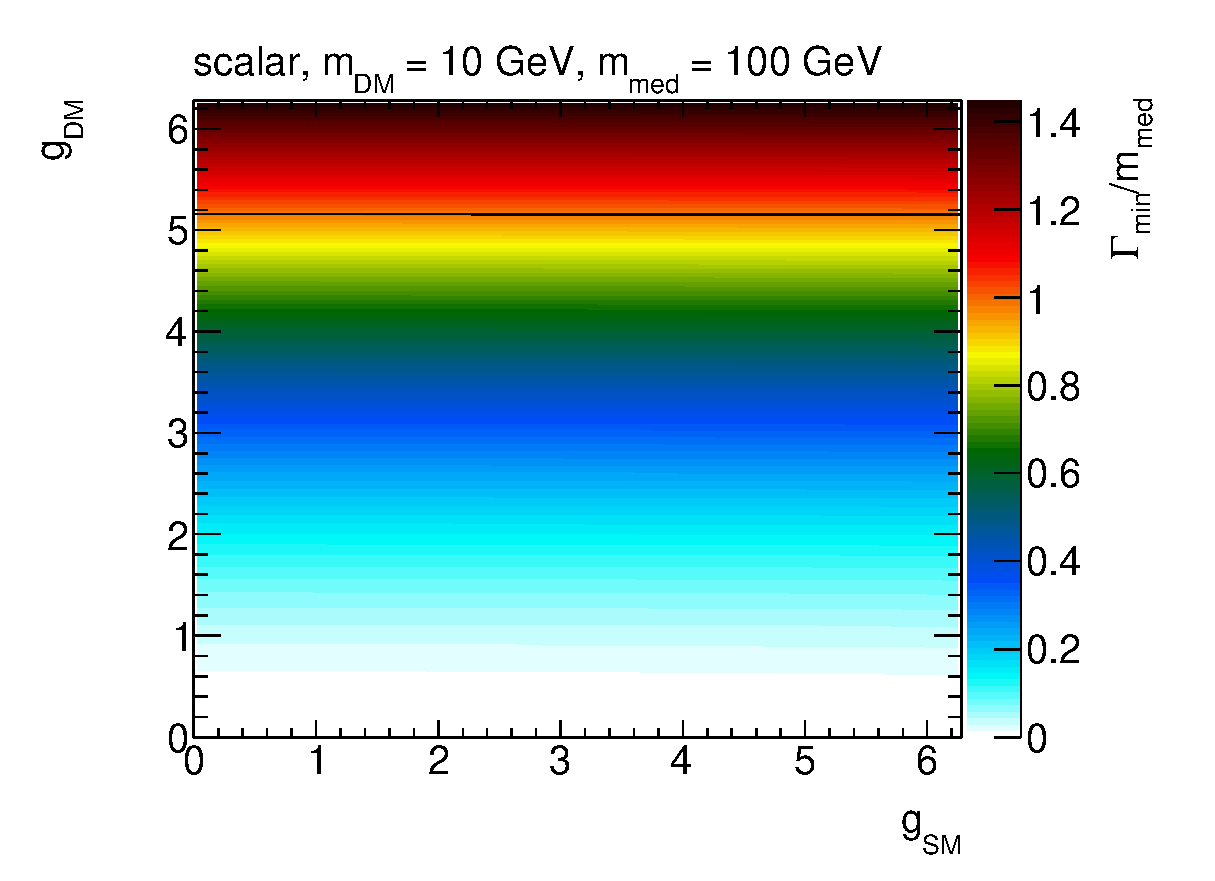
\includegraphics[width=0.95\textwidth]{figures/monojet/constantwidth_S_gg100.eps}
%	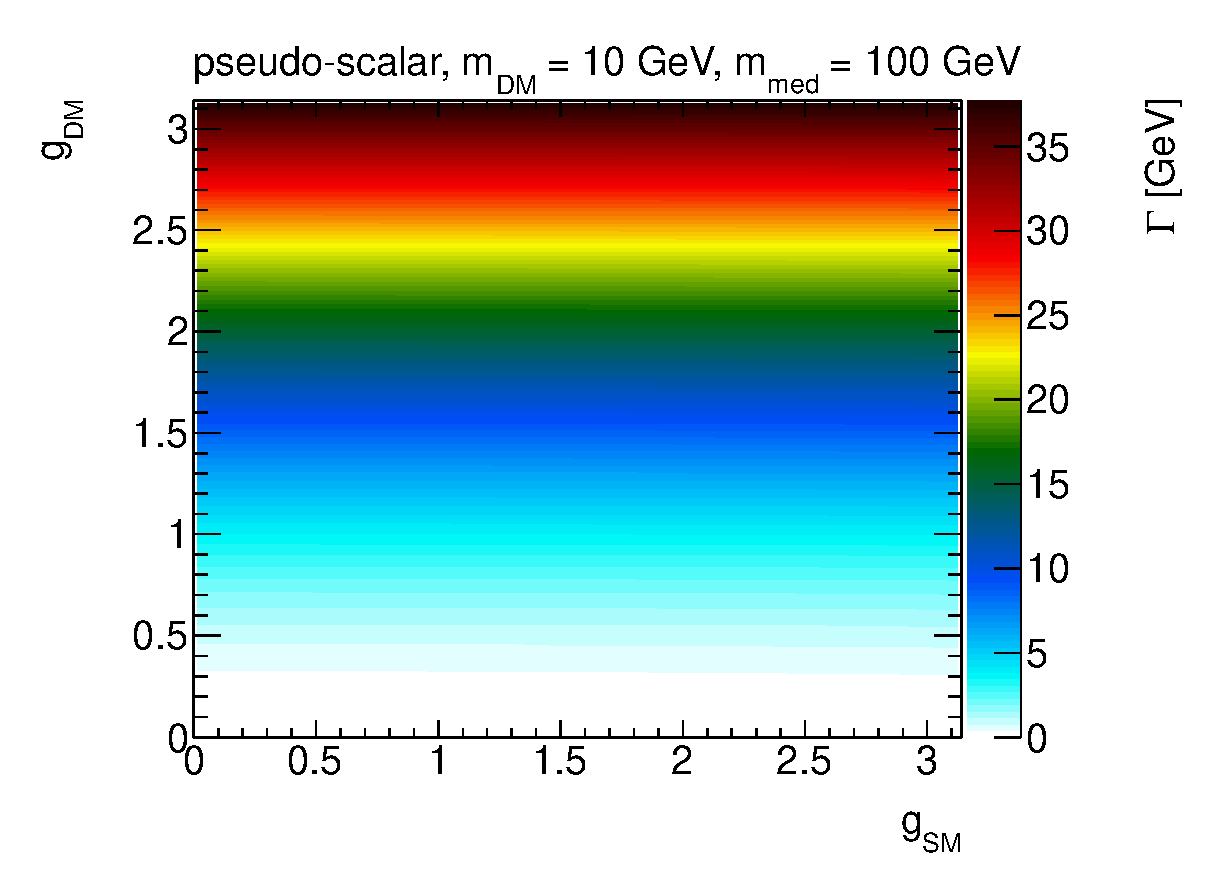
\includegraphics[width=0.95\textwidth]{figures/monojet/constantwidth_P_gg100.eps}
%	\caption{Minimal width over the mediator mass for vector, axial-vector, scalar and pseudo-scalar mediators as a function of the individual couplings $\gq$ and $\gDM$, assuming $\mMed=100$~\gev and $\mDM=10$~\gev.
%		The limiting case $\Gamma_{\rm{min}}=\mMed$ is indicated by the black line.} 
%	\label{fig:monojet_width100}
%\end{figure}
%
%\begin{figure}
%	\centering
%	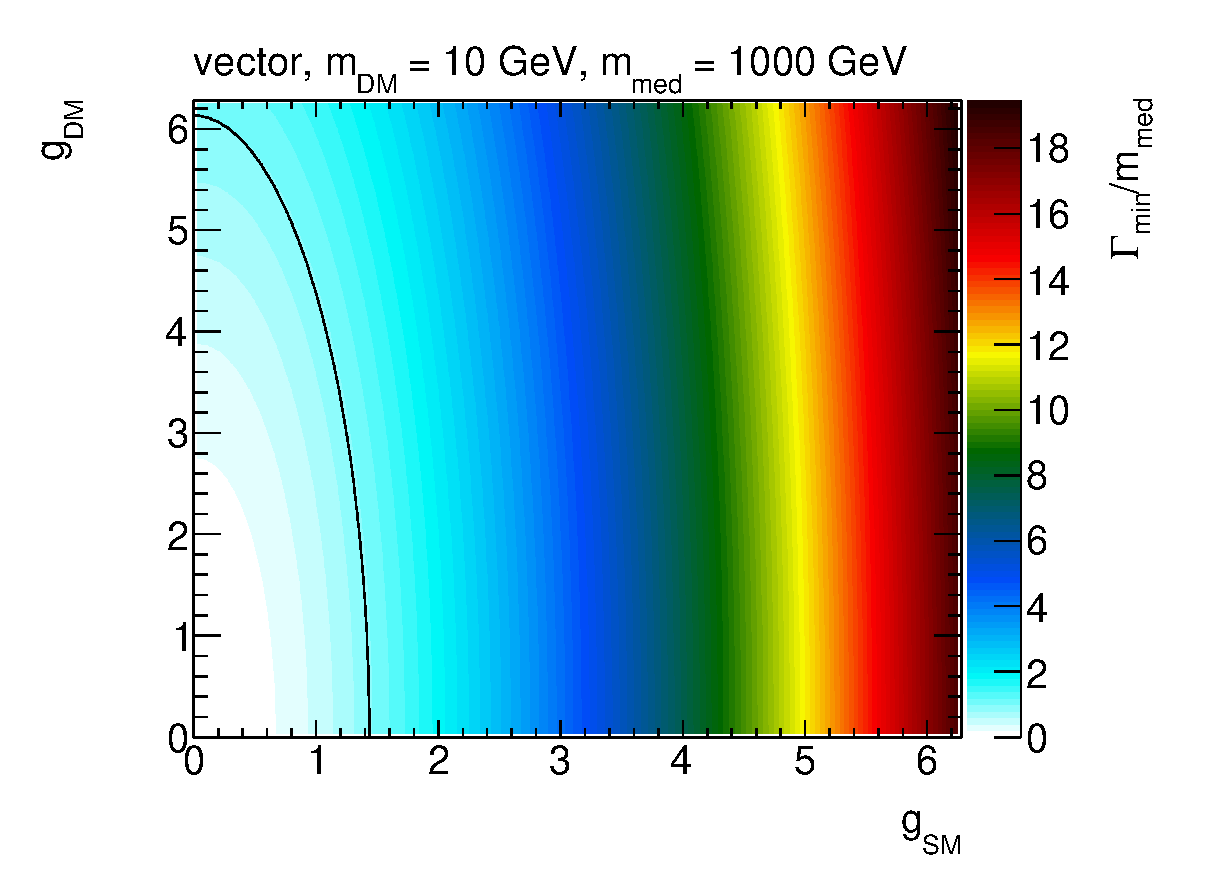
\includegraphics[width=0.95\textwidth]{figures/monojet/constantwidth_V_gg1000.eps}
%	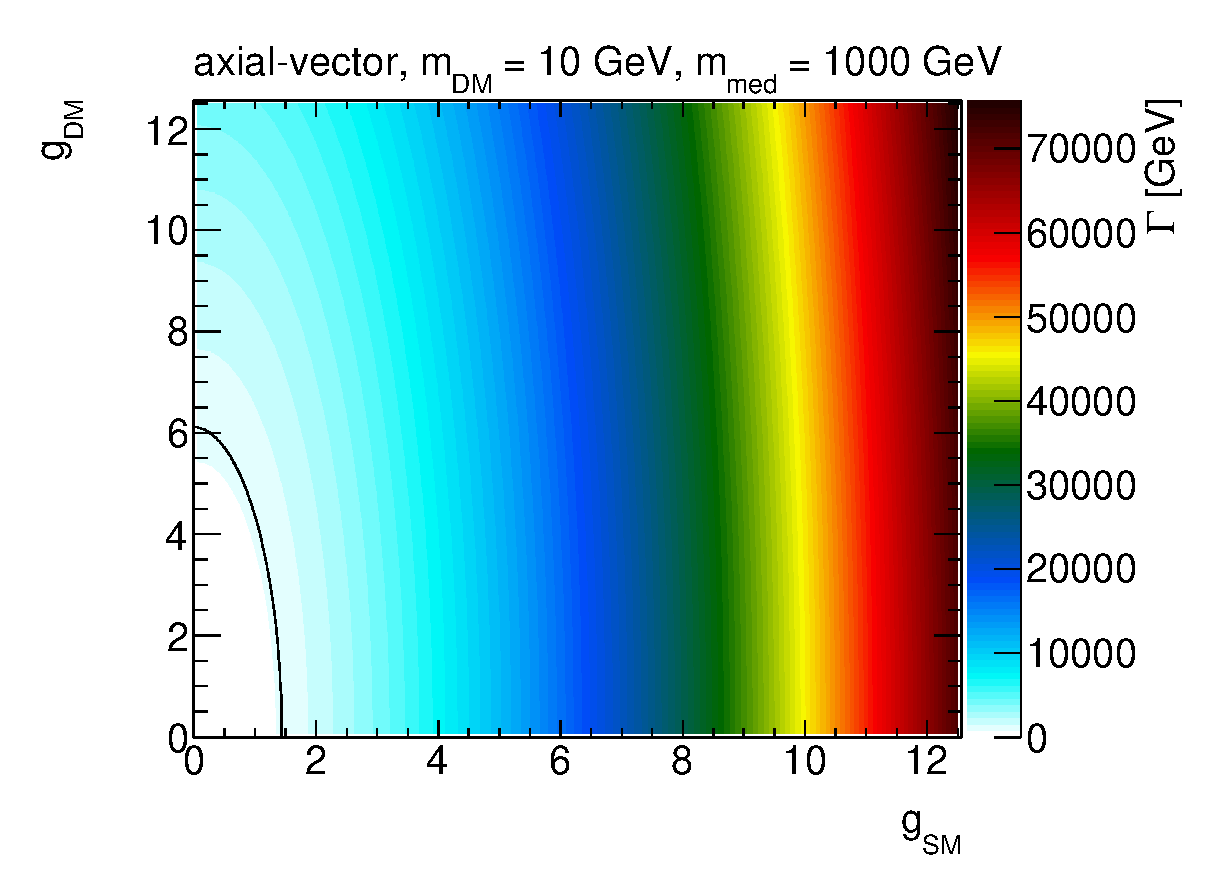
\includegraphics[width=0.95\textwidth]{figures/monojet/constantwidth_A_gg1000.eps}\\
%	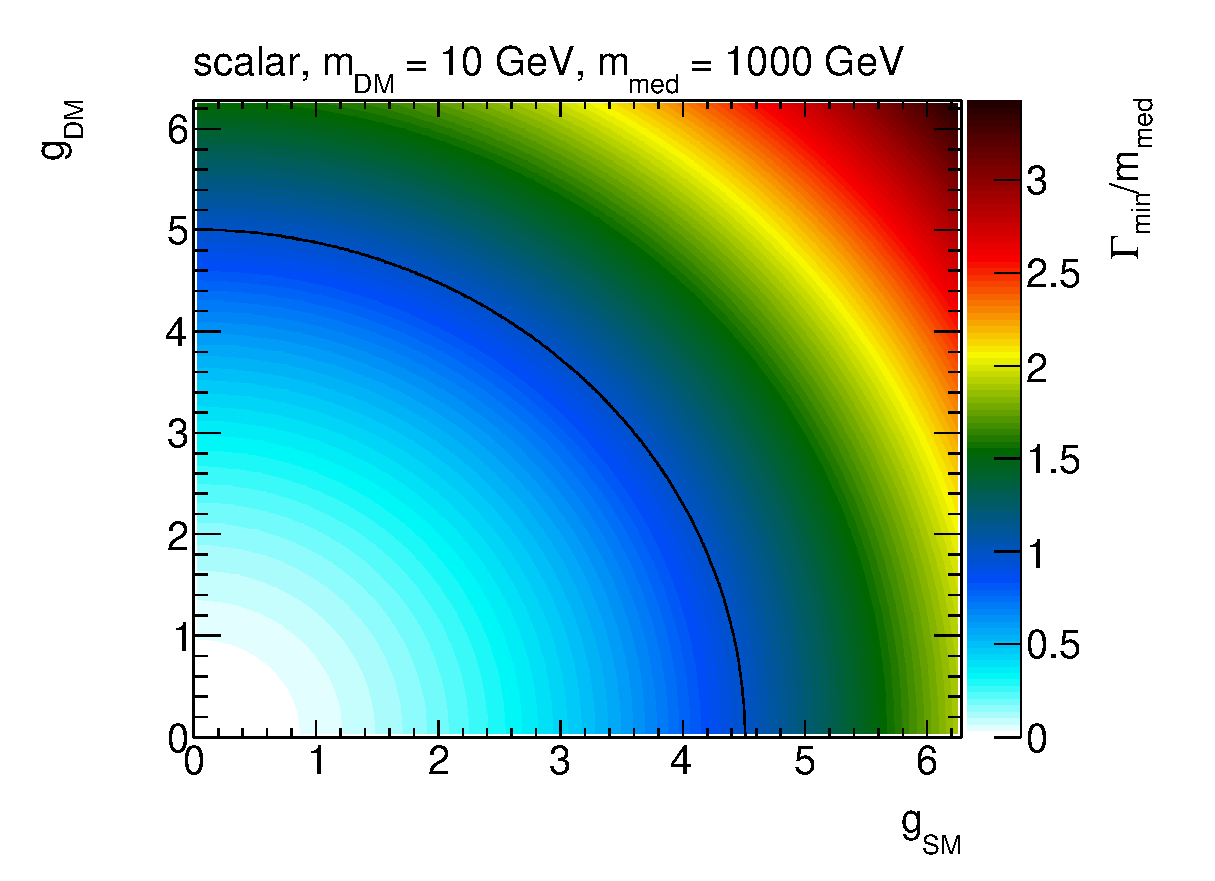
\includegraphics[width=0.95\textwidth]{figures/monojet/constantwidth_S_gg1000.eps}
%	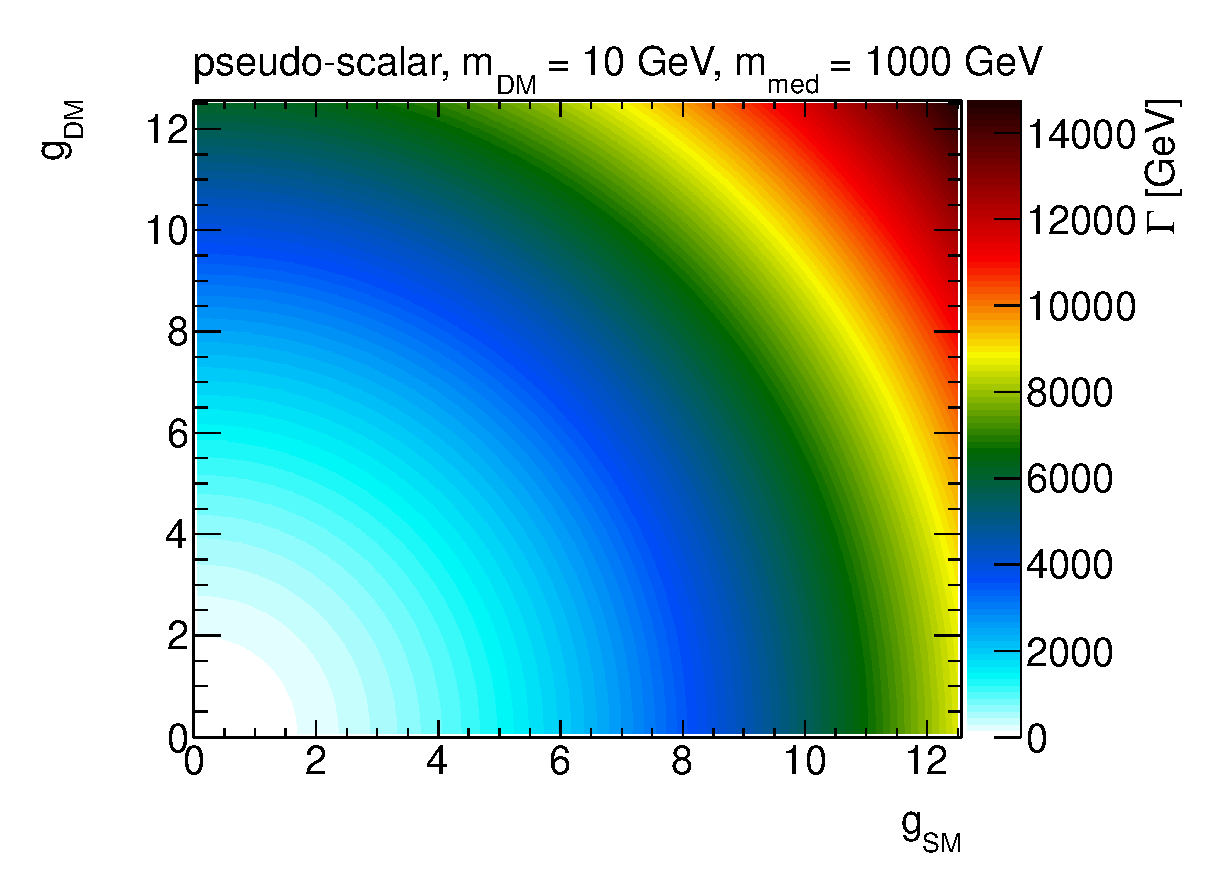
\includegraphics[width=0.95\textwidth]{figures/monojet/constantwidth_P_gg1000.eps}
%	\caption{Minimal width over the mediator mass for vector, axial-vector, scalar and pseudo-scalar mediators as a function of the individual couplings $\gq$ and $\gDM$, assuming $\mMed=1$~\tev and $\mDM=10$~\gev.
%		The limiting case $\Gamma_{\rm{min}}=\mMed$ is indicated by the black line.} 
%	\label{fig:monojet_width1000}
%\end{figure}

%in the plots (gDM = 6, gSM = 1.5 for $V$ and gSM = gDM = 5 for $S$)}


The performance of the cross section scaling is demonstrated in Fig.\,\ref{fig:monojet_scaling} %where two mass points $\mMed=100$~\gev and 1~\tev are chosen with $\mDM=10$~\gev
where two mass points $\mMed=100$~\gev and 1~\tev with $\mDM=10$~\gev are chosen
and rescaled from the starting point $\gq=\gDM=1$ according to Eq.\,\ref{eq:monojet_scaling} to populate the whole $\gq$--$\gDM$ plane. This means the width is not kept constant in this test and this is done in purpose in order to point out deviations from the scaling when the width is altered. For each mass point, the rescaled cross section is compared to the generator cross section and the ratio of the two is plotted.
For the given choice of the mass points, the scaling seems to work approximately within the precision of $\sim20\%$ in the region where $\Gamma_{\rm{min}}<\mMed$.
%For the given choice of the mass points, the scaling seems to work approximately with the precision of $\sim5\%$ for $\Gamma_{\rm{min}}/\mMed<0.1$ and $\sim20\%$ in the region beyond until $\Gamma_{\rm{min}}=\mMed$.
Constant colors indicate the lines along which the cross section scaling works precisely and there is a remarkable resemblance of the patterns shown in the plots of the mediator width. To prove the scaling along the lines of constant width works, one such line is chosen in Fig.\,\ref{fig:monojet_scaling_constwidth} for a scalar mediator, defined by $\mMed=300$~\gev, $\mDM=100$~\gev, $\gq=\gDM=1$, and the rescaled and generated cross sections are found to agree within 3\%.


\begin{figure}
	\centering
	%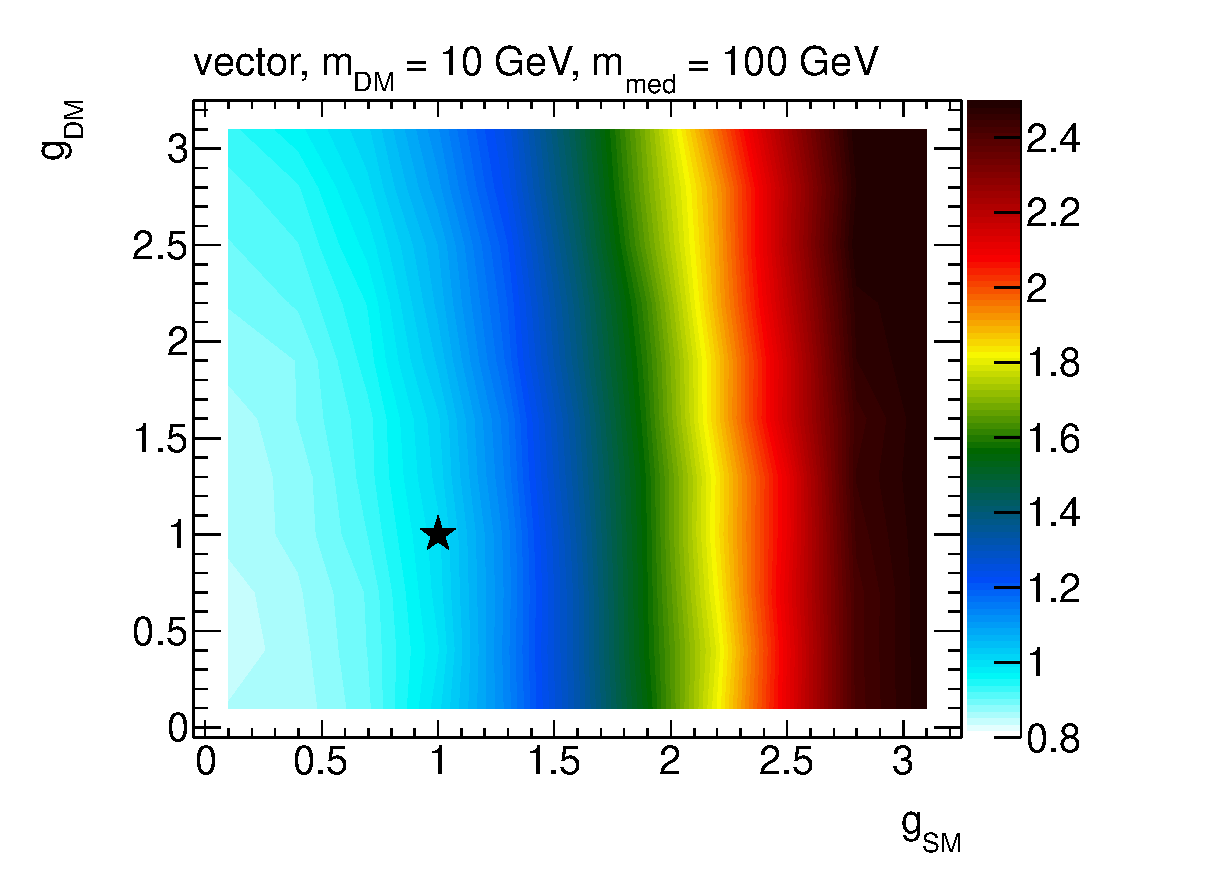
\includegraphics[width=0.95\textwidth]{figures/monojet/scaling_V_10_100.eps}
	%\includegraphics[width=0.95\textwidth]{figures/monojet/scaling_V_10_1000.eps}\\
	\includegraphics[width=0.95\textwidth]{figures/monojet/scaling_S_10_100.eps}
	\includegraphics[width=0.95\textwidth]{figures/monojet/scaling_S_10_1000.eps}\\
	\caption{Ratio of the rescaled and generated cross sections in the $\gq$--$\gDM$ plane. The point at $\gq=\gDM=1$, taken as a reference for the rescaling, is denoted by a star symbol.
		Scalar model with $\mMed=100$~\gev (left) and 1~\tev (right) is plotted for $\mDM=10$~\gev.
		The limiting case $\Gamma_{\rm{min}}=\mMed$ is indicated by a black line and no results are shown beyond.}
	%Vector (scalar) mediator is shown at the top (bottom), the left (right) column corresponds to $\mMed=100$~\gev ($\mMed=1$~\tev). Dark Matter mass of 10~\gev is considered.}
	\label{fig:monojet_scaling}
\end{figure}

%The plots are produced with M_S = 300~\gev, m_chi = 100~\gev, \gSM = \gDM =4
\begin{figure*}
	\centering
	\includegraphics[page=1, trim=310 200 310 200, clip, width=0.49\textwidth]{figures/monojet/rescalingexercise.pdf}
	\includegraphics[page=2, trim=305 195 305 195, clip, width=0.49\textwidth]{figures/monojet/rescalingexercise.pdf}\\
	\includegraphics[page=3, trim=300 190 300 190, clip, width=0.49\textwidth]{figures/monojet/rescalingexercise.pdf}
	\caption{Scaling along the lines of constant width. The line of constant width for $\mMed=300$~\gev and $\mDM=100$~\gev, intercepting $\gq=\gDM=4$ is shown on left. The generated and rescaled cross sections are compared in the middle, the corresponding ratio is shown on right.}
	\label{fig:monojet_scaling_constwidth}
\end{figure*}


\subsection{Proposed parameter grid for cross-section scaling}

We propose to deliver collider results in the $\gq$--$\gDM$ plane using the following prescription, to ease reinterpretation through cross-section scaling:
\begin{itemize}
	\item Since the shapes of kinematic quantities do not change for different couplings, use the acceptance and efficiency for the available $\mDM=50$~\gev, $\mMed=300$~\gev grid point from the $\mMed$--$\mDM$ plane for the scalar and pseudo-scalar mediator. In case of the vector and axial-vector mediator, use the grid point $\mDM=150$~\gev, $\mMed=1$~\tev.
	\item Generate additional samples in order to get generator cross sections only. For scalar and pseudo-scalar mediator, choose $\mDM=50$~\gev, $\mMed=300$~\gev with the following values for $\gq=\gDM$: 0.1, 1, 2, 3. For vector and axial vector mediator, choose $\mDM=150$~\gev, $\mMed=1$~\tev with the following values for $\gq=\gDM$: 0.1, 0.25, 0.5, 0.75, 1, 1.25, 1.5. The upper values are defined by the minimal width reaching the mediator mass. \Todo{Waiting for scalar mediator calculation of perturbativity limit from J. Alcaraz.).}
	\item Rescale the generator cross sections for on-shell resonance production along the lines of constant width in order to populate the whole $\gq$--$\gDM$ plane in the region $\Gamma_{\rm{min}}<\mMed$.
The scaling follows from Eq.\,\ref{eq:monojet_scaling} which for the constant width implies:
\begin{equation}
\sigma' = \sigma \times \frac{\gq'^2\gDM'^2}{\gq^2\gDM^2} \;.
\end{equation}
\end{itemize}

%choose mDM=50, mMed=300, gSM=0.1, gDM={0.1, 1, 2, 3, 4, 5, 6} for S (mMed=GammaMin is reached around 5)
%choose mDM=50, mMed=300, gDM=0.1, gSM={0.1, 0.4, 0.7, 1, 1.3, 1.6, 1.9} for V (mMed=GammaMin is reached around 1.6)
%choose mDM=50, mMed=1000, gDM=0.1, gSM={0.1, 0.4, 0.7, 1, 1.3, 1.6, 1.9} for V (mMed=GammaMin is reached around 1.5)

%choose mDM=50, mMed=300, gSM=gDM={0.1, 1, 2, 3, 4, 5, 6} for S (mMed=GammaMin is reached around 5)
%choose mDM=50, mMed=300, gDM=gSM={0.1, 0.25, 0.5, 0.75, 1, 1.25, 1.5} for V (mMed=GammaMin is reached around 1.5)
%choose mDM=50, mMed=1000, gDM=gSM={0.1, 0.25, 0.5, 0.75, 1, 1.25, 1.5} for V (mMed=GammaMin is reached around 1.4)

\subsection{Rescaling to different mediator width}
\label{paragraph:nonminimalwidth}

In general it is also important to consider a larger mediator width than $\Gamma_{\rm{min}}$ in order to accommodate additional interactions of the mediator with the visible and hidden sector particles~\cite{Buckley:2014fba,Harris:2014hga}. If the narrow width approximation applies, the cross section scaling method described above can be used to reinterpret the results presented for the minimal width, since multiplying the width by factor $n$ is equivalent to changing the coupling strength by factor $\sqrt{n}$, i.e.

\begin{equation}
\sigma(\gq,\gDM, n\Gamma_{\rm{min}}(\gq,\gDM)) \propto \frac{\gq^2 \gDM^2}{\Gamma_{\rm{min}}(\sqrt{n}\gq,\sqrt{n}\gDM)} \;.
\end{equation}
The cross section for the sample with couplings $\gq$ and $\gDM$ and modified mediator width $\Gamma = n\Gamma_{\rm{min}}$ can therefore be rescaled from a sample generated with the minimal width corresponding to the couplings scaled by $\sqrt{n}$ as described in the following formula.

\begin{equation}
\sigma(\gq,\gDM, n\Gamma_{\rm{min}}(\gq,\gDM)) = \frac{1}{n^2} \sigma(\sqrt{n}\gq,\sqrt{n}\gDM,\Gamma_{\rm{min}}(\sqrt{n}\gq,\sqrt{n}\gDM))
\end{equation}
The advantage of doing this is in the fact that no event selection and detector response needs to be simulated since the changes in couplings do not have an effect on the shapes of kinematic distributions.

It should be noted again that this procedure is only useful when the narrow width approximation applies. Care must be taken to ensure that is the case. For example, in the vector and axial-vector cases, one quickly breaks this approximation even for small $n$.

\subsection{\texorpdfstring{Additional considerations for $t \bar{t}$ and $b \bar{b}$+\MET signatures}{Additional considerations for ttbar/bbbar+\MET signatures}}

The cross-section scaling considerations shown in Sec.~\ref{sec:monojet_scaling} still apply for the reactions in the scalar and psuedoscalar models with explicit $b$ and $t$ quarks. Here 
we detail the specific studies done for the  $t\bar t$ model. 

Given that the kinematics are similar for all couplings $g \simeq 1$, we recommend to generate only samples with $\gDM = \gq = 1$. It follows from this that these benchmark points should be a good
approximation for non-unity couplings and for $\gDM \neq \gq$, provided
that the sample is rescaled to the appropriate cross section times
branching ratio.

While the simple scaling function
\begin{equation}
\sigma'\times BR' = [\sigma \times BR]
\times \left( {\gq' \over \gq} \right)^2
\times \left( {\gDM'\over \gDM} \right)^2
\times {\Gamma\over\Gamma'}
\end{equation}
is sufficient for a limited range of coupling values (see Fig.~\ref{fig:xsec_scaling} for example), 
this scaling is only approximate (up to 20\%)  and relies on the narrow width approximation, ignoring PDFs effects. 
%We also choose to provide instead a table of cross section times branching ratio values over a large range of couplings to support interpretation of search results (see the Appendix~\ref{app:TTBar_Xsecs}). The table lists couplings from $g=0.1$ to $g=3.5$, where the upper limit is chosen to be close to but lower than the perturbative limit. 

\begin{figure}[!ht]
	\begin{center}
		\includegraphics[width=0.95\textwidth]{figures/ttbar/xVSwom_mphi_400_mchi_1_proc_S.png}
		\vspace{2mm}
		\caption{\label{fig:xsec_scaling} An example comparing a simple cross section scaling versus the computation from the \madgraph generator, for a scalar $t \bar{t}$+\MET model with $m_{\phi}=400\,{\rm GeV}$, $\mdm=1\,{\rm GeV}$ and all couplings set to unity. In this example, the scaling relationship holds for $\Gamma_{\phi}/m_{\phi}$ below $0.2$, beyond which finite width effects become important and the simple scaling breaks down.}
	\end{center}
\end{figure}

%%%%%%

